%%%%%
%%%%%  Naudokite LUALATEX, ne LATEX.
%%%%%
%%%%
\documentclass[]{VUMIFTemplateClass}

\usepackage{indentfirst}
\usepackage{amsmath, amsthm, amssymb, amsfonts}
\usepackage{mathtools}
\usepackage{physics}
\usepackage{graphicx}
\usepackage{verbatim}
\usepackage[hidelinks]{hyperref}
\usepackage{color,algorithm,algorithmic}
\usepackage[nottoc]{tocbibind}
\usepackage{tocloft}

\usepackage{tikz}
\usetikzlibrary{positioning, arrows.meta, fit, backgrounds}

\usepackage{titlesec}
\newcommand{\sectionbreak}{\clearpage}

\makeatletter
\renewcommand{\fnum@algorithm}{\thealgorithm}
\makeatother
\renewcommand\thealgorithm{\arabic{algorithm} algoritmas}

\usepackage{biblatex}
\bibliography{bibliografija}
%% norint pakeisti bibliografijos šaltinių numeravimą (skaitiniu arba raidiniu), pakeitimus atlikti VUMIFTemplateClass.cls 150 eilutėje

% Author's MACROS
\newcommand{\EE}{\mathbb{E}\,} % Mean
\newcommand{\ee}{{\mathrm e}}  % nice exponent
\newcommand{\RR}{\mathbb{R}}


\studijuprograma{Programų sistemų}
\darbotipas{Bakalauro baigiamasis darbas}
\darbopavadinimas{TurtleBot Burger robotui skirtų aplinkos išžvalgymo algoritmų palyginimas realiose sąlygose}
\darbopavadinimasantras{Comparative Analysis of Environment Exploration Algorithms for the TurtleBot Burger Robot in Real-World Conditions}
\autorius{Gvidas Bačianskas}

\vadovas{prof. dr. Virginijus Marcinkevičius}
\recenzentas{doc. dr. Valentas Gružauskas}

\begin{document}
\selectlanguage{lithuanian}

\onehalfspacing
\begin{titlepage}
\vskip 20pt
\makeatletter

\centerline{\large VILNIAUS UNIVERSITETAS}
\vskip 10pt
\centerline{\large MATEMATIKOS IR INFORMATIKOS FAKULTETAS}
\vskip 10pt
\centerline{\large \MakeUppercase{\@studijuprograma \space studijų programa}}

\vskip 80pt
\centerline{\Large \@darbotipas}
\vskip 20pt
\begin{center}
    {\LARGE \@darbopavadinimas}
\end{center}
\begin{center}
    {\Large \@darbopavadinimasantras}
\end{center}
\vskip 80pt

\hfill
\begin{tabular}{@{}l@{\hspace{1.2cm}}l@{}}
        {Atliko:} & {\@autorius}\\[20pt]
        {Darbo vadovas:} & {\@vadovas}\\[20pt]
        {Darbo recenzentas:} & {\@recenzentas}\\[20pt]
\end{tabular}


\vskip 110pt

\centerline{\large Vilnius – 2026}

\makeatother

\newpage
\end{titlepage}
%\newgeometry{top=2cm,bottom=2cm,right=2cm,left=3cm}
\setcounter{page}{2}


\singlespacing

%Turinys
\tableofcontents
\onehalfspacing

\sectionnonumtoc{Santrauka}{SANTRAUKA}

Autonominiams mobiliesiems robotams, veikiantiems nežinomose vidaus patalpose, nepakanka tik sudaryti aplinkos žemėlapį ir planuoti kelią iki duoto tikslo,
nes robotui taip pat reikia nuspręsti, kurią dar neištirtos aplinkos dalį tirti toliau. Šiame darbe nagrinėjama aplinkos išžvalgymo algoritmų palyginimo
problema: skirtingais sprendimų priėmimo principais pagrįsti metodai gali nevienodai veikti skirtingos geometrijos realiose patalpose. Darbe vienodu
programiniu pagrindu palyginami penki skirtingoms išžvalgymo strategijų grupėms priklausantys algoritmai. Eksperimentai atlikti trijose realiose vidaus
aplinkose: kambaryje su objektais, patalpose su siauru praėjimu tarp jų bei ilgame koridoriuje su nišomis ir kliūtimis. Algoritmai vertinti pagal
išžvalgymo laiką, žemėlapio padengimą, nuvažiuotą kelią ir navigacijos tikslų vykdymo rezultatus. Gauti rezultatai parodė, kad visi nagrinėti algoritmai
gebėjo išžvalgyti realias vidaus patalpas, tačiau jų veikimas priklausė nuo aplinkos geometrijos. Paprastesnėje patalpoje algoritmų rezultatai buvo panašūs, o
siauro praėjimo ir ilgo koridoriaus aplinkose skirtumai išryškėjo labiau. Artimiausios ribos ir informacijos prieaugio metodai daugelyje bandymų pasižymėjo
geru veikimo laiko, nuvažiuoto kelio ir žemėlapio padengimo santykiu. RRT ir Voronoi metodai kai kuriose aplinkose taip pat pasiekė aukštą padengimą, tačiau
jų veikimas buvo mažiau stabilus.

\textbf{Raktiniai žodžiai:} aplinkos išžvalgymas, mobilieji robotai, TurtleBot Burger, ROS~2, Nav2, SLAM, BFS, artimiausia riba, RRT, informacijos prieaugis, Voronoi diagramos.

\sectionnonumtoc{Summary}{SUMMARY}

For autonomous mobile robots operating in unknown indoor environments, it is not sufficient to build a map and plan a path to a given goal, because the robot
also has to decide which unexplored part of the environment should be investigated next. This thesis addresses the comparison of environment exploration
algorithms: methods based on different decision-making principles may perform differently in real indoor environments with different geometries. Five
algorithms belonging to different groups of exploration strategies are compared using a common software basis. The experiments were carried out in three real
indoor environments: a room with objects, a multiple room layout with a narrow passage between the rooms, and a long corridor with alcoves and obstacles. The
algorithms were evaluated using exploration time, map coverage, traveled path length, and navigation goal execution results. The results showed that all
analyzed algorithms were able to explore real indoor environments, but their performance depended on the geometry of the environment. In the simpler room, the
results of the algorithms were similar, while environments with narrow passages and a long corridor revealed clearer differences between the exploration
strategies. The nearest frontier and information gain methods showed a good balance between exploration time, traveled path length, and map coverage in most
experiments. The RRT and Voronoi-based methods also achieved high coverage in some environments, but their performance was less stable.

\textbf{Keywords:} environment exploration, mobile robots, TurtleBot Burger, ROS~2, Nav2, SLAM, BFS, nearest frontier, RRT, information gain, Voronoi diagrams.

\sectionnonumtoc{Įvadas}{ĮVADAS}

Autonominiai mobilieji robotai vis plačiau taikomi vidaus patalpų aplinkose, kuriose reikia savarankiškai judėti, sudaryti aplinkos žemėlapį ir atlikti
užduotis be nuolatinės žmogaus priežiūros. Tokios sistemos itin paplitusios sandėliuose, kosmoso misijose, paieškos ir
gelbėjimo užduotyse. Naujesnėje literatūroje pabrėžiama, kad Robot Operating System 2 (ROS 2) ekosistema ir Navigation2 (Nav2) navigacijos sistema tapo svarbia šiuolaikinių mobiliųjų robotų
programinės įrangos dalimi, nes leidžia kurti modulinę navigacijos, lokalizacijos, planavimo ir valdymo architektūrą~\cite{macenski2022ros2,Nav2-Navigation}. Tačiau net ir turint išvystytą
navigacijos infrastruktūrą, nežinomos aplinkos išžvalgymas išlieka atskira problema: robotas turi nuspręsti, į kurią dar neištirtos aplinkos vietą siųsti kitą
navigacijos tikslą, kad žemėlapis būtų plečiamas efektyviai ir patikimai.

Šiame darbe aplinkos išžvalgymo algoritmai suprantami kaip sprendimų priėmimo metodai, kurie pagal esamą užimtumo tinklą, roboto padėtį ir nežinomos
aplinkos ribas parenka kitą navigacijos tikslą arba tarpinių tikslų seką. Kai yra gaunamas tikslas, žemo lygio kelio planavimą ir judėjimo iki jo
vykdymą atlieka Nav2 sistema. Todėl šiame darbe lyginamas ne žemo lygio kelio planavimas, o aukštesnio lygio išžvalgymo
sprendimas, nuo kurio priklauso, kokias aplinkos sritis robotas bandys pasiekti ir kokia tvarka jos bus tiriamos.

Aplinkos išžvalgymo tyrimai išlieka aktualūs, nes realiose patalpose roboto veikimas priklauso ne tik nuo algoritmo teorinių savybių, bet ir nuo jutiklių,
lokalizacijos, žemėlapio sudarymo bei navigacijos sistemos sąveikos. Išžvalgymo algoritmų literatūroje pabrėžiama, kad robotas turi ne tik sudaryti žemėlapį,
bet ir parinkti tokius tikslus, kurie leistų plėsti žinomą aplinkos dalį įvertinant judėjimo kainą ir pasiekiamumą~\cite{yamauchi1997frontier,keidar2014frontier,pimentel2016infogain}.
Be to, realios sąlygos dažnai skiriasi nuo simuliacijos: jutiklių matavimai gali būti
triukšmingi, odometrijos ir lokalizacijos paklaidos gali kauptis, o sudaromas žemėlapis gali būti netikslus dėl kliūčių, atspindinčių paviršių, siaurų
praėjimų ar aplinkos geometrijos~\cite{SLAM-toolbox,xu2022explorebench}. Dėl to algoritmas, kuris simuliacijoje parenka teoriškai tinkamus tikslus, realiame robote gali generuoti sunkiai
pasiekiamus taškus, sukelti navigacijos nesėkmes arba neefektyviai kartoti judėjimą tose pačiose aplinkos dalyse.

\textbf{Tyrimo problema} formuluojama taip: skirtingais išžvalgymo sprendimų principais pagrįsti algoritmai gali nevienodai veikti skirtingos geometrijos vidaus
patalpose ir realaus TurtleBot Burger roboto apribojimų sąlygomis. Todėl nėra aišku, kurie metodai yra tinkamesni paprastesnėje patalpoje su objektais,
patalpose su siauru praėjimu tarp jų, arba ilgame koridoriuje su nišomis ir kliūtimis, kai visi metodai įgyvendinami vienoje
ROS 2, Nav2 ir vienalaikės lokalizacijos ir žemėlapio sudarymo (angl. \textit{Simultaneous Localization and Mapping}, SLAM) pagrindu veikiančioje sistemoje.

\textbf{Tyrimo objektas} yra aplinkos išžvalgymo algoritmai, taikomi TurtleBot Burger robotui realiomis vidaus patalpų sąlygomis. Darbe sprendžiama vidaus patalpų
išžvalgymo algoritmų palyginimo problema: kaip skirtingi kito navigacijos tikslo parinkimo principai veikia roboto gebėjimą padengti nežinomą aplinką, kiek laiko ir
kelio tam reikia.

\textbf{Darbo tikslas} - palyginti pasirinktus aplinkos išžvalgymo algoritmus, įgyvendintus vienoje ROS 2 ir TurtleBot Burger roboto architektūroje, taikant
palyginamas realių vidaus patalpų eksperimentų sąlygas.


\textbf{Tikslui pasiekti keliami šie uždaviniai:}
\begin{enumerate}
  \item Įvertinti pasirinktų aplinkos išžvalgymo algoritmų grupių teorinius principus ir nustatyti, kodėl jos tinkamos palyginti TurtleBot Burger robotui realiomis
 vidaus patalpų sąlygomis.
 \item Įgyvendinti arba adaptuoti penkis algoritmus vienoje ROS 2 programinėje architektūroje taip, kad jie naudotų tą patį užimtumo tinklą, roboto pozicijos
 gavimą, Nav2 navigacijos tikslų siuntimą ir metrikų registravimą.
 \item Apibrėžti palyginimo kriterijus ir eksperimentų eigą, leidžiančią vertinti algoritmus pagal žemėlapio padengimą, išžvalgymo laiką, nuvažiuotą kelią,
 išsiųstų, pasiektų ir nepavykusių navigacijos tikslų skaičių, o skaičiavimo išteklių naudojimą vertinti kaip papildomą praktinę metriką.
 \item Surinkti palyginamus eksperimentinius duomenis trijose realiose vidaus aplinkose: kambaryje su objektais, patalpose su siauru praėjimu tarp jų
 bei ilgame koridoriuje su nišomis ir kliūtimis.
 \item Palyginti algoritmų rezultatus pagal nustatytas metrikas ir nustatyti, kokiomis aplinkos sąlygomis kiekvienas metodas veikia santykinai geriau arba
 prasčiau.
 \item Suformuluoti praktines rekomendacijas, kuris iš nagrinėtų algoritmų tipų yra tinkamesnis skirtingoms vidaus aplinkų geometrijoms, naudojant tuo pačiu pagrindu veikiančią sistemą.
\end{enumerate}

Darbe lyginami penki algoritmai pasirinkti todėl, kad jie atstovauja skirtingiems išžvalgymo tikslo parinkimo principams. \textbf{BFS} (angl. \textit{Breadth-First Search}) tipo metodas
  atstovauja grafų paieška pagrįstą išžvalgymą~\cite{Introduction-to-Algorithms-book}. \textbf{Artimiausios ribos} (angl. \textit{Nearest Frontier}) metodas atstovauja klasikiniam ribų principui, kai pasirenkama artimiausia
žinomos laisvos erdvės ir nežinomos srities riba~\cite{yamauchi1997frontier}. \textbf{RRT} (angl. \textit{Rapidly-Exploring Random Tree}) metodas atstovauja atsitiktine imtimi ir medžio plėtimu pagrįstą metodų grupę~\cite{umari2017rrt}. \textbf{Informacijos prieaugio} (angl. \textit{Information Gain}) metodas atstovauja
naudingumo funkcija pagrįstą sprendimą, kai vertinama potencialiai gaunama informacija ir judėjimo kaina~\cite{pimentel2016infogain}. \textbf{Voronoi diagramomis pagrįstas} metodas atstovauja geometrijos ir
topologijos principu pagrįstą išžvalgymą, kuriame atsižvelgiama į laisvos erdvės struktūrą ir atstumą nuo kliūčių~\cite{chen2022gvd}. Toks pasirinkimas leidžia palyginti ne tik
atskiras realizacijas, bet ir skirtingas sprendimų priėmimo strategijas.

Šiame darbe pasirinktas palyginimas leidžia praktiškai įvertinti, kaip tie patys penki skirtingų principų algoritmai veikia vienoje tuo pačiu pagrindu sukurtoje sistemoje, realiose vidaus patalpose, atliekant \textbf{pakartotinius bandymus} ir taikant vienodą metrikų rinkinį. Šiame tyrime svarbu
  tai, kad būtent šios realizacijos lyginamos tomis pačiomis fizinio roboto, programinės architektūros ir eksperimentinių aplinkų sąlygomis. Pasirinktos
  aplinkos skiriasi savo struktūra: paprastesnė patalpa leidžia įvertinti algoritmų veikimą mažiau sudėtingoje erdvėje, patalpos su siauru praėjimu išryškina
  tikslo parinkimo ir pasiekiamumo problemas, o ilgas koridorius leidžia įvertinti algoritmų elgseną pailgos geometrijos aplinkoje. Todėl darbe daugiausia
  dėmesio skiriama tam, kaip skirtingi išžvalgymo sprendimų principai prisitaiko prie skirtingų vidaus aplinkų struktūrų.

\section[LITERATŪROS ANALIZĖ]{Literatūros analizė}

Šio skyriaus tikslas - išanalizuoti literatūroje aprašomus autonominių mobiliųjų robotų aplinkos išžvalgymo principus ir įvertinti, kurie metodai yra tinkami
palyginti naudojant \textit{TurtleBot Burger} robotą realiomis vidaus patalpų sąlygomis. Taip pat siekiama įvertinti, kokie literatūroje aprašomi veiksniai
turi įtakos algoritmų veikimui realiame robote, kai aplinkos modelis sudaromas iš lazerinio atstumo jutiklio (angl. \textit{Light Detection and Ranging}, LiDAR) duomenų. Literatūros analize siekiama pagrįsti
šiame darbe pasirinktų algoritmų grupes, palyginimo kriterijus ir eksperimentinių aplinkų pasirinkimą.

\textbf{Analizėje keliami šie klausimai:}
\begin{enumerate}
  \item Kokie autonominio išžvalgymo sprendimų priėmimo principai dažniausiai taikomi mobiliųjų robotų vidaus aplinkų tyrimui?
  \item Kokie yra ribomis, grafais, atsitiktine imtimi, informacijos prieaugiu ir geometrija pagrįstų metodų privalumai bei ribojimai?
  \item Kaip SLAM, užimtumo tinklas ir Nav2 navigacijos sistema susiję su aplinkos išžvalgymo algoritmo veikimu?
  \item Kurie iš nagrinėjamų aplinkos išžvalgymo algoritmų realiomis sąlygomis, naudojant \textit{TurtleBot Burger} robotą ir LiDAR jutiklio
   duomenis, leidžia efektyviausiai ir patikimiausiai išžvalgyti vidaus patalpas?
  \item Kokios eksperimentinės aplinkos ir metrikos leidžia pagrįstai palyginti aplinkos išžvalgymo algoritmus realiomis sąlygomis?
\end{enumerate}

Autonominių mobiliųjų robotų veikimas vidaus patalpose remiasi kelių tarpusavyje susijusių komponentų sąveika: aplinkos suvokimu, lokalizacija, žemėlapio
sudarymu, kelio planavimu, kliūčių vengimu ir aukštesnio lygio sprendimų priėmimu. Vidaus aplinkose robotas dažniausiai negali remtis GPS ar kitomis išorinėmis
globalios padėties nustatymo sistemomis, todėl turi naudoti jutiklius ir programinius algoritmus, leidžiančius vienu metu įvertinti savo padėtį, aptikti
kliūtis ir sudaryti aplinkos modelį.

Šiame skyriuje apžvelgiamos pagrindinės technologijos ir algoritminiai principai, reikalingi aplinkos išžvalgymo algoritmų palyginimui.

\subsection{Autonominių robotų navigacijos technologijos}
Autonominio roboto navigacijos sistema yra sudėtinga ir sudaryta iš kelių tarpusavyje sąveikaujančių technologinių komponentų. Siekiant užtikrinti patikimą ir lankstų roboto veikimą, šios sistemos dažniausiai projektuojamos \textbf{sluoksniuotos architektūros principu}, atskiriant žemo lygio valdymą nuo aukšto lygio sprendimų priėmimo.

„TurtleBot3 Burger" platforma \cite{Turtlebot3-overview, TURTLEBOT3-AS-EDUCATION-PLATFORM} yra tipinis modulinės robotinės sistemos pavyzdys. Toliau šiame poskyryje apžvelgiami pagrindiniai technologiniai komponentai, kurie naudojami roboto navigacijos ir aplinkos išžvalgymo uždaviniams spręsti, bei jų vaidmuo bendroje sistemos struktūroje.

\subsubsection{Mobiliojo roboto valdymo architektūra}

Autonominių robotų navigacijos sistemos dažniausiai projektuojamos atskiriant žemo lygio valdymą nuo aukšto lygio skaičiavimų. Žemajame lygyje naudojamas mikrovaldiklis atsakingas už tiesioginę sąveiką su fiziniais komponentais - variklių valdymą, odometrijos duomenų nuskaitymą ir realaus laiko operacijas. Aukštajame lygyje veikia pagrindinis kompiuteris, kuris vykdo sudėtingesnius algoritmus, tokius kaip SLAM ir aplinkos išžvalgymas.

Šių dviejų lygių sąveika pateikta \ref{fig:high-low-architecture} pav. Aukšto lygio sistemoje sudaromas žemėlapis, parenkamas išžvalgymo tikslas ir planuojamas
roboto judėjimas. Žemo lygio sistema vykdo greičio komandas, valdo variklius ir pagal roboto judėjimą teikia odometrijos duomenis. Jutiklių duomenys naudojami
aplinkos matavimams ir žemėlapio atnaujinimui.

\begin{figure}[H]
\centering
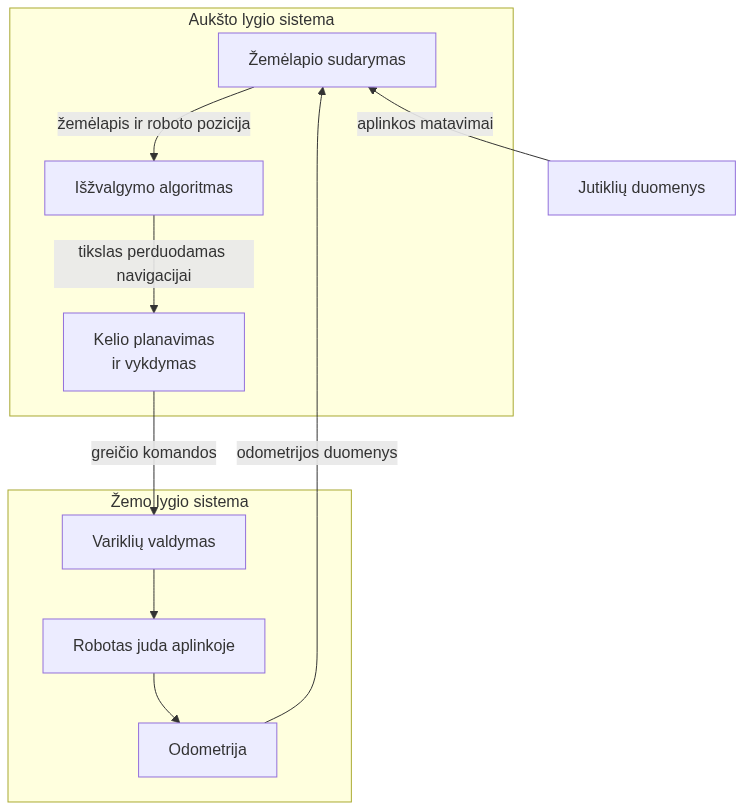
\includegraphics[width=0.7\textwidth]{images/diagramos/hi-lo-arch.png}
\caption{Aukšto ir žemo lygio roboto sistemos sąveika}
\label{fig:high-low-architecture}
\end{figure}

„TurtleBot3" platformoje šią architektūrą realizuoja „OpenCR" mikrovaldiklis \cite{OpenCR-puslapis} ir „Raspberry Pi" mikrokompiuteris \cite{RPi-puslapis}. Mikrovaldiklis veikia kaip tarpinė grandis tarp aukšto lygio skaičiavimo sistemos ir fizinės roboto įrangos, užtikrindamas deterministinį veikimą realiuoju laiku. „Raspberry Pi" kompiuteris suteikia pakankamai procesoriaus galios ir operatyviosios atminties navigacijos algoritmams vykdyti, o taip pat leidžia diegti pilnavertes operacines sistemas ir programinius karkasus, tokius kaip ROS.

Toks architektūrinis sprendimas leidžia efektyviai paskirstyti skaičiavimo apkrovą - žemo lygio valdymo funkcijos vykdomos nepriklausomai nuo pagrindinio kompiuterio apkrovos, taip padidinant visos sistemos patikimumą ir palengvinant programinės įrangos plėtrą.

\subsubsection{ROS 2 karkasas}

Svarbi šiuolaikinės robotikos programinės įrangos dalis yra ROS~2. Literatūroje ROS~2 aprašoma kaip \textbf{modulinė robotikos programinė aplinka}, skirta paskirstytoms robotų sistemoms kurti ir vykdyti~\cite{macenski2022ros2}. Ji remiasi atskirų programinių mazgų sąveika: skirtingi komponentai gali publikuoti ir prenumeruoti pranešimus, naudoti paslaugas, veiksmų sąsajas ir transformacijų medį. Tokia architektūra leidžia atskirti jutiklių duomenų gavimą, roboto būsenos publikavimą, žemėlapio sudarymą, navigaciją ir aukštesnio lygio sprendimų priėmimą į savarankiškus, bet tarpusavyje susietus komponentus.

\textbf{ROS~2 svarba} aplinkos išžvalgymo algoritmų tyrimuose siejama su tuo, kad ši aplinka leidžia algoritmus integruoti į bendrą robotinę sistemą nekeičiant žemo lygio valdymo, jutiklių apdorojimo ar navigacijos komponentų. Todėl skirtingi išžvalgymo metodai gali būti realizuojami kaip atskiri programiniai komponentai, kurie naudoja tą pačią įvesties informaciją ir perduoda rezultatus tomis pačiomis ROS~2 sąsajomis.

\subsubsection{Nav2 navigacijos sistema}

Nav2 sistema literatūroje aprašoma kaip ROS~2 pagrindu veikianti mobiliosios navigacijos infrastruktūra, skirta kelio planavimui, judėjimo valdymui, kliūčių vengimui ir atkūrimo veiksmams~\cite{Nav2-Navigation}. Tyrime pabrėžiama, kad Nav2 architektūra yra modulinė, paremta elgsenos medžiais, atskirais planavimo ir valdymo serveriais bei konfigūruojamais įskiepiais.

Tokia architektūra yra svarbi aplinkos išžvalgymo algoritmų analizei, nes ji leidžia atskirti \textbf{aukšto lygio tikslo parinkimą} nuo kelio planavimo ir judėjimo vykdymo. Išžvalgymo algoritmas gali būti nagrinėjamas kaip komponentas, kuris parenka kitą navigacijos tikslą, o kelio iki šio tikslo planavimas, kliūčių vengimas ir judėjimo vykdymas perduodami bendrai navigacijos infrastruktūrai.

\subsubsection{Jutikliai aplinkos suvokimui}

Aplinkos suvokimas yra viena svarbiausių autonominio mobiliojo roboto funkcijų, nuo kurios tiesiogiai priklauso navigacijos ir aplinkos išžvalgymo algoritmų veikimas. Siekiant sudaryti aplinkos žemėlapį ir aptikti kliūtis, mobiliuosiuose robotuose naudojami įvairūs jutikliai, tokie kaip ultragarsiniai davikliai, kameros ar lazeriniai atstumų matuokliai.

Autonominiuose mobiliuosiuose robotuose aplinkos suvokimui gali būti naudojami skirtingi jutikliai. Kameros suteikia daug vizualinės informacijos, tačiau jų
veikimas priklauso nuo apšvietimo sąlygų ir reikalauja sudėtingesnio vaizdų apdorojimo. Ultragarsiniai ir infraraudonųjų spindulių jutikliai gali būti
naudojami artimoms kliūtims aptikti, bet jų tikslumas ir veikimo nuotolis yra riboti. Inerciniai jutikliai ir ratų enkoderiai padeda įvertinti roboto
judėjimą, tačiau patys nesuteikia pakankamai informacijos nežinomos aplinkos žemėlapiui sudaryti. Dėl šių priežasčių patalpų navigacijos ir išžvalgymo
uždaviniuose dažnai naudojami lazeriniai atstumo jutikliai.

Patalpų navigacijos uždaviniuose dažnai naudojami LiDAR jutikliai, nes jie leidžia tiksliai ir greitai nustatyti atstumą iki aplinkinių objektų. LiDAR jutikliai skleidžia lazerio spindulį ir, matuodami jo atspindžio laiką, apskaičiuoja atstumą iki kliūties, taip sudarydami dvimatį atstumų matavimų rinkinį.

Dėl plataus matymo kampo ir pakankamo atnaujinimo dažnio lazeriniai jutikliai yra tinkami autonominiam patalpų išžvalgymui. Jie suteikia roboto navigacijos sistemai nuoseklius ir struktūrizuotus duomenis, kurie gali būti tiesiogiai naudojami žemėlapių sudarymo ir sprendimų priėmimo algoritmuose. Be to, LiDAR jutiklių duomenys yra mažiau jautrūs apšvietimo sąlygoms nei vaizdo kameros, todėl jie laikomi patikimu sprendimu vidaus aplinkose \cite{LDS-02-puslapis}.

\subsubsection{Judėjimo sistema ir odometrija}

Mobiliųjų robotų judėjimas realizuojamas naudojant elektromechanines pavaras, kurios leidžia robotui keisti padėtį erdvėje ir vykdyti planuotą trajektoriją. Vidaus patalpų navigacijoje dažniausiai naudojami ratais varomi robotai, pasižymintys paprasta mechanine konstrukcija ir pakankamu manevringumu.

Vienas iš plačiai taikomų sprendimų yra diferencinio valdymo schema, kai robotas turi du nepriklausomai valdomus varomuosius ratus. Keičiant ratų sukimosi greitį, robotas gali judėti tiesiai, suktis vietoje arba važiuoti lenkta trajektorija. Dėl savo paprastumo ir efektyvumo ši valdymo schema naudojama tiek edukacinėse, tiek tyrimų platformose. Nors tokia konstrukcija pasižymi paprastumu ir yra plačiai naudojama moksliniuose tyrimuose bei edukacinėse platformose, jos pozicijos nustatymo tikslumas realioje aplinkoje gali mažėti dėl ratų praslydimo, nevienodo paviršiaus bei odometrinių matavimų paklaidų \cite{odometry-drift}.

Svarbus judėjimo sistemos komponentas yra odometrija - roboto nueito kelio apskaičiavimas pagal ratų apsisukimų skaičių. Dauguma mobiliųjų robotų naudoja variklius su integruotais koduotojais (angl. \textit{Encoder}), kurie leidžia matuoti ratų poziciją ir greitį \cite{Dynamixel-motor-puslapis}. Odometrijos duomenys yra būtini navigacijos sistemai, nes suteikia informaciją apie roboto judėjimą tarp jutiklių matavimų. Tačiau dėl ratų praslydimo ir mechaninių paklaidų \textbf{odometrija ilgainiui kaupia klaidas}, todėl ją būtina derinti su kitais lokalizacijos metodais, tokiais kaip SLAM.


\subsection{SLAM ir užimtumo tinklo reprezentacija}

Kad robotas galėtų judėti nežinomoje patalpoje, jam reikia aplinkos modelio. Ši problema literatūroje apibrėžiama kaip \textbf{SLAM} (angl. \textit{Simultaneous
Localization and Mapping}) - vienalaikė lokalizacija ir žemėlapio sudarymas. SLAM yra viena iš pagrindinių mobiliosios robotikos problemų, nes lokalizacija ir
žemėlapio sudarymas tarpusavyje priklauso vienas nuo kito. Netiksli roboto padėtis lemia netikslų žemėlapį, o netikslus žemėlapis apsunkina tolimesnę
lokalizaciją.

Literatūroje pažymima, kad per pastaruosius du dešimtmečius SLAM tapo pagrindiniu autonominių mobiliųjų robotų komponentu, o tyrimų dėmesys vis labiau
krypsta
į ilgalaikį, patikimą veikimą realiose ir dinamiškose aplinkose~\cite{slam-past-present-future}.                                                                                        
SLAM metodai skirstomi į filtravimo ir optimizavimo metodus. Filtravimo metodai, pavyzdžiui, dalelių filtrai, būseną atnaujina nuosekliai, gavus naujus jutiklių
duomenis. Grafų optimizavimo metodai roboto trajektoriją vaizduoja kaip grafą, kurio viršūnės atitinka roboto pozicijas, o briaunos - judėjimo ar jutiklių matavimų apribojimus. Tokiuose metoduose žemėlapio nuoseklumas gerinamas optimizuojant visą pozicijų grafą. Pastaruoju metu grafais pagrįsti SLAM metodai tapo
dominuojančiu           
standartu dėl jų tikslumo ir gebėjimo tvarkyti kilpų uždarymo (angl. \textit{loop closure}) problemą.

Šiame darbe naudojamas \textit{slam\_toolbox} \cite{SLAM-toolbox}, kuris yra ROS aplinkai skirtas grafais pagrįstas SLAM sprendimas. Jis leidžia realiuoju laiku kurti dvimatį
\textbf{užimtumo tinklą}  \cite{Occupancy-grid}, naudojamą tolimesnei navigacijai ir aplinkos išžvalgymui. Užimtumo tinklas yra viena dažniausių aplinkos reprezentacijų mobiliųjų robotų
navigacijoje. Jame aplinka suskaidoma į langelius, kurių būsena gali būti \textbf{laisva, užimta arba nežinoma}. Tokia reprezentacija patogi todėl, kad ji
tiesiogiai leidžia identifikuoti kliūtis, laisvas judėjimo zonas ir dar neištirtas aplinkos dalis.

Užimtumo tinklas taip pat yra pagrindas daugeliui aplinkos išžvalgymo algoritmų. Ribomis pagrįsti metodai naudoja perėjimą tarp laisvų ir nežinomų langelių. BFS
tipo metodai ieško pasiekiamų langelių per žinomą laisvą erdvę. RRT metodai gali plėsti medį per žinomą erdvę iki nežinomų sričių. Informacijos prieaugio
metodai vertina, kiek nežinomų langelių galėtų būti stebima iš kandidatinio tikslo. Voronoi metodai analizuoja laisvos erdvės geometriją ir atstumą iki kliūčių.
Todėl užimtumo tinklas šiame darbe yra bendra duomenų struktūra, leidžianti penkis skirtingus algoritmus įgyvendinti toje pačioje sistemoje.

\subsection{Nežinomos aplinkos išžvalgymo problema}

\textbf{SLAM savaime nenurodo, kur robotas turėtų judėti}, kad aplinka būtų ištirta efektyviai. Jis sudaro ir atnaujina žemėlapį pagal roboto judėjimą, tačiau sprendimas, kurią aplinkos dalį tirti toliau, priklauso aplinkos išžvalgymo algoritmui. Literatūroje ši užduotis apibrėžiama kaip aktyvaus SLAM (angl. \textit{active SLAM}) problema - roboto judėjimo planavimo ir valdymo uždavinys, kurio tikslas yra sudaryti kuo tikslesnį ir išsamesnį nežinomos aplinkos modelį. Tokioje sistemoje
robotas turi pasirinkti būsimus veiksmus, derindamas naujų sričių tyrimą su jau žinomų sričių panaudojimu lokalizacijai ir žemėlapio tikslumui gerinti~\cite{placed2023activeslam}.
                                                                                                                          
Daugelyje praktinių sistemų aplinkos išžvalgymo procesą galima suskaidyti į tris dalis: kandidatinių tikslų identifikavimą, jų įvertinimą ir pasirinkto tikslo
vykdymą. Ši schema tiesiogiai atitinka šiame darbe nagrinėjamą architektūrą: algoritmai analizuoja užimtumo tinklą ir parenka kitą navigacijos tikslą, o      
pasirinkto tikslo vykdymas perduodamas Nav2 sistemai. Taigi lyginami algoritmai skiriasi ne tuo, kaip jie lokaliai valdo roboto ratus ar planuoja trajektoriją
iki tikslo, bet tuo, kokią aplinkos vietą jie laiko tinkamiausia tirti toliau. 

Klasikinė nežinomos aplinkos išžvalgymo problema dažnai formuluojama per ribas tarp žinomos ir nežinomos aplinkos dalių. Judėdamas į tokias ribas robotas plečia žinomą žemėlapio dalį. Yamauchi pasiūlytas ribomis pagrįstas metodas tapo vienu
iš klasikinių autonominio išžvalgymo sprendimų~\cite{yamauchi1997frontier}. Šis metodas išliko svarbus todėl, kad jis yra paprastas, aiškiai susietas su
užimtumo tinklu ir praktiškai pritaikomas realiose navigacijos sistemose.

Vis dėlto vien ribų aptikimo nepakanka. Skirtingi algoritmai skirtingai atsako į klausimą, kurią ribą rinktis. Paprasčiausias metodas renkasi artimiausią ribą, tačiau egzistuoja ir kiti metodai, kurie vadovaujasi kitais principais. Dėl to algoritmų
palyginimas yra aktualus ne tik teoriniu, bet ir praktiniu požiūriu: tas pats robotas skirtingose aplinkose gali veikti nevienodai, jei keičiamas tik aukšto
lygio išžvalgymo sprendimas. Taip pat literatūroje pabrėžiama, kad simuliacinė ir reali robotikos aplinka nėra tapačios: simuliacijoje jutiklių duomenys, fizinis roboto judėjimas ir aplinkos
sąlygos dažnai būna supaprastinti, o realioje aplinkoje atsiranda jutiklių triukšmas, paviršių savybių, kliūčių išdėstymo, ratų praslydimo ir lokalizacijos
paklaidų poveikis~\cite{sim-to-real}. Dėl šių priežasčių realūs bandymai literatūroje laikomi svarbūs vertinant, ar algoritmas išlieka veiksmingas
ne tik idealizuotomis, bet ir praktinėmis sąlygomis.

\subsection{Aplinkos išžvalgymo algoritmų grupės}

\subsubsection{Ribomis pagrįstas artimiausios ribos metodas}

Ribomis pagrįstas metodas remiasi idėja, kad robotas turi judėti į žinomos ir nežinomos aplinkos sandūrą. Literatūroje nurodoma, kad ribomis pagrįstas
išžvalgymas yra vienas dažniausiai naudojamų robotų išžvalgymo metodų~\cite{frontier-exploration-2018}. Pagrindinis tokio metodo privalumas yra paprastumas: iš
užimtumo tinklo aptinkamos ribinės sritys, jos sugrupuojamos, kiekvienai grupei parenkamas reprezentacinis taškas, o robotas siunčiamas į pasirinktą tikslą.

Artimiausios ribos strategija renkasi ribą, kuri yra arčiausiai dabartinės roboto padėties. Tokia strategija dažnai yra efektyvi paprastose aplinkose, nes
mažina nereikalingą judėjimą ir leidžia greitai plėsti žemėlapį aplink robotą. Tačiau jos trūkumas yra trumparegiškumas: artimiausia riba nebūtinai yra
informatyviausia. Pavyzdžiui, robotas gali rinktis mažą ribą kambario kampe, nors šiek tiek tolimesnė riba vestų į didesnę neištirtą erdvę. Dėl to artimiausios
ribos metodas yra geras bazinis palyginimo taškas, bet ne visada optimalus sudėtingesnėse aplinkose.

Keidar ir Kaminka taip pat pabrėžia ribų aptikimo skaičiavimo kainą~\cite{keidar2014frontier}. Jeigu kiekvieno ciklo metu apdorojamas visas žemėlapis, didėjant
ištirtai aplinkai ribų aptikimas gali lėtėti. Dėl to buvo pasiūlyti efektyvesni ribų aptikimo metodai, tokie kaip \textit{Wavefront Frontier Detector},
\textit{Fast Frontier Detector} ir jų modifikacijos. Šiuose metoduose siekiama ribas aptikti ne visada iš naujo tikrinant visą užimtumo tinklą, o efektyviau
naudojant informaciją apie jau aplankytas ar neseniai pasikeitusias žemėlapio sritis. Tai parodo, kad ribomis pagrįstas išžvalgymas yra svarbus ne tik dėl
paprastos tikslo parinkimo logikos, bet ir dėl praktinių ribų aptikimo bei žemėlapio apdorojimo klausimų.

\subsubsection{Grafų paieška pagrįstas išžvalgymas}                                                                                                            
                  
Grafų paieška pagrįsti išžvalgymo metodai užimtumo tinklą interpretuoja kaip grafą, kurio viršūnės atitinka laisvas aplinkos ląsteles, o briaunos -- galimus   
roboto judėjimo perėjimus tarp jų. Pamatinis tokios paieškos algoritmas yra paieška į plotį (angl. \textit{Breadth-First Search}, BFS), kuris nuosekliai plečia
paieškos sritį nuo pradinės viršūnės, lygis po lygio, ir leidžia rasti trumpiausią pasiekiamą kelią grafe~\cite{Introduction-to-Algorithms-book}.                                                                                                                  
Aplinkos išžvalgymo kontekste BFS plečiama nuo dabartinės roboto padėties per žinomus laisvus langelius tol, kol pasiekiama riba tarp žinomos ir nežinomos     
aplinkos.                                                                                                                                                      
                
Pagrindinis tokio sprendimo privalumas yra tai, kad jis natūraliai įvertina pasiekiamumą: užuot rinkęsis kandidatą pagal tiesinį Euklido atstumą \cite{Euclidean-Distance}, algoritmas   
atsižvelgia į tai, ar tikslą iš tikrųjų galima pasiekti per žinomą laisvą erdvę. Tai ypač aktualu vidaus aplinkose, kuriose sienos, baldai ar siauri perėjimai
gali sukurti situaciją, kai geometriškai artimas taškas yra atskirtas kliūties ir reali judėjimo kaina daug didesnė už tiesinį atstumą. Literatūroje grafų     
paieška pagrįsti metodai laikomi paprastu, deterministiniu ir nuspėjamu išžvalgymo principu, dažnai naudojami kaip baziniai algoritmai, su kuriais lyginami    
labiau pažangūs sprendimai.                                                                                                        
                                                                                                                                                                
Vis dėlto grafų paieška pagrįsti metodai turi ir ribojimų. BFS paieška sistemingai plečiasi
nuo pradinės viršūnės ir garantuoja mažiausią žingsnių skaičių iki rastos viršūnės, kai visos
briaunos turi vienodą svorį, tačiau toks principas neįvertina skirtingos judėjimo kainos, roboto
dinamikos ar būsimos išžvalgymo sekos. Išžvalgymo uždavinyje tai reiškia, kad rastas ribinis
kandidatas gali būti tinkamas pagal užimtumo tinklo paiešką, bet nebūtinai užtikrina nuoseklų
tolesnį patalpos išžvalgymą. Be to, BFS reikalauja saugoti jau aplankytas viršūnes ir paieškos eilę,
todėl didėjant užimtumo tinklui auga ir atminties poreikis.

\subsubsection{RRT pagrįstas išžvalgymas}

RRT (angl. Rapidly-­Exploring Random Tree) metodai kilę iš imtimi pagrįsto planavimo. Umari ir Mukhopadhyay pasiūlė RRT naudoti ne tik kelio planavimui,
bet ir ribinių taškų aptikimui aplinkos išžvalgyme~\cite{umari2017rrt}. Jų metode RRT medis plečiamas per žinomą erdvę, o kai medžio šaka pasiekia nežinomą
sritį, toks taškas laikomas kandidatu išžvalgymui. Autoriai pažymi, kad RRT turi polinkį plėstis į dar neištirtas erdves, todėl šis metodas natūraliai tinka
nežinomos aplinkos tyrimui.

RRT pagrįsto metodo privalumas yra tai, kad jis gali būti taikomas ne tik dvimatėms, bet ir aukštesnio matmens erdvėms. Be to, atsitiktinė imtis leidžia aptikti
kandidatus skirtingose aplinkos vietose, o ne tik sistemingai skenuoti užimtumo tinklą. Tačiau atsitiktinumas turi ir trūkumų. Sudėtingose aplinkose arba
siauruose praėjimuose medis gali ilgai nepasiekti svarbių ribų. Literatūroje galima rasti teiginių, kurie pažymi, kad RRT metodams gali kilti problemų vadinamosiose „spąstų“ erdvėse, tokiose
kaip siauri koridoriai ar labirintai, nes medis per ribotą laiką gali neišaugti į reikiamas sritis \cite{chen2022gvd}.

Umari ir Mukhopadhyay RRT pagrįstoje išžvalgymo sistemoje kandidatinės ribos vertinamos pagal informacijos prieaugio ir navigacijos kainos santykį. Jų darbe
ribos taško nauda apibrėžiama taip:
\begin{equation}
    R(x_{fp}) = \lambda h(x_{fp}, x_r) I(x_{fp}) - N(x_{fp}),
    \label{eq:rrt-revenue}
\end{equation}
čia $x_{fp}$ yra kandidatinis ribos taškas, $x_r$ -- roboto padėtis, $I(x_{fp})$ -- informacijos prieaugis, $N(x_{fp})$ -- navigacijos kaina, $\lambda$ --
informacijos prieaugio svoris, o $h(x_{fp}, x_r)$ -- funkcija, skatinanti rinktis arti roboto esančius tikslus. Ši formulė rodo, kad RRT pagrįstas
išžvalgymas gali būti naudojamas ne tik riboms aptikti, bet ir kandidatams rikiuoti pagal tikėtiną naudą bei judėjimo kainą.

Todėl RRT šiame darbe pasirinktas kaip atsitiktine imtimi ir medžio augimu pagrįstos strategijos atstovas. Jo palyginimas su deterministiniais ribų ir BFS metodais leidžia
įvertinti, ar atsitiktinės paieškos principas suteikia praktinės naudos realiose vidaus patalpose, kuriose yra objektų, siaurų praėjimų ir ilgesnių koridorių.

\subsubsection{Informacijos prieaugio metodai}                                                                                                                 
                
Informacijos prieaugio metodai siekia pasirinkti ne tiesiog artimiausią ribą, o tą tikslą, kuris tikėtinai suteiks daugiausia naujos informacijos apie aplinką.
Literatūroje pažymima, kad artimiausios ribos metodas ne visada tinkamas, kai svarbu greitai padengti kuo didesnę aplinkos dalį, nes jis nevertina, ar
pasirinkta riba reikšmingai sumažins žemėlapio neapibrėžtumą~\cite{pimentel2016infogain}. Tokie metodai sprendimą grindžia naudingumo funkcija, kurioje        
derinamas tikėtinas naujai stebimų nežinomų langelių skaičius ir judėjimo iki kandidato kaina.                                                                 
                                                                                                                                                                
Minėtoje literatūroje informacijos prieaugis yra siejamas su tikėtinu žemėlapio neapibrėžtumo sumažėjimu. Toks įvertis gali būti išreiškiamas kaip entropijos skirtumas tarp
dabartinio žemėlapio ir žemėlapio, kuris būtų gautas po būsimo stebėjimo~\cite{pimentel2016infogain}:
\begin{equation}
    I(M; Z_{t+1} \mid z_{1:t}) =
    H(M \mid z_{1:t}) - H(M \mid Z_{t+1}, z_{1:t}),
    \label{eq:information-gain-entropy}
\end{equation}
čia $M$ yra žemėlapis, $z_{1:t}$ -- iki šiol gauti jutiklių matavimai, $Z_{t+1}$ -- numatomas būsimas stebėjimas, o $H$ -- entropijos funkcija, nusakanti
žemėlapio neapibrėžtumą. Pagal šį principą geresnis kandidatas yra
tas, kuris tikėtinai labiau sumažina nežinomumą žemėlapyje.

Praktikoje tiksliai apskaičiuoti būsimą entropijos pokytį yra sudėtinga, nes robotas dar nežino, kokius jutiklių matavimus gaus nuvykęs į pasirinktą tikslą.
Todėl informacijos prieaugis dažnai vertinamas paprasčiau: skaičiuojama, kiek nežinomų užimtumo tinklo langelių galėtų būti atskleista iš kandidatinio tikslo,
atsižvelgiant į jutiklio veikimo spindulį. Panaši idėja taikoma ir RRT pagrįstoje išžvalgymo literatūroje, kur informacijos prieaugis siejamas su nežinomos
srities kiekiu aplink ribos tašką~\cite{umari2017rrt}. Toks supaprastinimas leidžia informacijos prieaugio principą pritaikyti realiose užimtumo tinklu
pagrįstose sistemose, kur tikslus būsimų stebėjimų entropijos skaičiavimas būtų nepraktiškas.
                                                                                                                                                                
Tokie metodai glaudžiai susiję su aktyvaus SLAM literatūra, kurioje robotas laikomas sprendimus priimančia sistema, siekiančia sumažinti žemėlapio arba        
lokalizacijos neapibrėžtumą~\cite{placed2023activeslam}. Teoriškai informacijos prieaugio metodai gali priimti geresnius sprendimus nei artimiausios ribos     
metodas, nes vertina ne tik atstumą, bet ir potencialią naudą. Praktikoje jų veikimas priklauso nuo to, kaip tiksliai įvertinamas būsimas informacijos kiekis: 
paprastesnėse realizacijose skaičiuojamas nežinomų langelių skaičius aplink kandidatą jutiklio veikimo spinduliu, o sudėtingesni metodai gali prognozuoti      
aplinkos struktūrą arba taikyti entropijos skaičiavimus. 

\subsubsection{Voronoi diagramomis pagrįstas išžvalgymas}

Voronoi diagramomis pagrįsti metodai remiasi bendru geometriniu principu: erdvė skaidoma pagal artimiausius objektus. Robotų navigacijoje šis principas dažnai
taikomas naudojant generalizuotą Voronoi diagramą (angl. \textit{Generalized Voronoi Diagram}, GVD), kuri sudaroma pagal kliūtis ar jų kontūrus. GVD leidžia
išskirti taškus ir linijas, esančias vienodu atstumu nuo artimiausių kliūčių. Tokia struktūra gali būti interpretuojama kaip aplinkos skeletas, dažnai einantis
per patalpų, koridorių ar praėjimų centrą. Dėl to GVD pagrįsti
metodai gali būti naudingi planuojant saugesnį judėjimą toliau nuo kliūčių.

Nagrinėtame šaltinyje galima rasti siūlomą GVD pagrįstą robotų išžvalgymo metodą, kuriuo siekiama spręsti RRT metodams būdingas problemas siauruose koridoriuose, labirintuose ir
kitose sudėtingose struktūrose~\cite{chen2022gvd}. Autoriai teigia, kad GVD gali glaustai reprezentuoti aplinkos topologinę struktūrą ir padėti greičiau
generuoti kandidatus išžvalgymui. Be to, GVD pagrįsti metodai gali sumažinti perteklinių kandidatų skaičių ir padėti tiksliau įvertinti kelio kainą iki
ribų.

GVD pagrįstame metode kandidatinė riba parenkama pagal naudingumo funkciją:
\begin{equation}
    U_f = I_f - h \cdot N_f,
    \label{eq:gvd-utility}
\end{equation}
čia $I_f$ yra informacijos prieaugio įvertis, apskaičiuojamas kaip nežinomų užimtumo tinklo langelių skaičius kandidatinės ribos spindulyje, $N_f$ -- kelio
ilgis nuo dabartinės roboto padėties iki kandidatinės ribos, įvertinamas ieškant trumpiausio kelio per GVD struktūrą, o $h$ -- naudotojo parenkamas kelio
kainos svoris. Ši formulė svarbi todėl, kad joje informacijos
prieaugis derinamas ne su tiesiniu atstumu, o su kelio kaina per GVD struktūrą. Toks principas leidžia GVD pagrįstuose metoduose sieti
kandidato informatyvumą su topologine aplinkos struktūra ir realistiškesniu kelio kainos įverčiu.

Šiame darbe Voronoi pagrįstas algoritmas pasirinktas kaip geometrija ir topologija pagrįstos strategijos atstovas. Jis ypač aktualus todėl, kad eksperimentinėse
aplinkose yra ne tik paprasta patalpa, bet ir siauras praėjimas bei ilgas koridorius. Tokiose aplinkose atstumas nuo kliūčių, praėjimų struktūra ir topologinis
aplinkos išsidėstymas gali turėti didesnę reikšmę nei paprastas tiesinis atstumas iki artimiausios ribos.

\subsection{Eksperimentinių aplinkų pasirinkimas ir algoritmų vertinimas}

Aplinkos išžvalgymo algoritmus galima vertinti simuliacijoje arba realiose patalpose. Simuliacija leidžia greitai atlikti daug bandymų ir tiksliai kontroliuoti
sąlygas, tačiau realūs eksperimentai parodo, kaip algoritmas veikia kartu su fiziniu robotu, tikrais jutikliais, SLAM, navigacijos sistema ir aplinkos
apribojimais. Literatūros šaltiniuose galime rasti teiginių, kad autonominio išžvalgymo srityje vis dar svarbi vienodų duomenų rinkinių, metrikų ir vertinimo platformų
problema~\cite{xu2022explorebench}. Tai rodo, kad algoritmų palyginimas turi būti atliekamas aiškiai apibrėžtomis sąlygomis ir pagal vienodus kriterijus.

Eksperimentinės aplinkos turi būti parenkamos taip, kad atskleistų skirtingus algoritmų veikimo aspektus. Paprasta patalpa su keliais objektais leidžia
įvertinti bazinį algoritmo veikimą santykinai atviroje erdvėje. Tokioje aplinkoje svarbu, ar robotas geba pasiekti aukštą žemėlapio padengimą be perteklinio
judėjimo ir ar algoritmas negeneruoja nereikalingų tikslų. Patalpos su siauru praėjimu tarp jų leidžia įvertinti algoritmų gebėjimą aptikti bei
pasiekti ribas, kurios nėra tiesiogiai matomos iš pradinės pozicijos. Tokia aplinka ypač svarbi RRT, Voronoi ir BFS tipo metodams, nes siauri praėjimai gali
atskleisti skirtumus tarp atsitiktinės paieškos, topologinės reprezentacijos ir sistemingos paieškos per užimtumo tinklą. Ilgas koridorius su nišomis ir
kliūtimis leidžia patikrinti, ar algoritmas nekuria nereikalingo grįžimo, ar stabiliai juda išilgine aplinkos kryptimi ir kaip elgiasi, kai aplinka yra
topologiškai paprasta, bet geometriškai ištęsta.

Šaltiniuose taip pat minimi siauri koridoriai ir labirintų tipo struktūros išskiriami kaip aplinkos, kuriose RRT tipo metodams gali būti sudėtinga greitai aptikti
tinkamas ribas~\cite{chen2022gvd}. Nav2 eksperimentuose taip pat naudojama reali koridorių ir praėjimų aplinka, kurioje robotas turėjo judėti
ilgą laiką tarp siauresnių vietų ir pasikartojančių struktūrų~\cite{Nav2-Navigation}. Tai pagrindžia, kad koridoriai, praėjimai ir objektų
turinčios patalpos yra prasmingos eksperimentinės aplinkos mobiliųjų robotų navigacijos ir išžvalgymo tyrimuose.

Algoritmų vertinimui dažniausiai naudojamos metrikos turi atspindėti ne vien galutinį rezultatą, bet ir proceso efektyvumą. Robotų
išžvalgymo algoritmų palyginimui reikalingos objektyvios metrikos, leidžiančios vertinti skirtingus sprendimus skirtingomis sąlygomis~\cite{yan2015metrics}.
Šiame darbe pagrindinės metrikos yra žemėlapio padengimas, išžvalgymo trukmė bei nuvažiuotas kelias. Padengimas rodo, kokia
vertinamos patalpos srities dalis tapo žinoma užimtumo tinkle. Laikas leidžia vertinti užduoties atlikimo spartą. Nuvažiuotas kelias parodo judėjimo efektyvumą.

Tokios metrikos yra tinkamos šio darbo tikslui, nes lyginami algoritmai veikia toje pačioje architektūroje. Tai reiškia, kad skirtumai tarp
bandymų pirmiausia siejami su skirtingu išžvalgymo tikslo parinkimo principu, o ne su skirtinga infrastruktūra. Pakartotiniai bandymai trijose
aplinkose leidžia įvertinti ne tik vienkartinį algoritmo rezultatą, bet ir realioms sąlygoms būdingą kintamumą.

\subsection{Literatūros analizės apibendrinimas}

Išnagrinėta literatūra rodo, kad aplinkos išžvalgymas yra savarankiška mobiliosios robotikos problema, susijusi, bet netapati SLAM ir kelio planavimui. SLAM
sudaro aplinkos žemėlapį ir įvertina roboto padėtį, Nav2 planuoja ir vykdo judėjimą iki tikslo, o išžvalgymo algoritmas sprendžia, kokį tikslą pasirinkti
toliau. Todėl šiame darbe tikslinga lyginti algoritmus pagal jų sprendimų priėmimo principą.

Pasirinkti penki algoritmai atstovauja penkiems skirtingiems aplinkos išžvalgymo sprendimų priėmimo principams: grafų paieška, ribomis, atsitiktine imtimi ir medžio augimu, informacijos prieaugio bei geometrija ir topologija pagrįstiems metodams. Šias
grupes šiame darbe atitinkamai reprezentuoja BFS, artimiausios ribos, RRT, informacijos prieaugio ir Voronoi pagrįsti algoritmai. Literatūra rodo, kad
kiekviena grupė turi skirtingų privalumų ir ribojimų.

Todėl tolimesniuose darbo skyriuose pagrįsta aprašyti tuo pačiu pagrindu sukurtą sistemos architektūrą, penkių algoritmų
įgyvendinimą ir eksperimentinį jų palyginimą trijose realiose vidaus aplinkose.

\section[FIZINIO ROBOTO KONSTRUKCIJA IR VALDYMAS]{Fizinio roboto konstrukcija ir valdymas}

Šiame skyriuje aprašoma fizinė roboto sistema, naudota aplinkos išžvalgymo algoritmų eksperimentams. Kadangi darbe algoritmai vertinami realiomis sąlygomis,
svarbu apibrėžti ne tik programinę architektūrą, bet ir aparatinę platformą, kurioje ši programinė įranga vykdoma. Šiame darbe fizinio roboto konstravimas
nėra pagrindinis tyrimo objektas, tačiau roboto važiuoklė, jutikliai, valdikliai ir skaičiavimo įrenginiai tiesiogiai veikia SLAM, navigacijos ir aplinkos
išžvalgymo procesus.

\textbf{Eksperimentams naudojamas \textit{TurtleBot3 Burger} tipo mobilusis robotas}. Robotas buvo naudojamas kaip bendra fizinė bazė visiems penkiems lyginamiems
algoritmams, todėl algoritmų rezultatai buvo gaunami tomis pačiomis aparatinės įrangos sąlygomis.

\subsection{Fizinio roboto sistemos architektūra}

Fizinė roboto sistema sudaryta iš kelių tarpusavyje sąveikaujančių komponentų. Žemo lygio valdymo dalį sudaro \textbf{\textit{OpenCR} valdiklis} ir
\textbf{\textit{DYNAMIXEL} varikliai}. Aukšto lygio skaičiavimams naudojamas \textbf{\textit{Raspberry Pi 3} mikrokompiuteris}, kuriame veikia ROS~2 aplinka ir
paleidžiami pagrindiniai programiniai mazgai. Aplinkos suvokimui naudojamas \textbf{LDS-02 lazerinis atstumo jutiklis}, kurio duomenys perduodami SLAM ir navigacijos
sistemoms. Roboto energijos šaltinis yra \textbf{ličio polimerų (Li-Po) baterija}.

Pagrindiniai šiame poskyryje aptarti fizinės sistemos komponentai pateikti \ref{fig:turtlebot-components} pav.

\begin{figure}[H]
    \centering
    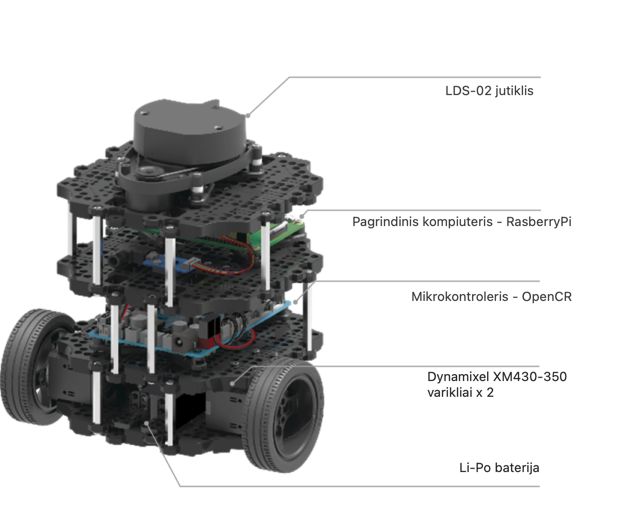
\includegraphics[width=0.7\textwidth]{images/TurtleBot.png}
    \caption{TurtleBot3 Burger roboto pagrindiniai komponentai}
    \label{fig:turtlebot-components}
\end{figure}

Roboto komponentų tarpusavio ryšiai pateikti \ref{fig:turtlebot-system-components} pav. Schema parodo, kaip atskiriami aukšto lygio skaičiavimai, žemo lygio
judėjimo valdymas, jutiklių duomenų gavimas ir roboto maitinimas.

\begin{figure}[H]
    \centering
    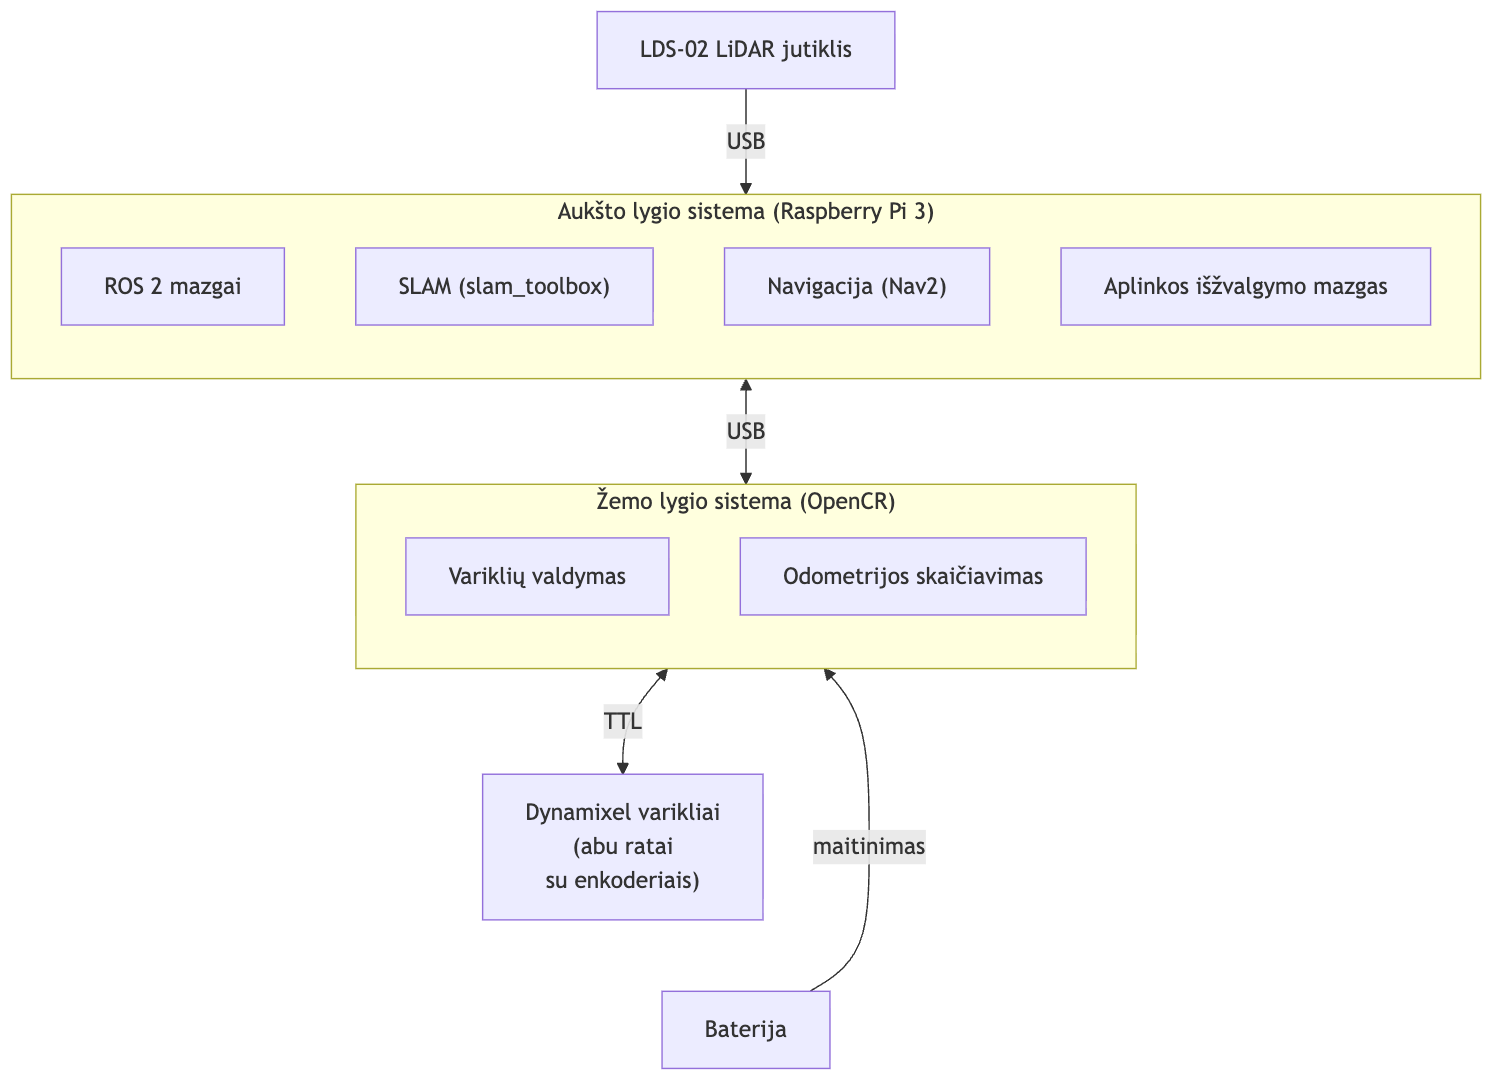
\includegraphics[width=0.7\textwidth]{images/diagramos/robot-komponent.png}
    \caption{TurtleBot Burger sistemos komponentų sąveika}
    \label{fig:turtlebot-system-components}
\end{figure}

Schema parodo pagrindinius duomenų ir valdymo ryšius: LDS-02 jutiklis USB sąsaja perduoda matavimus aukšto lygio sistemai, \textit{Raspberry Pi 3} ir
\textit{OpenCR} valdiklis tarpusavyje keičiasi duomenimis per USB, o \textit{OpenCR} per TTL (angl. \textit{Transistor-Transistor Logic}) sąsają valdo \textit{DYNAMIXEL} variklius. Tokia struktūra
atskiria skaičiavimams imlias navigacijos ir išžvalgymo užduotis nuo tiesioginio roboto judėjimo valdymo.

\subsection{Judėjimo sistema ir odometrija}

Roboto judėjimas realizuojamas naudojant diferencinio valdymo schemą. Šioje schemoje robotas turi du nepriklausomai valdomus varomuosius ratus. Keičiant
kairiojo ir dešiniojo rato greičius, robotas gali judėti tiesiai, suktis vietoje arba važiuoti lenkta trajektorija. Tokia važiuoklės konstrukcija yra paprasta
ir tinkama vidaus patalpoms, nes leidžia robotui manevruoti kambariuose, koridoriuose ir siauresniuose praėjimuose.

Kiekvieno rato judėjimui naudojami \textit{DYNAMIXEL} varikliai. Jie leidžia valdyti ratų sukimosi greitį ir gauti informaciją apie ratų judėjimą. Pagal
šią informaciją apskaičiuojama roboto odometrija, t. y. įvertinama, kaip robotas pajudėjo nuo ankstesnės padėties. Odometrijos duomenys ROS~2 sistemoje
naudojami roboto judėjimui sekti ir yra svarbūs SLAM algoritmui.

Vis dėlto odometrija realiomis sąlygomis nėra visiškai tiksli. Klaidos gali atsirasti dėl ratų praslydimo, grindų nelygumų, netolygaus paviršiaus arba
mechaninių paklaidų. Ilgesnio judėjimo metu šios klaidos kaupiasi, todėl vien odometrijos nepakanka patikimai roboto lokalizacijai. Dėl šios priežasties
odometrijos duomenys derinami su lazerinio jutiklio matavimais ir SLAM sistema, kuri nuolat atnaujina roboto padėtį sudaromame žemėlapyje.

\subsection{OpenCR mikrovaldiklio vaidmuo}

\textit{OpenCR} valdiklis šiame darbe naudojamas kaip standartinė \textit{TurtleBot3 Burger} žemo lygio valdymo dalis. Jis veikia kaip tarpinė grandis tarp
pagrindinio kompiuterio ir fizinių roboto komponentų. Per šį valdiklį vykdomas ryšys su \textit{DYNAMIXEL} varikliais, perduodami baziniai valdymo
signalai ir formuojami odometrijos duomenys.

Šiame darbe \textit{OpenCR} valdikliui naudojama oficiali \textit{TurtleBot3} programinė įranga. Atskiras žemo lygio valdymo kodas valdikliui nebuvo kuriamas,
nes darbo tikslas yra ne variklių valdymo ar mikrovaldiklio programavimo tyrimas, o aplinkos išžvalgymo algoritmų palyginimas. Standartinės programinės
įrangos naudojimas leidžia sumažinti papildomų kintamųjų skaičių eksperimentuose ir užtikrina, kad visi algoritmai veiktų su tuo pačiu baziniu roboto
valdymo sluoksniu.

\begin{figure}[H]
    \centering
    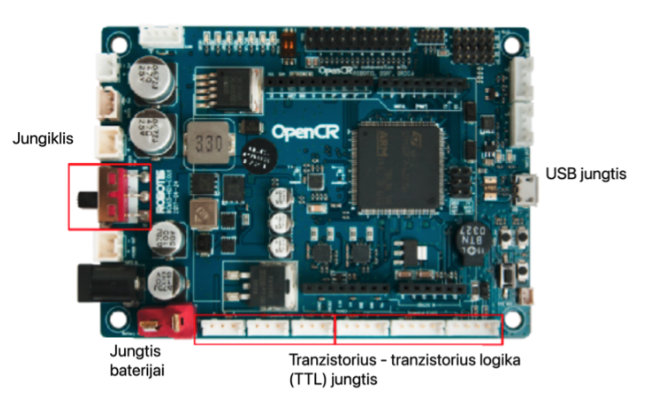
\includegraphics[width=0.9\textwidth]{images/OpenCR.png}
    \caption{OpenCR mikrovaldiklio elementai}
    \label{fig:opencr-elements}
\end{figure}

\subsection{Aukšto lygio skaičiavimo sistema}

Aukšto lygio programinei įrangai vykdyti naudojamas \textit{Raspberry Pi 3} mikrokompiuteris. Jis atlieka pagrindinio roboto kompiuterio vaidmenį.
Šiame kompiuteryje veikia operacinė sistema, ROS~2 Humble aplinka ir pagrindiniai programiniai komponentai, reikalingi roboto navigacijai ir aplinkos išžvalgymui.

\textit{Raspberry Pi 3} palaiko ryšį su \textit{OpenCR} valdikliu, priima odometrijos ir jutiklių duomenis, vykdo SLAM žemėlapio sudarymo procesą, Nav2
navigacijos komponentus ir aplinkos išžvalgymo mazgą. Tokia sistema leidžia robote vykdyti visą autonominio tyrinėjimo ciklą: nuo aplinkos skenavimo iki
naujo navigacijos tikslo parinkimo ir judėjimo iki jo.

Kadangi \textit{Raspberry Pi 3} \textbf{skaičiavimo ištekliai yra riboti}, sistemos konfigūracija turi būti parinkta taip, kad visi komponentai galėtų veikti realiuoju
laiku. Dėl šios priežasties žemėlapio rezoliucija, SLAM atnaujinimo dažnis, lazerinių duomenų apdorojimas ir išžvalgymo ciklo dažnis buvo derinami
atsižvelgiant į roboto kompiuterio pajėgumą. Tai ypač svarbu, nes vienu metu veikia keli skaičiavimams imlūs procesai: LiDAR duomenų perdavimas,
\textit{slam\_toolbox}, Nav2 ir aktyvus išžvalgymo algoritmas.

\subsection{Aplinkos jutiklių integracija}

Aplinkos suvokimui naudojamas \textbf{LDS-02 lazerinis atstumo jutiklis}. Šis jutiklis skenuoja aplinką horizontalioje plokštumoje ir pateikia atstumų matavimus iki
aplinkinių objektų. Gauti duomenys ROS~2 sistemoje naudojami žemėlapio sudarymui, kliūčių aptikimui ir navigacijos sistemos darbui.

LiDAR jutiklis yra vienas svarbiausių fizinės sistemos komponentų šiame darbe, nes aplinkos išžvalgymo algoritmai remiasi ne tiesioginiais lazerio
matavimais, o iš jų sudarytu užimtumo tinklu. SLAM sistema pagal lazerio ir odometrijos duomenis atnaujina žemėlapį, o algoritmai šiame žemėlapyje ieško
nežinomų sričių, ribų ir tinkamų navigacijos tikslų.

Darbe taip pat naudojamas atskiras LDS-02 jutiklio tvarkyklės mazgas. Jo paskirtis - per nuosekliąją sąsają, fiziškai prijungtą prie \textit{Raspberry Pi 3}
per USB jungtį, nuskaityti lazerinio jutiklio duomenis ir perduoti juos ROS~2 sistemai standartiniu formatu.
Realiuose eksperimentuose jutiklio duomenų kokybė turi tiesioginę įtaką žemėlapio tikslumui. Netikslūs arba nepilni matavimai gali lemti netiksliai pažymėtas
kliūtis, neištirtas sritis ar neteisingai aptiktas ribas. Todėl prieš eksperimentus buvo tikrinama, ar LDS-02 jutiklis stabiliai publikuoja duomenis, ar jie
pasiekia SLAM sistemą ir ar žemėlapis atnaujinamas pagal roboto judėjimą.

\subsection{Fizinės sistemos paruošimas eksperimentams}

Prieš atliekant eksperimentus fizinė roboto sistema buvo paruošiama taip, kad bandymai vyktų kuo stabilesnėmis sąlygomis. Buvo tikrinamas baterijos gyvavimo laikas, ryšys su \textit{Raspberry Pi 3}, \textit{OpenCR} mikrovaldiklio veikimas, variklių atsakas, odometrijos publikavimas, LiDAR duomenų gavimas ir
transformacijų medis.

Svarbi paruošimo dalis buvo patikrinti, ar ROS~2 sistemoje pasiekiamos pagrindinės temos. Odometrijos duomenys turėjo būti publikuojami \textit{/odom}
temoje, lazerio duomenys - \textit{/scan} temoje, o SLAM sistema turėjo publikuoti žemėlapį \textit{/map} temoje. Taip pat buvo tikrinama, ar transformacijos
tarp \textit{map}, \textit{odom} ir \textit{base\_footprint} koordinačių sistemų yra prieinamos ir atnaujinamos.

Eksperimentuose buvo svarbu, kad fizinė platforma visiems algoritmams būtų vienoda. Todėl roboto aparatinė konfigūracija tarp algoritmų nebuvo keičiama. Tokiu būdu siekta,
kad rezultatų skirtumai būtų susiję su algoritmų sprendimų priėmimu, o ne su fizinės sistemos pokyčiais.

\section[APLINKOS IŠŽVALGYMO SISTEMOS ARCHITEKTŪRA]{Aplinkos išžvalgymo sistemos architektūra}

Šiame skyriuje aprašoma sukurta aplinkos išžvalgymo sistema, kurioje įgyvendinami ir lyginami pasirinkti algoritmai. Sistemos paskirtis - sudaryti vienodas
sąlygas visiems algoritmams, tai leidžia palyginimą sieti su algoritmų sprendimų priėmimo principais, o ne su skirtingomis programinės įrangos
sąlygomis.

Sistema realizuota kaip ROS~2 paketas \textit{room\_exploration}. Jame apjungiamas \textit{TurtleBot Burger} roboto paleidimas, \textit{slam\_toolbox}
žemėlapio sudarymas, Nav2 navigacijos sistema ir atskiras aplinkos išžvalgymo mazgas. Išžvalgymo mazgas gauna roboto poziciją ir SLAM sudaromą užimtumo tinklą,
pagal pasirinktą algoritmą apskaičiuoja kitą navigacijos tikslą ir perduoda jį Nav2 sistemai. Nav2 atsakinga už kelio planavimą, kliūčių vengimą ir roboto
judėjimą iki nurodyto tikslo. Šių komponentų ryšiai ir pagrindiniai duomenų srautai pateikti \ref{fig:exploration-system-architecture} pav.

\begin{figure}[H]
    \centering
    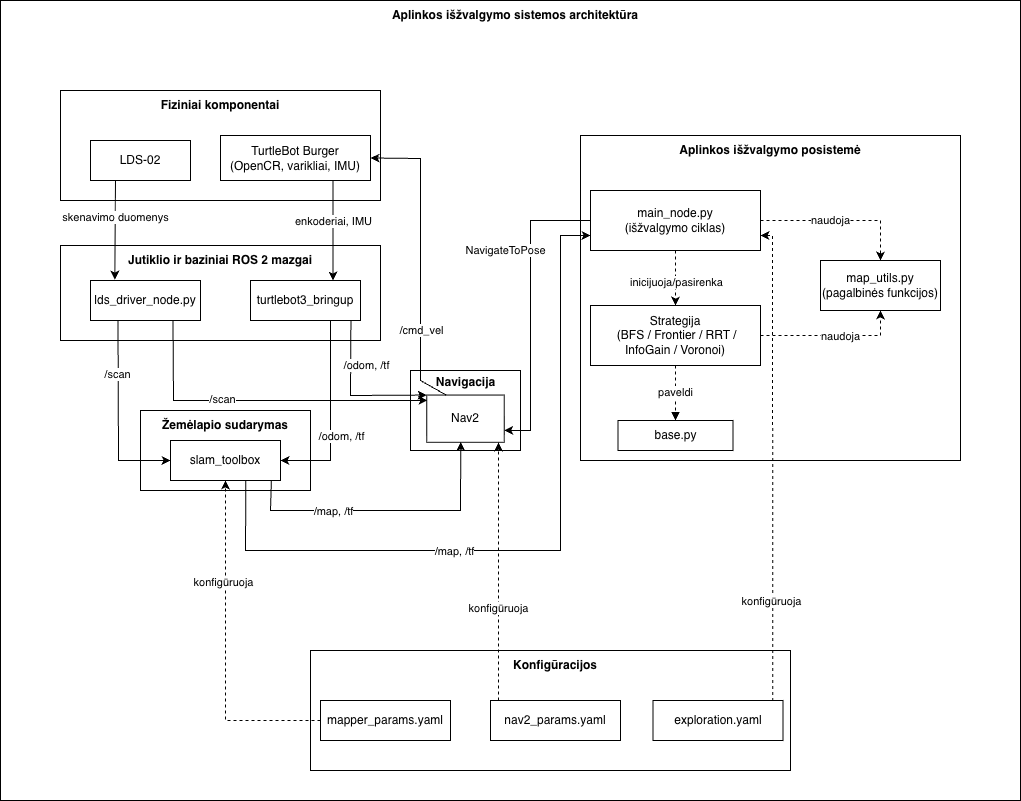
\includegraphics[width=0.95\textwidth]{images/diagramos/sysarch.png}
    \caption{Aplinkos išžvalgymo sistemos komponentų sąveika}
    \label{fig:exploration-system-architecture}
\end{figure}

Diagramoje matyti, kad LDS-02 jutiklio ir roboto bazės duomenys pirmiausia perduodami jutiklio bei baziniams ROS~2 mazgams. \textit{slam\_toolbox} naudoja lazerinio
skenavimo, odometrijos ir transformacijų duomenis žemėlapiui sudaryti, o išžvalgymo mazgas gauna žemėlapį bei roboto poziciją ir pagal pasirinktą strategiją
apskaičiuoja kitą navigacijos tikslą. Šis tikslas perduodamas Nav2 sistemai, kuri vykdo judėjimą ir grąžina rezultatą išžvalgymo ciklui. Vientisos rodyklės
žymi vykdymo metu perduodamus ROS~2 duomenis o punktyrinės rodyklės - konfigūravimo ryšius ir programines
priklausomybes tarp kodo modulių.

\subsection{Bendra sistemos struktūra}

Programinės sistemos architektūra sudaryta iš kelių pagrindinių ROS~2 dalių:
\begin{enumerate}
  \item jutiklio ir bazinių roboto ROS~2 mazgų, kurie publikuoja odometrijos, transformacijų ir lazerinio skenavimo duomenis;
  \item \textit{slam\_toolbox} mazgo, kuris pagal gaunamus duomenis sudaro užimtumo tinklą;
  \item Nav2 navigacijos sistemos, kuri vykdo judėjimą iki nurodyto tikslo;
  \item pagrindinio aplinkos išžvalgymo mazgo, kuris valdo išžvalgymo ciklą;
  \item penkių išžvalgymo strategijų, įgyvendintų per bendrą sąsają.
\end{enumerate}

Bendras sistemos veikimo principas remiasi uždaru išžvalgymo ciklu: SLAM sistema atnaujina žemėlapį, išžvalgymo mazgas pagal pasirinktą strategiją parenka
kitą navigacijos tikslą, o Nav2 vykdo roboto judėjimą iki šio tikslo. Pasiekus tikslą arba gavus nesėkmės būseną, ciklas kartojamas su atnaujintu užimtumo
tinklu.

\subsection{ROS 2 paketo struktūra}

Sukurta sistema realizuota ROS~2 darbo aplanke \textit{ros2\_ws}. Pagrindinis paketas vadinamas \textit{room\_exploration}. Visa šiame darbe naudota
programinio kodo bazė pateikiama \hyperref[priedas:kodo-saugykla]{1 priede}. Kodo bazėje galima rasti šiuos pagrindinius komponentus:
\begin{itemize}
  \item \textit{launch/bringup.launch.py} - šiame darbe sukurtas bendras paleidimo failas, paleidžiantis roboto, SLAM, Nav2 ir išžvalgymo mazgus;
  \item \textit{config/exploration.yaml} - išžvalgymo mazgo ir algoritmų parametrų failas;
  \item \textit{config/mapper\_params.yaml} - \textit{slam\_toolbox} konfigūracija;
  \item \textit{config/nav2\_params.yaml} - Nav2 navigacijos parametrų failas;
  \item \textit{room\_exploration/main\_node.py} - šiame darbe sukurtas pagrindinis išžvalgymo mazgas;
  \item \textit{room\_exploration/nodes/lds\_driver\_node.py} - šiame darbe sukurtas LDS-02 jutiklio tvarkyklės mazgas;
  \item \textit{room\_exploration/exploration/base.py} - šiame darbe sukurta bendra išžvalgymo algoritmų klasė;
  \item \textit{room\_exploration/exploration/bfs.py} - BFS algoritmo realizacija;
  \item \textit{room\_exploration/exploration/frontier.py} - artimiausios ribos algoritmo realizacija;
  \item \textit{room\_exploration/exploration/rrt.py} - RRT algoritmo realizacija;
  \item \textit{room\_exploration/exploration/information\_gain.py} - informacijos prieaugio algoritmo realizacija;
  \item \textit{room\_exploration/exploration/voronoi.py} - Voronoi diagramomis pagrįsto algoritmo realizacija;
  \item \textit{room\_exploration/map\_utils.py} - šiame darbe sukurtos bendros užimtumo tinklo apdorojimo funkcijos.
\end{itemize}

Tokia struktūra leidžia atskirti sistemos paleidimą, parametrus, bendrą išžvalgymo ciklą ir konkrečių algoritmų realizacijas. Tai palengvina algoritmų keitimą
ir leidžia skirtingus metodus paleisti naudojant tą patį pagrindinį mazgą.

\subsection{Sistemos paleidimo eiga}

Visa sistema paleidžiama naudojant šiame darbe sukurtą \textit{bringup.launch.py} failą. Paleidimo faile numatyta nuosekli mazgų paleidimo tvarka. Pirmiausia paleidžiamas
\textit{TurtleBot3} roboto valdymas, kuris inicijuoja roboto būsenos publikavimą, variklių valdymą, odometriją ir LiDAR duomenis. Po to paleidžiamas
\textit{slam\_toolbox} mazgas, kuris prenumeruoja \textit{/scan} duomenis ir publikuoja užimtumo tinklą temoje \textit{/map}. Vėliau paleidžiama Nav2
navigacijos sistema, o galiausiai paleidžiamas pagrindinis išžvalgymo mazgas.

Paleidimo faile naudojami laiko atidėjimai. Jie reikalingi tam, kad prieš paleidžiant SLAM ir navigaciją būtų stabiliai gaunami odometrijos bei transformacijų
duomenys. Tai svarbu realiame robote, nes sistemos paleidimo pradžioje jutikliai ir transformacijos dar gali būti nepasiruošę. Jei SLAM arba Nav2 būtų
paleisti per anksti, pirmieji duomenys galėtų būti atmesti arba žemėlapio sudarymas neprasidėtų stabiliai.

Paleidžiant sistemą galima nurodyti aktyvią išžvalgymo strategiją, tam naudojamas \textbf{\textit{strategy} argumentas}. Pavyzdžiui, galima paleisti BFS, artimiausios
ribos, RRT, informacijos prieaugio arba Voronoi pagrįstą algoritmą, nekeičiant pagrindinio kodo. Tai leidžia eksperimentų metu išlaikyti tą pačią sistemos
konfigūraciją ir keisti tik tiriamą algoritmą.

\subsection{SLAM ir žemėlapio sudarymas}

Žemėlapio sudarymui naudojamas \textit{slam\_toolbox}. Jis veikia žemėlapio sudarymo režimu ir pagal LiDAR skenavimo bei odometrijos duomenis kuria dvimatį
užimtumo tinklą. Užimtumo tinklo rezoliucija nustatyta į 0,05~m, todėl vienas tinklo langelis atitinka 5~cm realioje aplinkoje. Tokia rezoliucija yra
pakankama vidaus patalpų struktūrai, sienoms, objektams ir siauresniems praėjimams atvaizduoti, kartu išlaikant priimtiną skaičiavimo apkrovą.

\textit{slam\_toolbox} konfigūracijoje nurodomi koordinačių rėmų (angl. \textit{frame}) pavadinimai, pagal kuriuos SLAM mazgas susieja žemėlapį, odometriją ir
roboto padėtį. \textit{map} rėmas naudojamas sudaromam žemėlapiui, \textit{odom} rėmas - odometrijos duomenims, o \textit{base\_footprint} rėmas - roboto pagrindo padėčiai
aprašyti. LiDAR duomenys gaunami iš \textit{/scan} temos. Pagrindiniai \textit{mapper\_params.yaml} faile naudoti \textit{slam\_toolbox} parametrai pateikti
\ref{tab:slam-params} lentelėje.

\begin{table}[H]
\centering
\caption{\textit{slam\_toolbox} konfigūracijos parametrai}
\label{tab:slam-params}
\small
\begin{tabular}{|p{0.32\textwidth}|p{0.18\textwidth}|p{0.40\textwidth}|}
\hline
\textbf{Parametras} & \textbf{Reikšmė} & \textbf{Paskirtis} \\
\hline
\textit{mode} & \textit{mapping} & Žemėlapio sudarymo režimas. \\
\hline
\textit{map\_frame}, \textit{odom\_frame}, \textit{base\_frame} & \textit{map}, \textit{odom}, \textit{base\_footprint} & Koordinačių rėmai, susiejantys žemėlapį, odometriją ir roboto pagrindą. \\
\hline
\textit{scan\_topic} & \textit{/scan} & LiDAR skenavimo duomenų tema. \\
\hline
\textit{resolution} & 0,05~m & Užimtumo tinklo langelio dydis. \\
\hline
\textit{max\_laser\_range} & 3,5~m & Maksimalus lazerio matavimo nuotolis, naudojamas SLAM konfigūracijoje. \\
\hline
\textit{map\_update\_interval} & 1,5~s & Žemėlapio atnaujinimo intervalas. \\
\hline
\textit{transform\_publish\_period} & 0,10~s & Transformacijų publikavimo periodas. \\
\hline
\textit{minimum\_travel\_distance} & 0,01~m & Minimalus roboto poslinkis, po kurio vertinamas naujas skenavimas. \\
\hline
\textit{minimum\_travel\_heading} & 0,02~rad & Minimalus roboto pasisukimas, po kurio vertinamas naujas skenavimas. \\
\hline
\textit{scan\_queue\_size} & 10 & Skenavimų eilės dydis. \\
\hline
\textit{throttle\_scans} & 2 & Apdorojamas kas antras skenavimas, siekiant sumažinti skaičiavimo apkrovą. \\
\hline
\textit{use\_scan\_matching} & \textit{true} & Įjungtas skenavimų sutapatinimas roboto padėčiai tikslinti. \\
\hline
\textit{do\_loop\_closing} & \textit{false} & Ciklo uždarymas išjungtas, kad realiu laiku veikianti sistema mažiau apkrautų \textit{Raspberry Pi 3}. \\
\hline
\end{tabular}
\end{table}

SLAM mazgas publikuoja užimtumo tinklą temoje \textit{/map}. Šį žemėlapį naudoja tiek Nav2 navigacijos sistema, tiek išžvalgymo algoritmai.

\subsection{Nav2 navigacijos sistema}

Nav2 sistemos paskirtis šiame darbe yra vykdyti judėjimą iki išžvalgymo algoritmo parinkto tikslo. Kai išžvalgymo mazgas apskaičiuoja naują tikslą, jis
siunčiamas Nav2 veiksmų serveriui. Jei algoritmas grąžina vieną tikslą, naudojamas \textit{NavigateToPose} veiksmas. Jei algoritmas grąžina tarpinių taškų
seką, naudojamas \textit{NavigateThroughPoses} veiksmas. Tai leidžia palaikyti tiek vieno tikslo strategijas, tiek metodus, kuriems naudinga perduoti kelių
tarpinių taškų seką.

Visiems algoritmams naudojama ta pati Nav2 konfigūracija. Jei tikslas nepasiekiamas, Nav2 grąžina nesėkmės būseną, o išžvalgymo mazgas šį tikslą įtraukia į laikiną
nepasiekiamų tikslų sąrašą (angl. \textit{blacklist}). Tokiu būdu algoritmas gali bandyti pasirinkti kitą aplinkos sritį ir nekartoti to paties nepavykusio sprendimo.
Pagrindiniai \textit{nav2\_params.yaml} faile naudoti parametrai, turintys tiesioginę reikšmę judėjimui iki išžvalgymo algoritmo parinkto tikslo, pateikti
\ref{tab:nav2-params} lentelėje.

\begin{table}[H]
\centering
\caption{Nav2 konfigūracijos parametrai}
\label{tab:nav2-params}
\small
\begin{tabular}{|p{0.32\textwidth}|p{0.18\textwidth}|p{0.40\textwidth}|}
\hline
\textbf{Parametras} & \textbf{Reikšmė} & \textbf{Paskirtis} \\
\hline
\textit{controller\_frequency} & 5,0~Hz & Lokalaus valdiklio veikimo dažnis. \\
\hline
\textit{global\_frame}, \textit{robot\_base\_frame} & \textit{map}; \textit{base\_link} & Nav2 naudojami globalus ir roboto pagrindo koordinačių rėmai. \\
\hline
\textit{FollowPath.plugin} & \textit{RegulatedPurePursuitController} & Lokalus kelio sekimo valdiklis, pritaikantis greitį pagal kelią ir kliūtis. \\
\hline
\textit{desired\_linear\_vel}, \textit{rotate\_to\_heading\_angular\_vel} & 0,16~m/s; 0,8~rad/s & Pageidaujamas tiesinis greitis ir sukimosi greitis atsisukant į kryptį. \\
\hline
\textit{xy\_goal\_tolerance}, \textit{yaw\_goal\_tolerance} & 0,15~m; 3,14159~rad & Tikslo pasiekimui svarbiausia pozicija, o galutinė roboto orientacija beveik neribojama. \\
\hline
\textit{required\_movement\_radius}, \textit{movement\_time\_allowance} & 0,05~m; 15,0~s & Pažangos tikrinimo parametrai, naudojami nustatyti, ar robotas juda pakankamai. \\
\hline
\textit{robot\_radius}, \textit{footprint\_padding} & 0,105~m; 0,04~m & Roboto dydis ir papildomas saugos atstumas kliūčių žemėlapiuose. \\
\hline
\textit{inflation\_radius} & 0,22~m & Atstumas, kuriuo kliūčių įtaka išplečiama Nav2 kliūčių žemėlapiuose. \\
\hline
\textit{obstacle\_max\_range}, \textit{raytrace\_max\_range} & 3,0~m; 3,5~m & Kliūčių žymėjimo ir laisvos erdvės spindulio sekimo nuotoliai. \\
\hline
\textit{GridBased.plugin} & \textit{NavfnPlanner} & Globalus kelio planuotojas, sudarantis kelią iki nurodyto tikslo. \\
\hline
\textit{use\_astar}, \textit{allow\_unknown}, \textit{tolerance} & \textit{true}; \textit{true}; 0,25~m & Globalus kelias planuojamas A* paieška, leidžiant kelią per nežinomą sritį su nurodyta tikslo tolerancija. \\
\hline
\textit{behavior\_plugins} & \textit{spin}, \textit{backup}, \textit{wait} & Atkūrimo veiksmai, taikomi, kai navigacija nepavyksta iš karto. \\
\hline
\end{tabular}
\end{table}

\subsection{Pagrindinis išžvalgymo mazgas}

Pagrindinis sistemos komponentas yra \textit{ExplorationNode}, realizuotas faile \textit{main\_node.py}. Šis mazgas atlieka algoritmų orkestravimo funkciją.
Jis prenumeruoja SLAM publikuojamą žemėlapį, gauna roboto poziciją iš transformacijų medžio, siunčia tikslus Nav2 sistemai ir kaupia pagrindinius vykdymo
rodiklius.

Mazgas veikia baigtinio automato (angl. \textit{state machine}) principu. Sistemoje išskiriamos šios būsenos:
\begin{itemize}
  \item \textit{WAITING\_FOR\_DATA} - laukiama žemėlapio, transformacijų ir Nav2;
  \item \textit{COMPUTING\_GOAL} - skaičiuojamas kitas išžvalgymo tikslas;
  \item \textit{NAVIGATING} - tikslas išsiųstas Nav2 sistemai ir laukiama rezultato;
  \item \textit{GOAL\_REACHED} - tikslas pasiektas, galima skaičiuoti kitą tikslą;
  \item \textit{GOAL\_FAILED} - tikslo pasiekti nepavyko, reikia pasirinkti alternatyvą;
  \item \textit{COMPLETE} - išžvalgymo procesas baigtas.
\end{itemize}

Toks būsenų modelis leidžia aiškiai atskirti duomenų laukimą, tikslo skaičiavimą, navigacijos vykdymą ir eksperimento užbaigimą. Tai taip pat leidžia vienodai
tvarkyti visų algoritmų rezultatus: nepriklausomai nuo to, kokia strategija parenka tikslą, pagrindinis mazgas tą tikslą siunčia Nav2 sistemai ir registruoja
navigacijos baigtį.

Pagrindinis ciklas vykdomas nustatytu dažniu. Konfigūracijoje naudojamas 1~Hz dažnis, todėl išžvalgymo mazgas kartą per sekundę tikrina sistemos būseną,
jei reikia, skaičiuoja naują tikslą. Tikslui pasiekti taikomas laiko limitas. Jei robotas per nustatytą laiką nepasiekia tikslo,
tikslas laikomas nepavykusiu, o mazgas pereina į nesėkmės būseną.

\subsection{Bendroji algoritmų sąsaja}

Šiame darbe faile \textit{base.py} sukurta bendra klasė \textit{BaseExplorationStrategy}. Visi išžvalgymo algoritmai paveldi šią klasę. Ji apibrėžia bendrą sąsają, kurią turi įgyvendinti kiekviena
strategija. Pagrindinė funkcija yra \textbf{\textit{get\_next\_goal}}, kuri pagal užimtumo tinklą ir roboto poziciją grąžina kitą navigacijos tikslą. Taip pat numatyta
funkcija \textit{get\_next\_path}, kuri gali grąžinti kelių tarpinių tikslų seką. Pagal nutylėjimą ji apgaubia vieną tikslą į sąrašą, tačiau konkretus
algoritmas gali šią elgseną pakeisti.

Bendroje klasėje taip pat realizuotas tikslo validumo tikrinimas ir nepavykusių tikslų valdymas. Jei Nav2 nepavyksta pasiekti tikslo, jis įtraukiamas į
laikiną juodąjį sąrašą. Vėliau algoritmai gali vengti arti šių taškų esančių kandidatų. Tai reikalinga realiose patalpose, nes dėl kliūčių, siaurų praėjimų
arba netikslaus žemėlapio kai kurie tikslai gali atrodyti tinkami užimtumo tinkle, bet praktiškai būti nepasiekiami.

Bendros sąsajos naudojimas leidžia visus penkis algoritmus paleisti per tą patį pagrindinį mazgą. Tai mažina įgyvendinimo skirtumų poveikį eksperimentams ir
leidžia kiekvienam algoritmui naudoti tas pačias įvestis: užimtumo tinklą, roboto poziciją ir bendras pagalbines funkcijas.

\subsection{Užimtumo tinklo apdorojimo pagalbinės funkcijos}

Faile \textit{map\_utils.py} realizuotos funkcijos, kurios naudojamos visuose algoritmuose. Jos apima koordinačių konvertavimą tarp pasaulio koordinačių ir
užimtumo tinklo langelių, langelių klasifikavimą į laisvus, užimtus ir nežinomus, kaimyninių langelių gavimą, ribų aptikimą, ribos centro apskaičiavimą ir
žemėlapio padengimo įvertinimą.

Koordinačių konvertavimas yra būtinas todėl, kad algoritmai dažnai dirba su užimtumo tinklo langeliais, o Nav2 tikslai turi būti pateikiami metrais
\textit{map} koordinačių sistemoje. Todėl kandidatiniai langeliai turi būti paverčiami į pasaulio koordinates. Atvirkštinis konvertavimas reikalingas tada,
kai roboto pozicija arba kandidatinis taškas turi būti patikrintas užimtumo tinkle.

Ribų aptikimo funkcija identifikuoja laisvus langelius, esančius šalia nežinomų langelių, ir sugrupuoja juos į susijusias sritis. Ši funkcija naudojama
artimiausios ribos, informacijos prieaugio ir Voronoi strategijose. Bendras ribų aptikimo mechanizmas padeda užtikrinti, kad algoritmai naudotų tą pačią
pradinę ribų informaciją, o skirtumai atsirastų dėl skirtingo kandidatų vertinimo.

\subsection{LDS-02 jutiklio tvarkyklės mazgas}

Šiame darbe taip pat sukurtas LDS-02 lazerinio jutiklio tvarkyklės mazgas, realizuotas faile \textit{lds\_driver\_node.py}. Jo paskirtis - nuskaityti jutiklio
duomenis per nuosekliąją jungtį ir paversti juos standartiniu ROS~2 \textit{LaserScan} pranešimu, kurį gali naudoti \textit{slam\_toolbox} ir Nav2
komponentai. Tokia realizacija leidžia integruoti LDS-02 jutiklį į bendrą ROS~2 sistemą.

Tvarkyklės mazgas jungiasi prie jutiklio per \textit{/dev/ttyUSB0} jungtį 115200 duomenų perdavimo sparta. Gauti baitai kaupiami buferyje, kuriame ieškoma LDS-02
paketo pradžios antraštės. Aptikus pilną paketą, iš jo išskiriami pradinis ir galinis kampai, atstumų matavimai bei patikimumo reikšmės. Matavimai, kurie
neatitinka minimalaus atstumo arba patikimumo slenksčio, atmetami. Sukaupus pakankamą paketų skaičių vienam apsisukimui, sudaromas \textit{LaserScan}
pranešimas ir publikuojamas į \textit{/scan} temą.

Tai yra svarbi sukurtos sistemos dalis. Nuo stabilaus lazerinio jutiklio duomenų publikavimo priklauso
SLAM sudaromas užimtumo tinklas, o kartu ir visi vėlesni išžvalgymo algoritmų sprendimai.

\subsection{Parametrų konfigūracija}

Išžvalgymo mazgo ir algoritmų parametrai saugomi faile \textit{exploration.yaml}. Bendrieji parametrai apima ciklo dažnį, tikslo vykdymo laiko limitą, laukimo
laiką po nesėkmingo tikslo ir bandymų be naujo tikslo limitą. Atskirai pateikiami kiekvieno algoritmo parametrai, pavyzdžiui,
minimalus ribos dydis, minimalus tikslo atstumas, kliūčių atstumo reikalavimai, RRT iteracijų skaičius, informacijos vertinimo spindulys ar Voronoi keterų
(angl. \textit{ridge}) atstumo reikalavimai. Konkrečios kiekvieno algoritmo parametrų reikšmės ir jų įtaka algoritmo veikimui plačiau aprašomos 4 skyriuje.

Parametrų atskyrimas nuo programinio kodo leidžia eksperimentų metu keisti algoritmo elgseną nekeičiant realizacijos. Tačiau palyginimo metu svarbu išlaikyti
nuoseklią konfigūraciją ir taikyti vienodus principus visiems bandymams. Todėl bendri parametrai, tokie kaip navigacijos sąsaja, SLAM rezoliucija ir
pagrindinis išžvalgymo ciklas, išlaikomi tie patys visiems algoritmams.

\subsection{Rezultatų apskaičiavimas}

Eksperimento metu pagrindinis išžvalgymo mazgas kaupia pagrindinius rodiklius, reikalingus algoritmų palyginimui: \textbf{išžvalgymo trukmę, žemėlapio padengimą,
nuvažiuotą kelią ir išsiųstų tikslų skaičių (pavykusių ir nepavykusių)}. Šie rodikliai apskaičiuojami vykdymo metu ir pateikiami eksperimento pabaigoje kaip galutinė bandymo suvestinė.

Išžvalgymo trukmė skaičiuojama nuo išžvalgymo proceso pradžios iki eksperimento pabaigos. Žemėlapio padengimas apskaičiuojamas pagal SLAM sudaromą užimtumo
tinklą, naudojant \textit{compute\_coverage} funkciją. Ši funkcija skaičiuoja, kokia patalpos viduje esančios srities dalis yra pažymėta kaip žinoma.
Nežinoma erdvė, kuri lieka už sudaryto žemėlapio kraštų, į padengimo procentą neįtraukiama.

Žemėlapio padengimas apskaičiuojamas pagal formulę:
\begin{equation}
C = \frac{N_{\text{žinoma}}}{N_{\text{vidinė}}} \cdot 100~\%,
\end{equation}
čia $C$ yra žemėlapio padengimas procentais, $N_{\text{žinoma}}$ - žinomų laisvų arba užimtų langelių skaičius vertinamoje patalpos srityje, o
$N_{\text{vidinė}}$ - bendras vertinamos vidinės patalpos srities langelių skaičius.
Šios metrikos ribojimas yra tai, kad patalpos viduje esantys objektai gali sudaryti nežinomų langelių sritis užimtumo tinkle, todėl padengimo procentas gali
būti mažesnis net tada, kai robotas išžvalgo pasiekiamą patalpos dalį.
Kadangi užimtumo tinklas yra stačiakampis ir gali būti didesnis už vertinamą patalpą, jame gali būti langelių, kurie nepriklauso realiai vertinamai patalpos
sričiai. Todėl padengimo skaičiavime turi būti neįtraukiamos išorinės nežinomos sritys. Nors patalpose esantys objektai gali sumažinti galutinį padengimo procentą, ši
metrika išlieka tinkama algoritmų palyginimui, nes visi algoritmai vertinami tose pačiose aplinkose ir pagal tą patį skaičiavimo principą.

Nuvažiuotas kelias apskaičiuojamas pagal roboto pozicijos pokyčius odometrijos koordinačių sistemoje. Kiekvieną kartą gavus naują odometrijos pranešimą,
apskaičiuojamas atstumas tarp ankstesnės ir dabartinės roboto padėties, o šis atstumas pridedamas prie bendro kelio ilgio. Toks skaičiavimas leidžia įvertinti,
kiek fiziškai judėjo robotas vykdydamas konkretaus algoritmo parinktus navigacijos tikslus.

\subsection{Skyriaus apibendrinimas}

Sukurta sistema sudaro tinkamą eksperimentinę architektūrą aplinkos išžvalgymo algoritmams palyginti. Visi algoritmai naudoja tą patį \textit{TurtleBot
Burger} robotą, tą patį \textit{slam\_toolbox} sudaromą užimtumo tinklą, tą pačią Nav2 navigacijos sistemą ir tuos pačius rezultatų apskaičiavimo principus.
Skirtingi algoritmai įgyvendinti kaip atskiros strategijos, paveldinčios bendrą sąsają ir integruojamos į tą patį pagrindinį išžvalgymo mazgą.

Toks architektūrinis sprendimas leidžia izoliuoti pagrindinį tiriamą veiksnį - išžvalgymo tikslo parinkimo algoritmą. Tolimesniame skyriuje aprašomos
konkrečios šiame darbe įgyvendintos strategijos.


\section[APLINKOS IŠŽVALGYMO ALGORITMAI]{Aplinkos išžvalgymo algoritmai}

Šiame skyriuje aprašomi penki darbe įgyvendinti aplinkos išžvalgymo algoritmai. Algoritmų paskirtis yra parinkti \textbf{kitą
navigacijos tikslą}.

\subsection{Bendri algoritmų įgyvendinimo principai}

Visi algoritmai dirba su užimtumo tinklu, kuriame kiekvienas langelis gali būti nežinomas, laisvas arba užimtas. Nežinomi langeliai atitinka dar neištirtą
aplinkos dalį, laisvi langeliai žymi robotui pravažiuojamą erdvę, o užimti langeliai žymi kliūtis arba sienas. Praktiniame įgyvendinime laisvais laikomi
langeliai, kurių užimtumo reikšmė yra mažesnė už pasirinktą slenkstinę reikšmę, o nežinomi langeliai žymimi reikšme $-1$.

Daugelyje algoritmų naudojama ribos sąvoka. Šiame darbe riba vadinama žinomos laisvos srities ir nežinomos srities susidūrimo vieta. Praktiškai ribinis langelis yra
laisvas užimtumo tinklo langelis, kuris turi bent vieną nežinomą kaimyninį langelį. Tokie langeliai grupuojami į susijusias ribų sritis, o kiekvienai sričiai
gali būti apskaičiuojamas reprezentacinis taškas.

Kad robotas nebūtų siunčiamas į akivaizdžiai netinkamus tikslus, algoritmuose taikomi keli \textbf{bendri filtravimo principai}. Kandidatinis tikslas turi būti ne per
arti dabartinės roboto pozicijos, neturi būti įtrauktas į nepavykusių tikslų sąrašą ir turi tenkinti minimalų atstumą nuo kliūčių. Jei Nav2 sistemai nepavyksta
pasiekti pasirinkto tikslo, šis tikslas įtraukiamas į juodąjį sąrašą. Vėlesniuose cikluose algoritmai vengia kandidatų, esančių arti tokių nepavykusių tikslų.
Minimalus atstumas nuo roboto naudojamas tam, kad nebūtų pasirenkami beveik toje pačioje vietoje esantys tikslai, kurie mažai praplečia žemėlapį. Nepavykusių
tikslų sąrašas padeda išvengti pakartotinio roboto siuntimo į tą pačią probleminę vietą. Atstumas nuo kliūčių tikrinamas užimtumo tinkle: kandidatas atmetamas,
jei nustatytu spinduliu aplink jį yra užimtų langelių. Taip sumažinama tikimybė pasirinkti tikslą prie pat sienos, objekto arba siauro praėjimo krašto.

Bendrieji parametrų pasirinkimo principai buvo susiję su roboto matmenimis, užimtumo tinklo rezoliucija ir realių bandymų metu pastebėtu navigacijos tikslų
pasiekiamumu. Užimtumo tinklo rezoliucija buvo 0,05~m, todėl langeliais išreikšti parametrai gali būti tiesiogiai siejami su realiais atstumais. Bendras
minimalus tikslo atstumas daugumoje algoritmų buvo 0,3~m. Tokia reikšmė pasirinkta todėl, kad ji yra pakankama atmesti labai artimus ir mažai naudingus tikslus,
tačiau dar nėra per didelė siauresnėms patalpos vietoms ar praėjimams. Informacijos vertinimui naudotas 3,5~m atstumas, atitinkantis šiame darbe naudotą LDS-02
jutiklio naudingą veikimo nuotolį. Kiti parametrai parinkti taip, kad nebūtų atmetamos siauros ribos ir praėjimai, bet kartu būtų sumažinta rizika siųsti
robotą į per arti kliūčių esančius taškus.

\subsection{BFS algoritmas}

\textbf{BFS tipo algoritmas} remiasi paieška į plotį per žinomą laisvą užimtumo tinklo dalį. Paieška pradedama nuo roboto poziciją atitinkančio
langelio. Toliau plečiama per laisvus kaimyninius langelius, kol randamas tinkamas ribinis langelis. Tokiu būdu algoritmas pirmiausia aptinka ribas, kurios
yra pasiekiamos per žinomą laisvą erdvę.

Šiame darbe BFS algoritmas įgyvendintas taip, kad jis neplanuotų galutinio roboto kelio, o tik parinktų kitą navigacijos tikslą. Algoritmas naudoja 4 kaimynų plėtimą, nes toks plėtimas mažina riziką pasirinkti tikslus, kurie teoriškai pasiekiami tik įstrižai
tarp dviejų kliūčių kampų, bet realiai Nav2 planuotojui gali būti nepasiekiami.

BFS algoritmas tikrina, ar rastas ribinis langelis atitinka kelias sąlygas. Pirma, tikslas turi būti pakankamu atstumu nuo roboto. Antra, aplink tikslą turi
būti pakankamai laisvos vietos. Trečia, riba turi būti ne mažesnė už minimalų nustatytą dydį, kad robotas nebūtų siunčiamas į labai mažus triukšmingus
žemėlapio fragmentus. Jei visi kriterijai tenkinami, ribinis langelis konvertuojamas į pasaulio koordinates ir grąžinamas kaip navigacijos tikslas.

Siekiant sumažinti riziką siųsti robotą tiesiai į nežinomos srities kraštą, BFS realizacijoje naudojamas \textit{goal\_standoff\_cells} parametras. Jis
leidžia tikslą perkelti keliais BFS kelio žingsniais atgal nuo ribos į žinomą laisvą erdvę. Tai padidina tikimybę, kad Nav2 galės saugiai suplanuoti kelią iki
tikslo.

BFS algoritmo parametrai parinkti taip, kad metodas išliktų jautrus net mažoms riboms, bet kartu nesiųstų roboto į per arti kliūčių arba per arti dabartinės
pozicijos esančius taškus. Kadangi BFS paieška pirmą tinkamą ribą randa sistemingai judėdama per laisvą sritį, tikslas papildomai atitraukiamas nuo ribos į
žinomą erdvę. Taip sumažinama rizika, kad navigacijos tikslas pateks tiesiai ant nežinomos srities krašto. BFS algoritmo naudojami parametrai pateikti
\ref{tab:bfs-pseudocode-params} lentelėje.

\begin{table}[H]
\centering
\caption{BFS algoritmo naudojami parametrai}
\label{tab:bfs-pseudocode-params}
\small
\begin{tabular}{|p{1.8cm}|p{3.8cm}|p{2.1cm}|p{6.2cm}|}
\hline
\textbf{Žymėjimas} & \textbf{Parametras} & \textbf{Reikšmė} & \textbf{Paskirtis} \\
\hline
$d_{\min}$ & \textit{min\_goal\_distance} & 0,3~m & Mažiausias leidžiamas atstumas tarp roboto ir naujo tikslo. \\
\hline
$c$ & \textit{clearance\_cells} & 1 & Kiek užimtumo tinklo langelių aplink kandidatinį tikslą turi būti be kliūčių. \\
\hline
$s$ & \textit{goal\_standoff\_cells} & 2 & Kiek BFS kelio žingsnių tikslas atitraukiamas nuo ribos į žinomą laisvą sritį. \\
\hline
$f_{\min}$ & \textit{min\_frontier\_size} & 1 & Mažiausias leidžiamas ribos dydis langeliais. \\
\hline
\end{tabular}
\end{table}

\begin{algorithm}[H]
\caption{BFS}
\begin{algorithmic}[1]
\STATE \textbf{Duodama:} užimtumo tinklas $M$, roboto pozicija $p_r$, parametrai $d_{\min}$, $c$, $s$, $f_{\min}$
\STATE \textbf{Grąžinama:} navigacijos tikslas $g$ arba \textit{None}
\STATE $r \leftarrow \mathrm{WorldToGrid}(p_r, M)$
\STATE $Q \leftarrow [r]$
\STATE $V \leftarrow \emptyset$
\WHILE{$Q \neq [\ ]$}
  \STATE $u \leftarrow Q.\mathrm{PopFirst}()$
  \IF{$u \in V$}
    \STATE \textbf{continue}
  \ENDIF
  \STATE $V \leftarrow V \cup \{u\}$
  \IF{$\neg \mathrm{IsFree}(M,u)$}
    \STATE \textbf{continue}
  \ENDIF
  \IF{$\mathrm{HasUnknownNeighbor}(M,u)$}
    \STATE $f \leftarrow \mathrm{FrontierCluster}(M,u)$
    \IF{$|f| < f_{\min}$}
      \STATE \textbf{continue}
    \ENDIF
    \STATE $q \leftarrow \mathrm{MoveBackFromFrontier}(u,s)$
    \STATE $g \leftarrow \mathrm{GridToWorld}(q,M)$
    \IF{$\mathrm{Distance}(p_r,g) \geq d_{\min}$ \AND $\neg \mathrm{IsBlacklisted}(g)$ \AND $\mathrm{HasObstacleClearance}(M,q,c)$}
      \RETURN $g$
    \ENDIF
  \ENDIF
  \FORALL{$v \in \mathrm{Neighbors4}(u)$}
    \IF{$v \notin V$ \AND $\mathrm{IsFree}(M,v)$}
      \STATE $Q.\mathrm{Append}(v)$
    \ENDIF
  \ENDFOR
\ENDWHILE
\RETURN \textit{None}
\end{algorithmic}
\end{algorithm}

\subsection{Artimiausios ribos algoritmas}

\textbf{Artimiausios ribos algoritmas} yra klasikinio ribomis pagrįsto išžvalgymo realizacija. Pirmiausia iš užimtumo tinklo aptinkamos visos ribinės sritys. Tada
kiekvienai ribai apskaičiuojamas reprezentacinis taškas, naudojant ribos langelių centroidę. Jei centroidė patenka į netinkamą langelį, parenkamas
artimiausias tinkamas tos ribos langelis.

Po ribų aptikimo algoritmas atmeta netinkamus kandidatus. Nevertinamos per mažos ribos, per arti roboto esantys tikslai, tikslai be pakankamo atstumo nuo
kliūčių ir tikslai, esantys arti anksčiau nepavykusių navigacijos taškų. Iš likusių kandidatų pasirenkama riba, kurios reprezentacinis taškas yra arčiausiai
dabartinės roboto pozicijos pagal Euklido atstumą.

Šis metodas yra paprastas ir dažnai efektyvus atvirose arba mažiau sudėtingose patalpose. Jo pagrindinis privalumas yra mažas sprendimo sudėtingumas ir aiški
logika: robotas juda į artimiausią dar neištirtą aplinkos dalį. Tačiau metodas gali būti trumparegiškas. Artimiausia riba nebūtinai suteikia daugiausia naujos
informacijos, o sudėtingesnėje patalpoje toks pasirinkimas gali lemti papildomą grįžimą arba mažiau efektyvų aplinkos padengimą.

Artimiausios ribos algoritmo parametrai parinkti kaip kompromisas tarp ribų filtravimo ir gebėjimo reaguoti į nedideles, bet svarbias ribas. Per maži ribų
fragmentai gali atsirasti dėl žemėlapio netikslumų, todėl jie atmetami, tačiau riba neturi būti reikalaujama per didelė, nes siauruose praėjimuose ir prie durų
naudingi ribiniai fragmentai gali būti nedideli. Artimiausios ribos algoritmo naudojami parametrai pateikti \ref{tab:frontier-pseudocode-params} lentelėje.

\begin{table}[H]
\centering
\caption{Artimiausios ribos algoritmo naudojami parametrai}
\label{tab:frontier-pseudocode-params}
\small
\begin{tabular}{|p{1.8cm}|p{3.8cm}|p{2.1cm}|p{6.2cm}|}
\hline
\textbf{Žymėjimas} & \textbf{Parametras} & \textbf{Reikšmė} & \textbf{Paskirtis} \\
\hline
$d_{\min}$ & \textit{min\_goal\_distance} & 0,3~m & Mažiausias leidžiamas atstumas tarp roboto ir ribos reprezentacinio taško. \\
\hline
$c$ & \textit{clearance\_cells} & 2 & Kiek užimtumo tinklo langelių aplink kandidatinį tikslą turi būti be kliūčių. \\
\hline
$f_{\min}$ & \textit{min\_frontier\_size} & 3 & Mažiausias leidžiamas ribos dydis langeliais. \\
\hline
\end{tabular}
\end{table}

\begin{algorithm}[H]
\caption{Artimiausios ribos algoritmas}
\begin{algorithmic}[1]
\STATE \textbf{Duodama:} užimtumo tinklas $M$, roboto pozicija $p_r$, parametrai $d_{\min}$, $c$, $f_{\min}$
\STATE \textbf{Grąžinama:} navigacijos tikslas $g$ arba \textit{None}
\STATE $F \leftarrow \mathrm{DetectFrontiers}(M,f_{\min})$
\STATE $K \leftarrow [\ ]$
\FORALL{$f \in F$}
  \STATE $q \leftarrow \mathrm{FrontierCentroid}(f,M)$
  \IF{$\neg \mathrm{IsFree}(M,q)$}
    \STATE $q \leftarrow \mathrm{NearestFrontierCell}(f,q)$
  \ENDIF
  \STATE $g \leftarrow \mathrm{GridToWorld}(q,M)$
  \IF{$\mathrm{Distance}(p_r,g) < d_{\min}$}
    \STATE \textbf{continue}
  \ENDIF
  \IF{$\mathrm{IsBlacklisted}(g)$}
    \STATE \textbf{continue}
  \ENDIF
  \IF{$\neg \mathrm{HasObstacleClearance}(M,q,c)$}
    \STATE \textbf{continue}
  \ENDIF
  \STATE $K.\mathrm{Append}(g)$
\ENDFOR
\IF{$K = [\ ]$}
  \RETURN \textit{None}
\ENDIF
\STATE $g \leftarrow \arg\min_{g \in K} \mathrm{Distance}(p_r,g)$
\RETURN $g$
\end{algorithmic}
\end{algorithm}

\subsection{RRT algoritmas}

\textbf{RRT algoritmas} remiasi atsitiktine imtimi ir medžio augimu. Pradinė medžio viršūnė yra dabartinė roboto pozicija. Kiekvienos iteracijos metu algoritmas
pasirenka atsitiktinį tašką žemėlapio ribose, randa artimiausią esamą medžio viršūnę ir bando pratęsti medį link pasirinkto taško nustatytu žingsnio dydžiu.
Jei naujas taškas yra žinomoje laisvoje erdvėje ir atkarpa iki jo nekerta kliūčių, taškas įtraukiamas į medį.

Kiekvienoje RRT iteracijoje pasirenkamas vienas imties taškas. Su \textit{goal\_bias} parametru nurodyta tikimybe algoritmas pirmiausia bando parinkti tašką iš
nežinomos užimtumo tinklo srities. Jei tokio taško rasti nepavyksta arba jei ši tikimybė nesuveikia, imtis parenkama atsitiktinai visose žemėlapio ribose. Taip
RRT medis dažniau nukreipiamas į neištirtas sritis, tačiau algoritmas nepraranda bendro atsitiktinio žemėlapio tyrinėjimo principo. Jei naujas medžio taškas
ribojasi su nežinomais langeliais, jis laikomas kandidatu išžvalgymo tikslui. Kandidatai taip pat tikrinami pagal minimalų atstumą nuo roboto ir kliūčių
atstumo reikalavimus.

RRT algoritmas gali rasti kandidatus skirtingose žemėlapio dalyse ir nėra apribotas vien sistemingu ribų skenavimu. Tai leidžia metodui veikti kaip imtimi
pagrįstai išžvalgymo strategijai. Tačiau dėl atsitiktinės prigimties algoritmas gali būti mažiau stabilus siauruose praėjimuose arba aplinkose, kur svarbi
riba yra sunkiai pasiekiama atsitiktiniu medžio augimu.

Šio darbo realizacijoje iš visų rastų RRT kandidatų pasirenkamas tas, kurio naudingumo įvertis yra didžiausias. Naudingumas skaičiuojamas kaip stebimų
nežinomų langelių skaičiaus ir kelio medžiu kainos derinys:

\begin{equation}
S = I - w \cdot C,
\end{equation}

čia $I$ yra nežinomų langelių skaičius, kurį algoritmas įvertina kaip galimą atskleisti iš kandidatinio taško, $C$ - kelio kaina nuo roboto pozicijos iki
kandidato per RRT medį, o $w$ - kainos svoris. Tokiu būdu
algoritmas ne tik ieško ribinių taškų, bet ir bando derinti informacijos kiekį su judėjimo kaina.

RRT algoritmo parametrai parinkti siekiant išlaikyti balansą tarp atsitiktinės paieškos aprėpties ir skaičiavimo trukmės. Iteracijų skaičius riboja, kiek
ilgai viename cikle leidžiama plėsti medį, o žingsnio dydis lemia, kaip greitai medis plečiasi per žinomą laisvą erdvę. Nedidelė imties nukreipimo į nežinomą
sritį tikimybė padeda dažniau auginti medį tyrinėjimo kryptimi, bet nepašalina atsitiktinės paieškos savybės. RRT algoritmo naudojami parametrai pateikti
\ref{tab:rrt-pseudocode-params} lentelėje.

\begin{table}[H]
\centering
\caption{RRT algoritmo naudojami parametrai}
\label{tab:rrt-pseudocode-params}
\small
\begin{tabular}{|p{1.8cm}|p{3.8cm}|p{2.1cm}|p{6.2cm}|}
\hline
\textbf{Žymėjimas} & \textbf{Parametras} & \textbf{Reikšmė} & \textbf{Paskirtis} \\
\hline
$N$ & \textit{max\_iterations} & 250 & Didžiausias RRT medžio plėtimo iteracijų skaičius viename tikslo paieškos cikle. \\
\hline
$\Delta$ & \textit{step\_size} & 0,4~m & Medžio plėtimo žingsnis nuo artimiausios viršūnės link imties taško. \\
\hline
$b$ & \textit{goal\_bias} & 0,1 & Tikimybė imtį nukreipti į nežinomą sritį. \\
\hline
$R$ & \textit{sensor\_range} & 3,5~m & Spindulys, kuriame vertinamas galimas nežinomų langelių atskleidimas. \\
\hline
$w$ & \textit{cost\_weight} & 1,0 & Kelio kainos svoris kandidato įvertyje. \\
\hline
$d_{\min}$ & \textit{min\_goal\_distance} & 0,3~m & Mažiausias leidžiamas atstumas tarp roboto ir kandidatinio tikslo. \\
\hline
$c$ & \textit{clearance\_cells} & 2 & Kiek užimtumo tinklo langelių aplink kandidatinį tikslą turi būti be kliūčių. \\
\hline
\end{tabular}
\end{table}

\begin{algorithm}[H]
\caption{RRT}
\begin{algorithmic}[1]
\STATE \textbf{Duodama:} užimtumo tinklas $M$, roboto pozicija $p_r$, parametrai $N$, $\Delta$, $b$, $R$, $w$, $d_{\min}$, $c$
\STATE \textbf{Grąžinama:} navigacijos tikslas $g$ arba \textit{None}
\STATE $T \leftarrow \mathrm{Tree}(p_r)$
\STATE $K \leftarrow [\ ]$
\FOR{$i \leftarrow 1$ \TO $N$}
  \IF{$\mathrm{Random}() < b$}
    \STATE $s \leftarrow \mathrm{SampleUnknownCell}(M)$
  \ELSE
    \STATE $s \leftarrow \mathrm{SampleMapCell}(M)$
  \ENDIF
  \IF{$s = \mathrm{None}$}
    \STATE \textbf{continue}
  \ENDIF
  \STATE $v \leftarrow \mathrm{NearestVertex}(T,s)$
  \STATE $n \leftarrow \mathrm{Steer}(v,s,\Delta)$
  \IF{$\neg \mathrm{IsFree}(M,n)$ \OR $\mathrm{LineHitsObstacle}(M,v,n)$}
    \STATE \textbf{continue}
  \ENDIF
  \STATE $T.\mathrm{AddVertex}(n,v)$
  \IF{$\mathrm{HasUnknownNeighbor}(M,n)$ \AND $\mathrm{Distance}(p_r,n) \geq d_{\min}$ \AND $\mathrm{HasObstacleClearance}(M,n,c)$}
    \STATE $K.\mathrm{Append}(n)$
  \ENDIF
\ENDFOR
\IF{$K = [\ ]$}
  \RETURN \textit{None}
\ENDIF
\STATE $bestScore \leftarrow -\infty$
\STATE $g_{best} \leftarrow \mathrm{None}$
\FORALL{$k \in K$}
  \STATE $I \leftarrow \mathrm{ObservableUnknownCount}(M,k,R)$
  \STATE $C \leftarrow \mathrm{TreePathCost}(T,k)$
  \STATE $S \leftarrow I - w \cdot C$
  \IF{$S > bestScore$}
    \STATE $bestScore \leftarrow S$
    \STATE $g_{best} \leftarrow \mathrm{GridToWorld}(k,M)$
  \ENDIF
\ENDFOR
\RETURN $g_{best}$
\end{algorithmic}
\end{algorithm}

\subsection{Informacijos prieaugio algoritmas}

\textbf{Informacijos prieaugio algoritmas} taip pat remiasi ribų aptikimu, tačiau ribos pasirenkamos ne vien pagal atstumą. Pirmiausia aptinkamos visos ribinės sritys,
kiekvienai apskaičiuojamas reprezentacinis taškas, o tada kiekvienas kandidatas įvertinamas pagal potencialiai gaunamos informacijos kiekį ir atstumą nuo
roboto.

Informacijos prieaugis šiame darbe skaičiuojamas nuo kandidatinio tikslo atliekant paiešką į plotį užimtumo tinkle. Paieška plečiama į kaimyninius langelius
ir skaičiuoja, kiek nežinomos srities galėtų būti atskleista robotui nuvykus į pasirinktą tikslą. Paieška ribojama pagal LDS-02 jutiklio veikimo
atstumą, kuris šiame darbe nustatytas į 3,5~m. Per užimtus langelius paieška neplečiama, todėl sienos ir kliūtys riboja skaičiuojamą informacijos prieaugį.

Nors literatūroje informacijos prieaugis dažnai siejamas su entropijos arba žemėlapio neapibrėžtumo mažėjimo skaičiavimu, šiame darbe pasirinkta paprastesnė
praktinė realizacija. Ji skiriasi nuo literatūros analizėje pateiktos entropija paremtos formulės, nes čia siekiama ne prognozuoti tikslų būsimo žemėlapio
neapibrėžtumo pokytį, o praktiškai palyginti kandidatinius tikslus. Algoritmas neskaičiuoja, ką robotas tikrai pamatys nuvykęs į tikslą, o įvertina, kiek
nežinomų užimtumo tinklo langelių pagal dabartinį žemėlapį galėtų būti atskleista iš kandidatinio tikslo.

Kad algoritmas nepasirinktų labai tolimų tikslų vien dėl didelio nežinomų langelių skaičiaus, naudojamas kombinuotas įvertis. Informacijos prieaugis ir
atstumas normalizuojami, o galutinis kandidato balas apskaičiuojamas pagal svorinę sumą:

\begin{equation}
S = \alpha \cdot I_n + (1 - \alpha) \cdot C_n,
\end{equation}

čia $I_n$ yra normalizuotas informacijos prieaugis, $C_n$ - normalizuotas atvirkštinis judėjimo kainos įvertis, o $\alpha$ nusako informacijos prieaugio
svarbą. Kai $\alpha$ artėja prie 1, algoritmas labiau prioritetizuoja informatyvias sritis. Kai $\alpha$ artėja prie 0, algoritmas labiau panašėja į
artimiausio tikslo pasirinkimą.
Normalizuotas informacijos prieaugis apskaičiuojamas kandidato informacijos įvertį padalijant iš didžiausio tuo ciklu rasto informacijos įverčio:
\begin{equation}
I_n = \frac{I}{I_{\max}},
\end{equation}
o normalizuotas atvirkštinis judėjimo kainos įvertis apskaičiuojamas pagal kandidato atstumą nuo roboto:
\begin{equation}
C_n = 1 - \frac{d}{d_{\max}}.
\end{equation}
Čia $I$ yra kandidato informacijos įvertis, $I_{\max}$ - didžiausias tuo ciklu rastas informacijos įvertis, $d$ - kandidato atstumas nuo roboto, o $d_{\max}$ -
didžiausias atstumas tarp tuo ciklu vertinamų kandidatų. Didesnė $I_n$ reikšmė reiškia informatyvesnį tikslą, o didesnė $C_n$ reikšmė - arčiau roboto esantį
tikslą.

Šis algoritmas pasirinktas todėl, kad jis atstovauja naudingumo funkcija pagrįstą išžvalgymą. Skirtingai nei artimiausios ribos metodas, jis gali pasirinkti
šiek tiek tolimesnį tikslą, jei tikimasi, kad iš jo bus atskleista didesnė nežinomos aplinkos dalis.

Informacijos prieaugio algoritmo parametrai parinkti taip, kad kandidato informatyvumas turėtų didesnę įtaką nei vien atstumas iki jo, tačiau judėjimo kaina
nebūtų visiškai ignoruojama. Dėl to algoritmas gali pasirinkti ne artimiausią ribą, jei iš tolimesnio tikslo tikimasi atskleisti daugiau nežinomos srities, bet
kartu nėra skatinamas rinktis nepagrįstai tolimų taškų. Informacijos prieaugio algoritmo naudojami parametrai pateikti \ref{tab:info-gain-pseudocode-params}
lentelėje.

\begin{table}[H]
\centering
\caption{Informacijos prieaugio algoritmo naudojami parametrai}
\label{tab:info-gain-pseudocode-params}
\small
\begin{tabular}{|p{1.8cm}|p{3.8cm}|p{2.1cm}|p{6.2cm}|}
\hline
\textbf{Žymėjimas} & \textbf{Parametras} & \textbf{Reikšmė} & \textbf{Paskirtis} \\
\hline
$R$ & \textit{sensor\_range} & 3,5~m & Spindulys, kuriame nuo kandidatinio tikslo vertinami galimi atskleisti nežinomi langeliai. \\
\hline
$\alpha$ & \textit{alpha} & 0,7 & Informacijos prieaugio svoris galutiniame kandidato įvertyje. \\
\hline
$d_{\min}$ & \textit{min\_goal\_distance} & 0,3~m & Mažiausias leidžiamas atstumas tarp roboto ir kandidatinio tikslo. \\
\hline
$c$ & \textit{clearance\_cells} & 2 & Kiek užimtumo tinklo langelių aplink kandidatinį tikslą turi būti be kliūčių. \\
\hline
$f_{\min}$ & \textit{min\_frontier\_size} & 2 & Mažiausias leidžiamas ribos dydis langeliais. \\
\hline
\end{tabular}
\end{table}

\begin{algorithm}[H]
\caption{Informacijos prieaugio algoritmas}
\begin{algorithmic}[1]
\STATE \textbf{Duodama:} užimtumo tinklas $M$, roboto pozicija $p_r$, parametrai $R$, $\alpha$, $d_{\min}$, $c$, $f_{\min}$
\STATE \textbf{Grąžinama:} navigacijos tikslas $g$ arba \textit{None}
\STATE $F \leftarrow \mathrm{DetectFrontiers}(M,f_{\min})$
\STATE $K \leftarrow [\ ]$
\FORALL{$f \in F$}
  \STATE $q \leftarrow \mathrm{FrontierCentroid}(f,M)$
  \STATE $g \leftarrow \mathrm{GridToWorld}(q,M)$
  \STATE $d \leftarrow \mathrm{Distance}(p_r,g)$
  \IF{$d < d_{\min}$ \OR $\mathrm{IsBlacklisted}(g)$}
    \STATE \textbf{continue}
  \ENDIF
  \IF{$\neg \mathrm{HasObstacleClearance}(M,q,c)$}
    \STATE \textbf{continue}
  \ENDIF
  \STATE $I \leftarrow \mathrm{ObservableUnknownCount}(M,q,R)$
  \STATE $K.\mathrm{Append}((g,I,d))$
\ENDFOR
\IF{$K = [\ ]$}
  \RETURN \textit{None}
\ENDIF
\STATE $I_{\max} \leftarrow \max_{(g,I,d)\in K} I$
\STATE $d_{\max} \leftarrow \max_{(g,I,d)\in K} d$
\STATE $bestScore \leftarrow -\infty$
\STATE $g_{best} \leftarrow \mathrm{None}$
\FORALL{$(g,I,d) \in K$}
  \STATE $I_n \leftarrow I / I_{\max}$
  \STATE $C_n \leftarrow 1 - d / d_{\max}$
  \STATE $S \leftarrow \alpha I_n + (1-\alpha)C_n$
  \IF{$S > bestScore$}
    \STATE $bestScore \leftarrow S$
    \STATE $g_{best} \leftarrow g$
  \ENDIF
\ENDFOR
\RETURN $g_{best}$
\end{algorithmic}
\end{algorithm}

\subsection{Voronoi pagrįstas algoritmas}

\textbf{Voronoi pagrįstas algoritmas} remiasi laisvos erdvės geometrija. Jo tikslas - išnaudoti žemėlapio struktūrą ir parinkti tikslus, kurie yra susiję su
saugesnėmis, nuo kliūčių labiau nutolusiomis erdvės dalimis. Tam naudojama Voronoi diagramos idėja: ieškomi laisvos erdvės taškai, kurie yra
vienodai nutolę nuo artimiausių kliūčių.

Praktinėje realizacijoje pirmiausia iš užimtumo tinklo sudaroma laisvos erdvės kaukė (angl. \textit{mask}). Tada naudojama atstumo transformacija, kuri kiekvienam laisvam langeliui
priskiria atstumą iki artimiausios kliūties arba nežinomos ribos. Iš šios transformacijos išskiriamos keteros - langeliai, kurie atitinka lokalius atstumo
maksimumus ir yra pakankamai nutolę nuo kliūčių. Šios keteros sudaro apibendrintos Voronoi diagramos aproksimaciją per laisvą erdvę.

Iš gautų keterų sudaromas grafas. Grafo viršūnės yra keterų langeliai, o briaunos jungia kaimyninius keterų langelius. Nuo roboto pozicijai artimiausios
keteros paleidžiamas Dijkstra algoritmas, leidžiantis įvertinti kelio kainą per Voronoi struktūrą iki kandidatinių ribų. Tokiu būdu kandidatai vertinami ne
tik pagal tiesinį atstumą, bet ir pagal kelią per laisvos erdvės topologinį skeletą.

Kandidatams naudojama naudingumo funkcija:

\begin{equation}
U_f = I_f - h \cdot N_f,
\end{equation}

čia $I_f$ yra informacijos prieaugis, $N_f$ - kelio kaina per Voronoi struktūrą, o $h$ - kelio kainos svoris. Didžiausią naudingumą turintis kandidatas
pasirenkamas kaip išžvalgymo tikslas.

Skirtingai nuo kitų šiame darbe nagrinėjamų strategijų, Voronoi algoritmas gali grąžinti ne tik vieną galutinį tikslą, bet ir tarpinių taškų seką. Šie taškai
išdėstomi palei Voronoi keterą maždaug kas 30~cm, o sekos pabaigoje pridedama ribos reprezentacinė pozicija kaip galutinis tikslas. Tokia seka perduodama Nav2 sistemai naudojant \textit{NavigateThroughPoses} veiksmą. Tokia realizacija leidžia robotui judėti per
saugesnes laisvos erdvės vietas, ypač koridoriuose arba aplinkose su kliūtimis.

Voronoi algoritmo parametrai parinkti taip, kad į Voronoi keterų struktūrą būtų įtraukiami tik tie laisvos erdvės langeliai, kurie yra pakankamai nutolę nuo
kliūčių. Parametras \textit{min\_ridge\_dist} nustato minimalų atstumą iki kliūties, kurį turi tenkinti keteros langelis. Tai leidžia atmesti labai arti sienų
ar objektų esančias keterų dalis ir sumažina riziką sudaryti kelią per navigacijai nepalankias vietas. Kelio kainos svoris naudojamas tam, kad informatyvūs,
bet labai tolimi kandidatai nebūtų automatiškai laikomi geriausiais. Voronoi algoritmo naudojami parametrai pateikti \ref{tab:voronoi-pseudocode-params}
lentelėje.

\begin{table}[H]
\centering
\caption{Voronoi algoritmo naudojami parametrai}
\label{tab:voronoi-pseudocode-params}
\small
\begin{tabular}{|p{1.8cm}|p{3.8cm}|p{2.1cm}|p{6.2cm}|}
\hline
\textbf{Žymėjimas} & \textbf{Parametras} & \textbf{Reikšmė} & \textbf{Paskirtis} \\
\hline
$R$ & \textit{sensor\_range} & 3,5~m & Spindulys, kuriame nuo kandidatinio tikslo vertinami galimi atskleisti nežinomi langeliai. \\
\hline
$h$ & \textit{cost\_weight} & 1,0 & Kelio kainos svoris Voronoi naudingumo funkcijoje. \\
\hline
$r_{\min}$ & \textit{min\_ridge\_dist} & 4 & Minimalus keteros atstumas langeliais nuo kliūčių arba nežinomų sričių. \\
\hline
$d_{\min}$ & \textit{min\_goal\_distance} & 0,3~m & Mažiausias leidžiamas atstumas tarp roboto ir kandidatinio tikslo. \\
\hline
$c$ & \textit{clearance\_cells} & 2 & Kiek užimtumo tinklo langelių aplink kandidatinį tikslą turi būti be kliūčių. \\
\hline
$f_{\min}$ & \textit{min\_frontier\_size} & 2 & Mažiausias leidžiamas ribos dydis langeliais. \\
\hline
\end{tabular}
\end{table}

\begin{algorithm}[H]
\caption{Voronoi}
\begin{algorithmic}[1]
\STATE \textbf{Duodama:} užimtumo tinklas $M$, roboto pozicija $p_r$, parametrai $R$, $h$, $r_{\min}$, $d_{\min}$, $c$, $f_{\min}$
\STATE \textbf{Grąžinama:} navigacijos tikslas $g$, tarpinių tikslų seka $P$ arba \textit{None}
\STATE $A \leftarrow \mathrm{FreeSpaceMask}(M)$
\STATE $D \leftarrow \mathrm{DistanceTransform}(A)$
\STATE $B \leftarrow \mathrm{ExtractRidges}(D,r_{\min})$
\STATE $G_v \leftarrow \mathrm{BuildGraph}(B)$
\STATE $v_r \leftarrow \mathrm{NearestGraphVertex}(G_v,p_r)$
\STATE $(N, P_{prev}) \leftarrow \mathrm{Dijkstra}(G_v,v_r)$
\STATE $F \leftarrow \mathrm{DetectFrontiers}(M,f_{\min})$
\STATE $K \leftarrow [\ ]$
\FORALL{$f \in F$}
  \STATE $q \leftarrow \mathrm{FrontierCentroid}(f,M)$
  \STATE $g \leftarrow \mathrm{GridToWorld}(q,M)$
  \IF{$\mathrm{Distance}(p_r,g) < d_{\min}$ \OR $\mathrm{IsBlacklisted}(g)$}
    \STATE \textbf{continue}
  \ENDIF
  \IF{$\neg \mathrm{HasObstacleClearance}(M,q,c)$}
    \STATE \textbf{continue}
  \ENDIF
  \STATE $v_f \leftarrow \mathrm{NearestGraphVertex}(G_v,q)$
  \IF{$v_f \notin N$}
    \STATE $v_f \leftarrow \mathrm{NearestReachableVertex}(N,q)$
  \ENDIF
  \IF{$v_f = \mathrm{None}$}
    \STATE \textbf{continue}
  \ENDIF
  \STATE $I_f \leftarrow \mathrm{ObservableUnknownCount}(M,q,R)$
  \STATE $N_f \leftarrow N[v_f]$
  \STATE $U_f \leftarrow I_f - h \cdot N_f$
  \STATE $K.\mathrm{Append}((g,v_f,U_f))$
\ENDFOR
\IF{$K = [\ ]$}
  \RETURN \textit{None}
\ENDIF
\STATE $(g,v,U) \leftarrow \arg\max_{(g,v,U)\in K} U$
\STATE $P \leftarrow \mathrm{RestorePath}(P_{prev},v)$
\STATE $P \leftarrow \mathrm{SubsampleEvery30cm}(P)$
\STATE $P.\mathrm{Append}(g)$
\IF{$P \neq [\ ]$}
  \RETURN $P$
\ENDIF
\RETURN \textit{None}
\end{algorithmic}
\end{algorithm}

\subsection{Algoritmų įgyvendinimo palyginimas}

Visi penki algoritmai sprendžia tą pačią problemą - parenka kitą aplinkos išžvalgymo tikslą, tačiau tai daro skirtingais principais. BFS metodas sistemingai
ieško artimiausios pasiekiamos ribos per žinomą laisvą erdvę. Artimiausios ribos metodas renkasi geometriškai artimiausią ribos reprezentacinį tašką. RRT
metodas naudoja atsitiktinį medžio augimą ir kandidatus vertina pagal informacijos bei kainos santykį. Informacijos prieaugio metodas vertina ribas pagal
tikėtiną naujos informacijos kiekį ir atstumą. Voronoi metodas naudoja laisvos erdvės geometrinę struktūrą ir kelio kainą per topologinį žemėlapio skeletą.

Šių algoritmų palyginimas leidžia įvertinti ne tik konkrečių realizacijų veikimą, bet ir skirtingų išžvalgymo sprendimų principų tinkamumą realioms vidaus
patalpų sąlygoms. Todėl šiame skyriuje aprašyti skirtumai vėlesniuose eksperimentuose laikomi pagrindiniu lyginamu veiksniu: algoritmai gauna tuos pačius duomenis, tačiau skirtingai pasirenka kitą išžvalgymo tikslą.

\section[EKSPERIMENTAI]{Eksperimentai}

Šiame skyriuje aprašomi penkių aplinkos išžvalgymo algoritmų eksperimentai realiose vidaus patalpų aplinkose. Pirmiausia pateikiama eksperimentų metodika:
tikslas, palyginimo metrikos, aplinkų pasirinkimas, bandymų eiga ir pabaigos sąlyga. Toliau tame pačiame skyriuje pateikiami gauti eksperimentų rezultatai.

\subsection{Eksperimentų tikslas}

Eksperimentų tikslas - palyginti penkių aplinkos išžvalgymo algoritmų veikimą tomis pačiomis realaus roboto bandymų sąlygomis. Lyginami šie algoritmai:
\begin{enumerate}
  \item BFS algoritmas;
  \item artimiausios ribos algoritmas;
  \item RRT algoritmas;
  \item informacijos prieaugio algoritmas;
  \item Voronoi diagramomis pagrįstas algoritmas.
\end{enumerate}

Eksperimentais siekiama nustatyti, kaip algoritmų veikimas priklauso nuo aplinkos geometrijos. Dėl šios priežasties bandymai atliekami trijose skirtingose
vidaus aplinkose: santykinai paprastame kambaryje su objektais, patalpose su siauru praėjimu tarp jų bei ilgame koridoriuje su nišomis ir
kliūtimis.

\subsection{Palyginimo metrikos}

Algoritmų palyginimui naudojamos metrikos, registruojamos pagrindinio išžvalgymo mazgo vykdymo metu. \textbf{Pagrindinės metrikos} yra šios:
\begin{itemize}
  \item išžvalgymo trukmė sekundėmis;
  \item žemėlapio padengimo procentas;
  \item roboto nuvažiuotas kelias metrais;
  \item išsiųstų, pasiektų ir nepavykusių navigacijos tikslų skaičius.
\end{itemize}

Išžvalgymo trukmė rodo, kiek laiko užtruko algoritmas išžvalgyti visą patalpą. Žemėlapio padengimas parodo, kokia patalpos dalis buvo ištirta.
Nuvažiuotas kelias leidžia vertinti judėjimo efektyvumą. Navigacijos tikslų skaičius rodo, kiek kartų išžvalgymo algoritmas siuntė robotą į pasirinktą
aplinkos vietą, o pasiektų ir nepavykusių tikslų santykis padeda įvertinti, ar algoritmas parinko praktiškai įvykdomus tikslus.

Eksperimentų metu taip pat registruojamas procesoriaus ir atminties naudojimas. Šios metrikos laikomos papildomomis praktinėmis metrikomis, nes jos leidžia
pastebėti didesnius skaičiavimo išteklių skirtumus tarp algoritmų, tačiau pagrindinis darbo palyginimas remiasi išžvalgymo efektyvumu.

\subsection{Eksperimentinės aplinkos}

Eksperimentams pasirinktos trys realios vidaus aplinkos. Jos parinktos taip, kad atspindėtų skirtingas patalpų geometrijas ir skirtingus iššūkius aplinkos
išžvalgymo algoritmams.

\subsubsection{Pirmoji aplinka: kambarys su objektais}

Pirmoji aplinka yra paprastas kambarys, kurio apytiksliai matmenys yra 7~m $\times$ 6,5~m. Kambaryje yra keli objektai, todėl aplinka nėra visiškai tuščia,
tačiau jos struktūra išlieka santykinai paprasta. Ši aplinka naudojama kaip bazinis scenarijus, leidžiantis įvertinti algoritmų veikimą atviresnėje patalpoje.

\begin{figure}[H]
\centering
\begin{minipage}{0.32\textwidth}
  \centering
  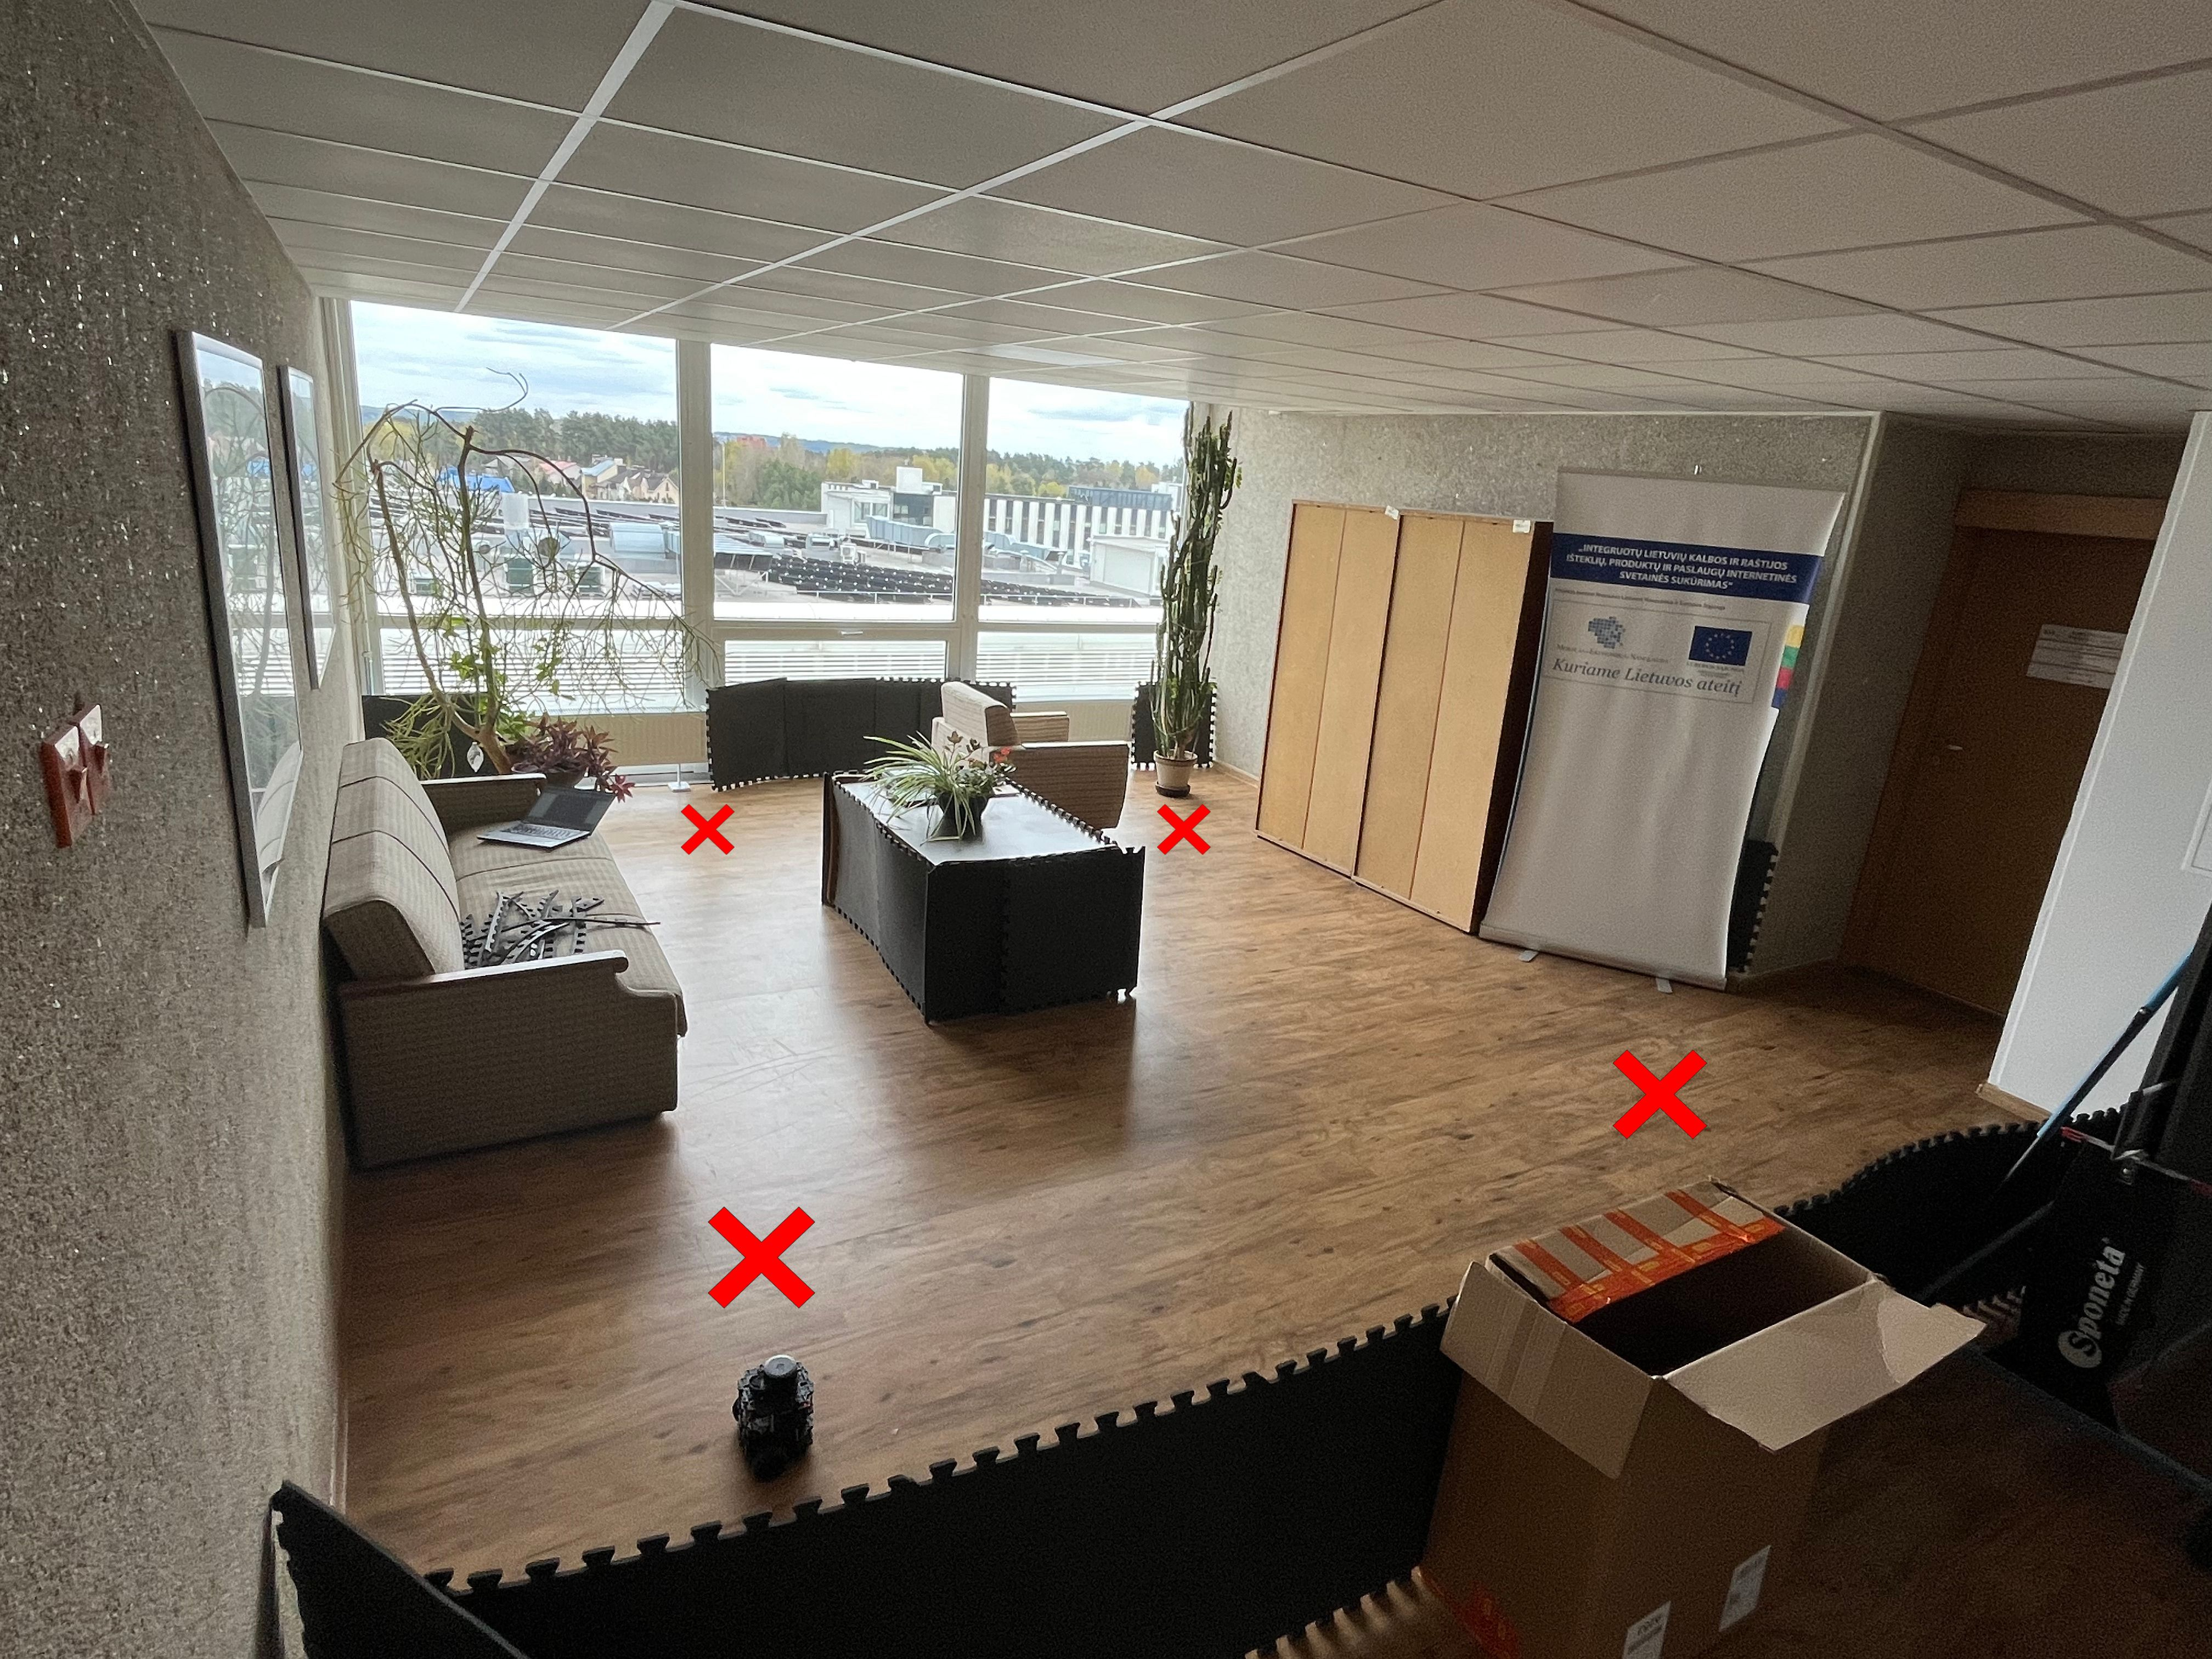
\includegraphics[width=\textwidth]{images/kamb1/1-w-marks.jpg}
\end{minipage}
\hfill
\begin{minipage}{0.32\textwidth}
  \centering
  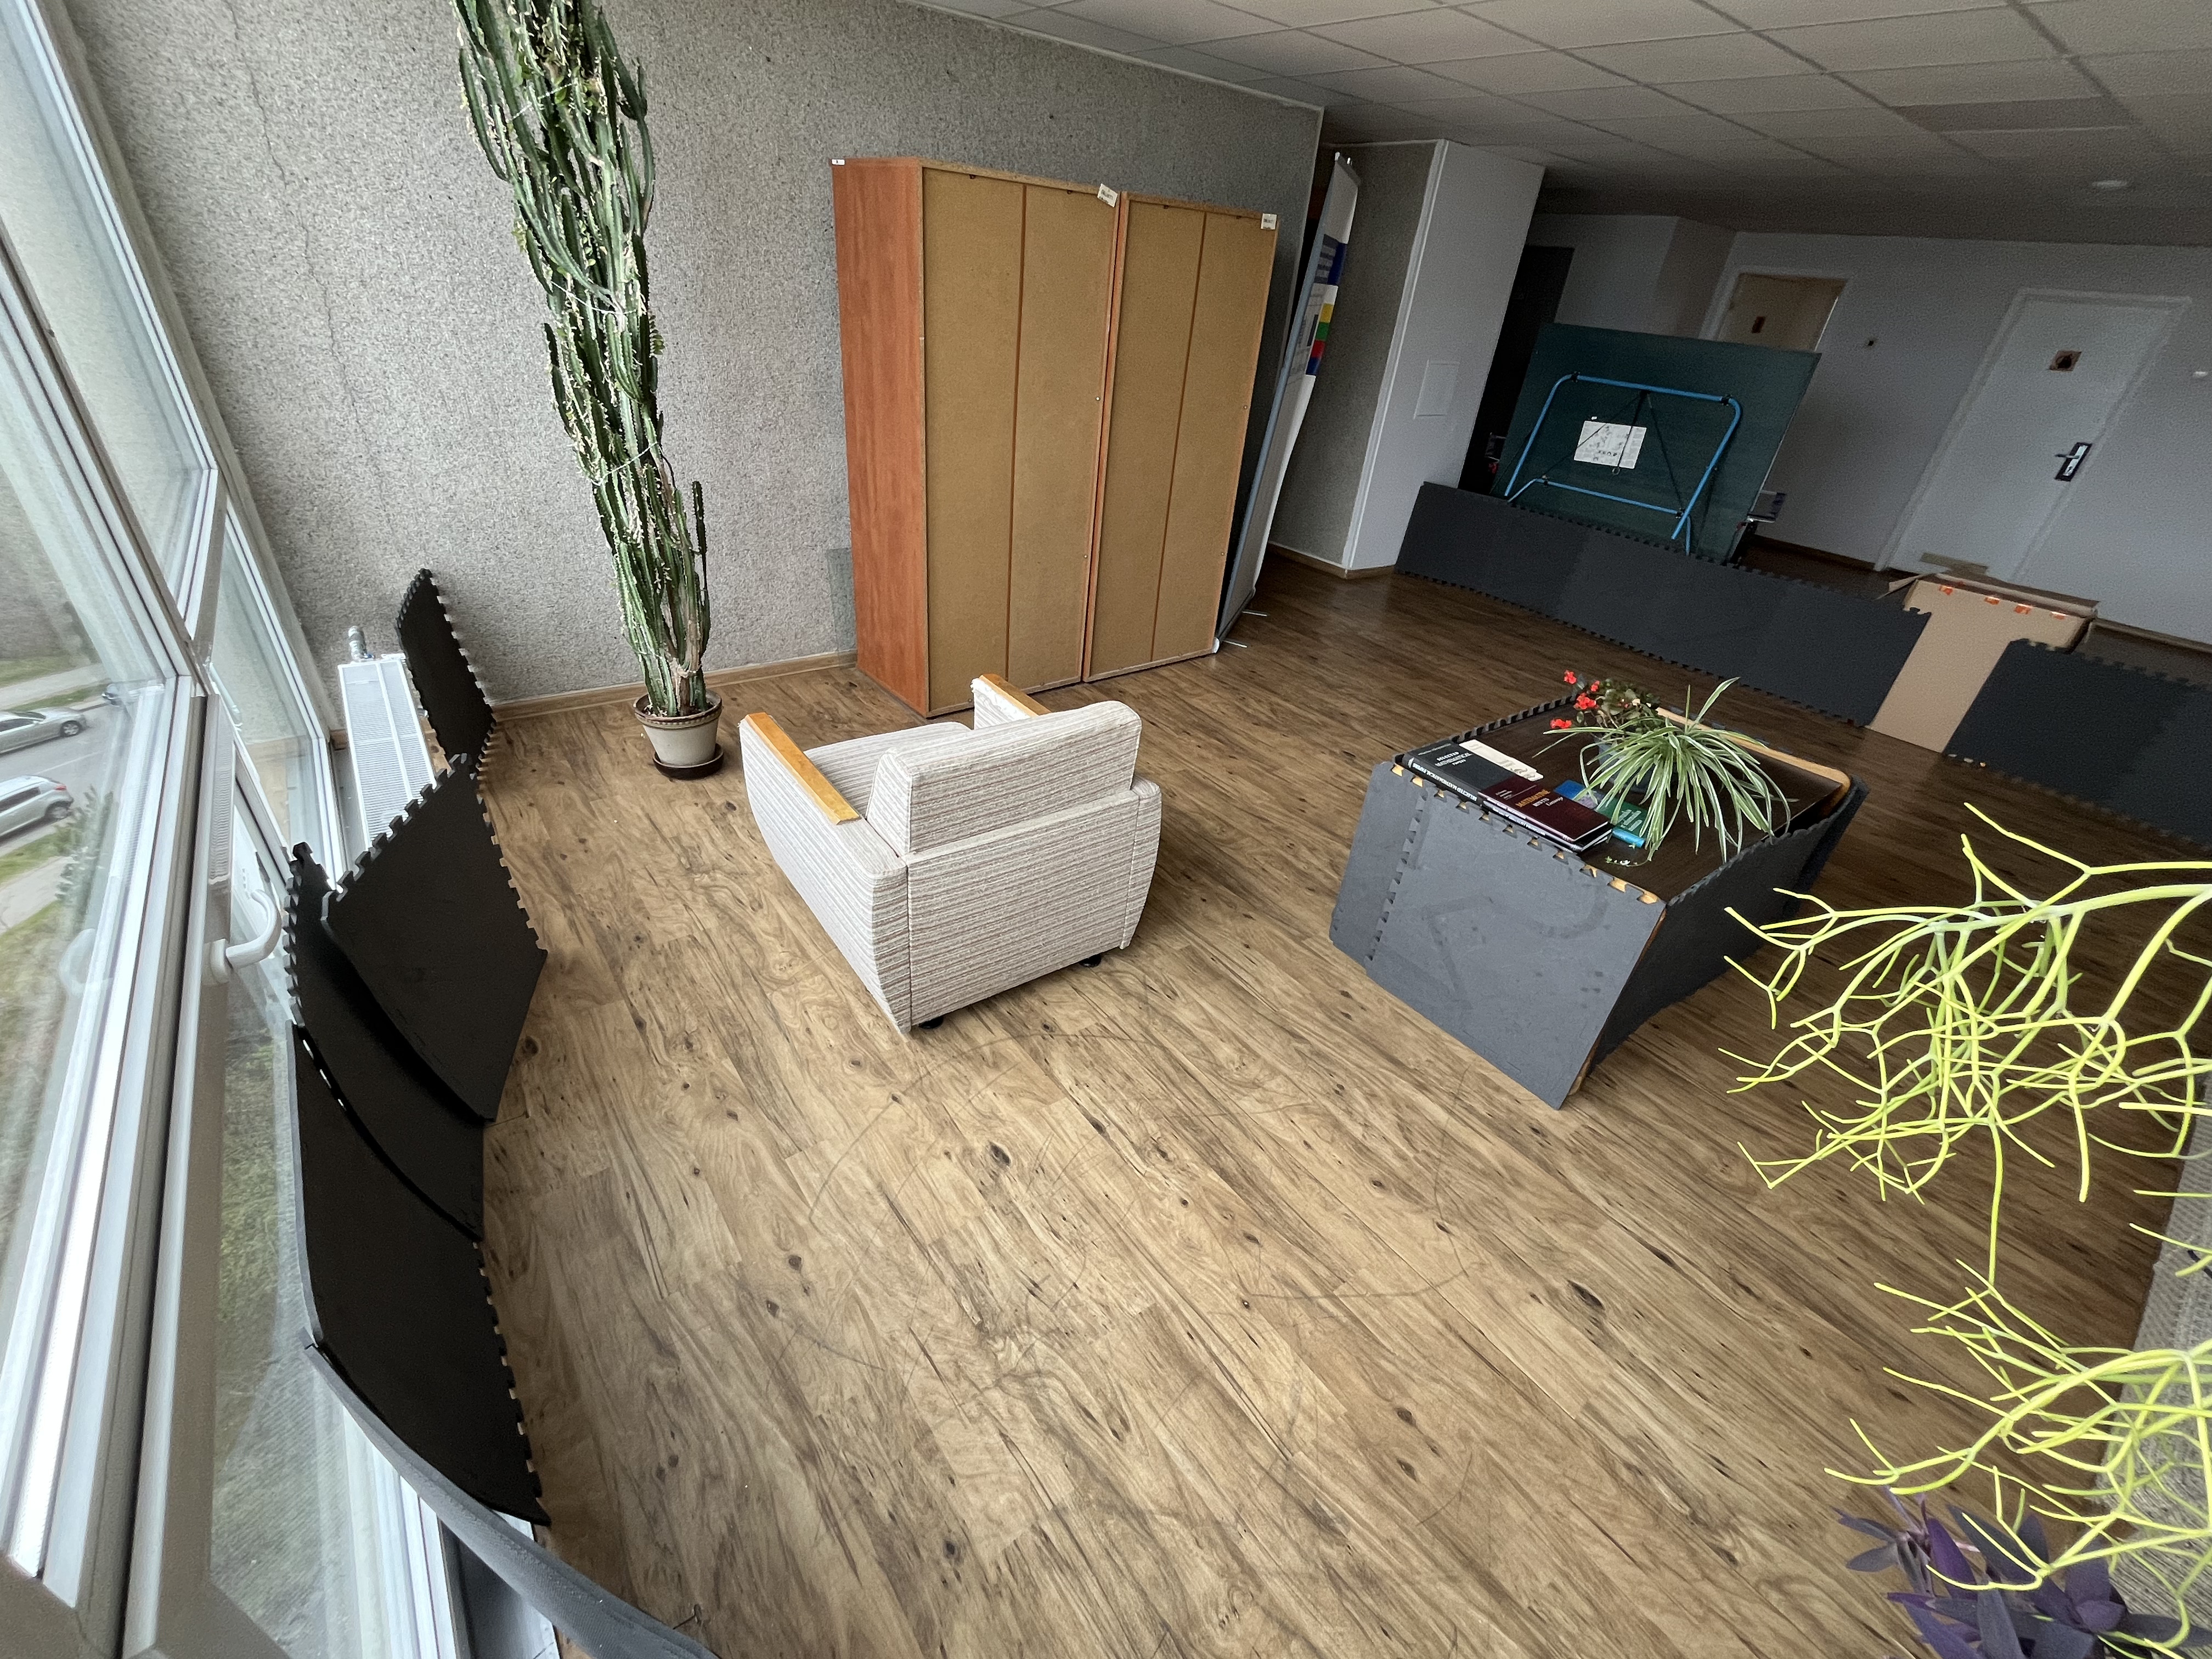
\includegraphics[width=\textwidth]{images/kamb1/2.jpg}
\end{minipage}
\hfill
\begin{minipage}{0.32\textwidth}
  \centering
  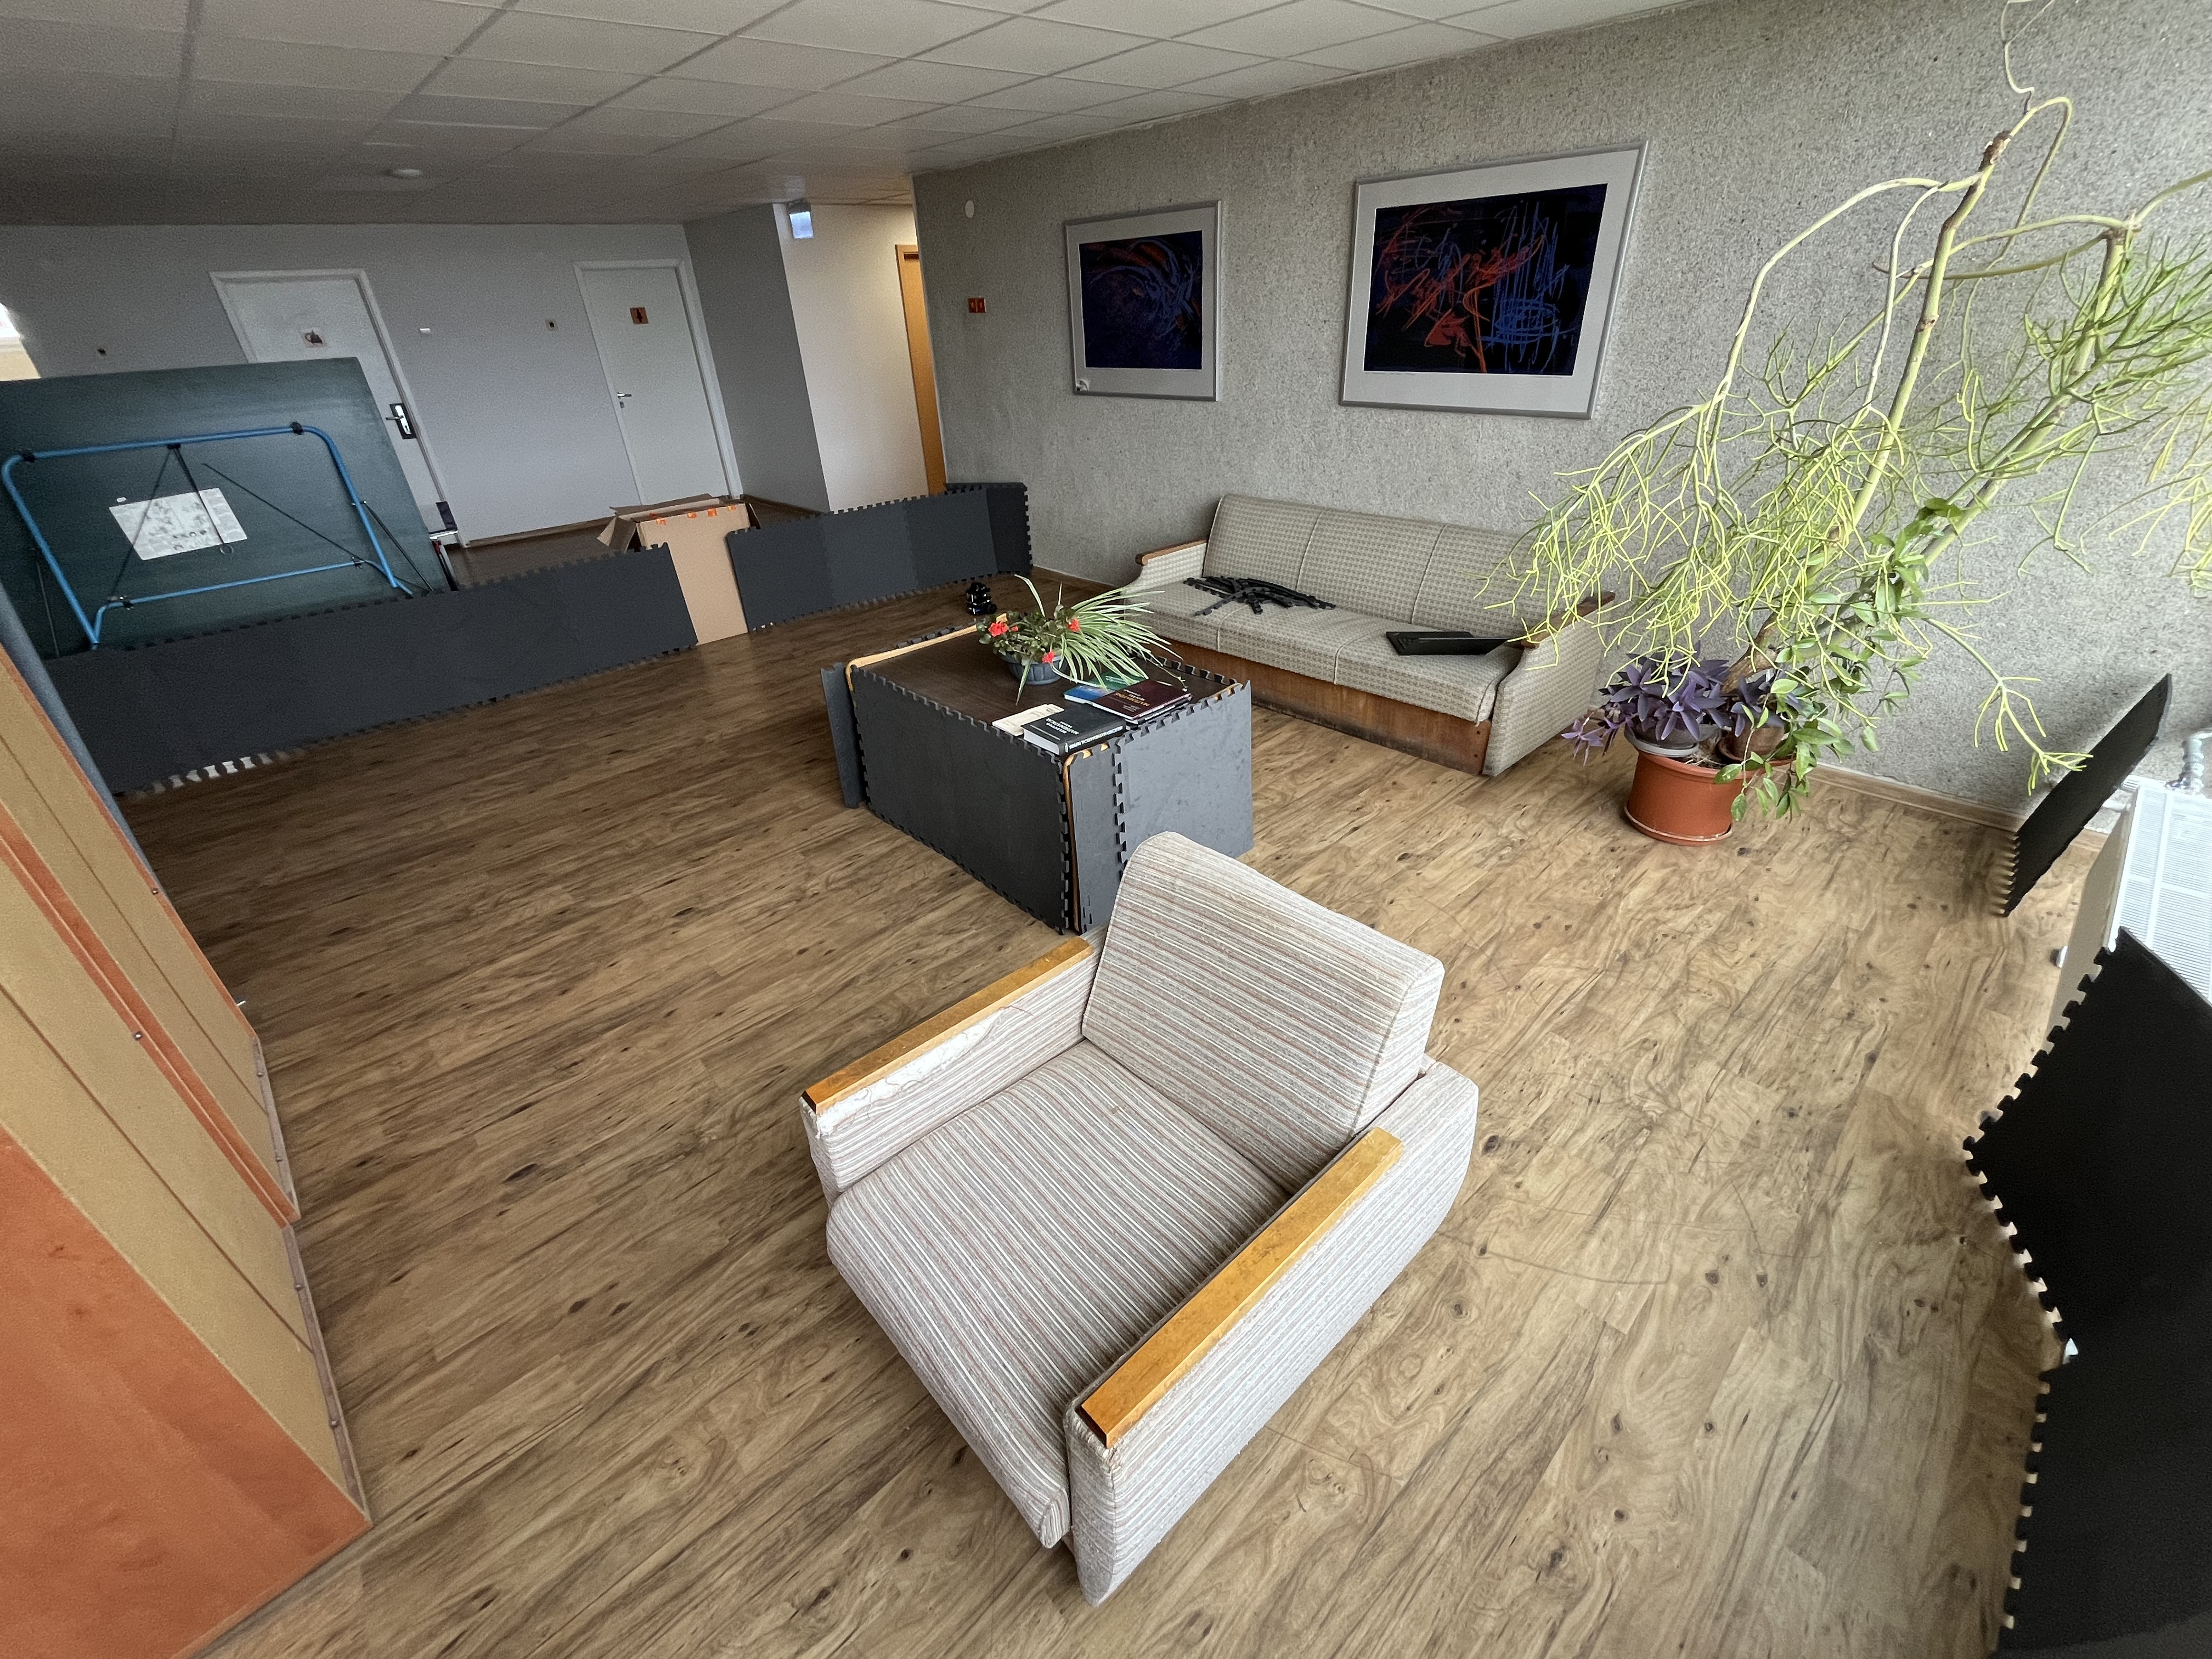
\includegraphics[width=\textwidth]{images/kamb1/3.jpg}
\end{minipage}
\caption{Pirmoji eksperimentinė aplinka. Raudonais X pažymėtos naudotos pradinės roboto pozicijos.}
\end{figure}

Šioje aplinkoje tikimasi, kad visi algoritmai turėtų gebėti pasiekti aukštą žemėlapio padengimą. Todėl svarbiausi palyginimo aspektai yra išžvalgymo laikas,
nuvažiuotas kelias ir galutinis padengimas. Jei algoritmas tokioje aplinkoje nuvažiuoja gerokai ilgesnį kelią arba užtrunka ilgiau pasiekdamas panašų
padengimą, tai rodo mažesnį tikslo parinkimo efektyvumą net santykinai paprastomis sąlygomis.

\subsubsection{Antroji aplinka: kambariai su siauru praėjimu}

Antroji aplinka sudaryta iš dviejų kambarių ir siauro koridoriaus praėjimo tarp jų. Didesniojo kambario apytikslūs matmenys yra 3,5~m $
\times$ 3,5~m, praėjimo - apie 0,5~m $\times$ 3~m, o kitos patalpos - apie 3~m $\times$ 2,5~m. Kambariuose taip pat yra objektų.

\begin{figure}[H]
\centering
\begin{minipage}{0.32\textwidth}
  \centering
  
\includegraphics[width=\textwidth]{images/kamb2/1-w-marks.jpg}
\end{minipage}
\hfill
\begin{minipage}{0.32\textwidth}
  \centering
  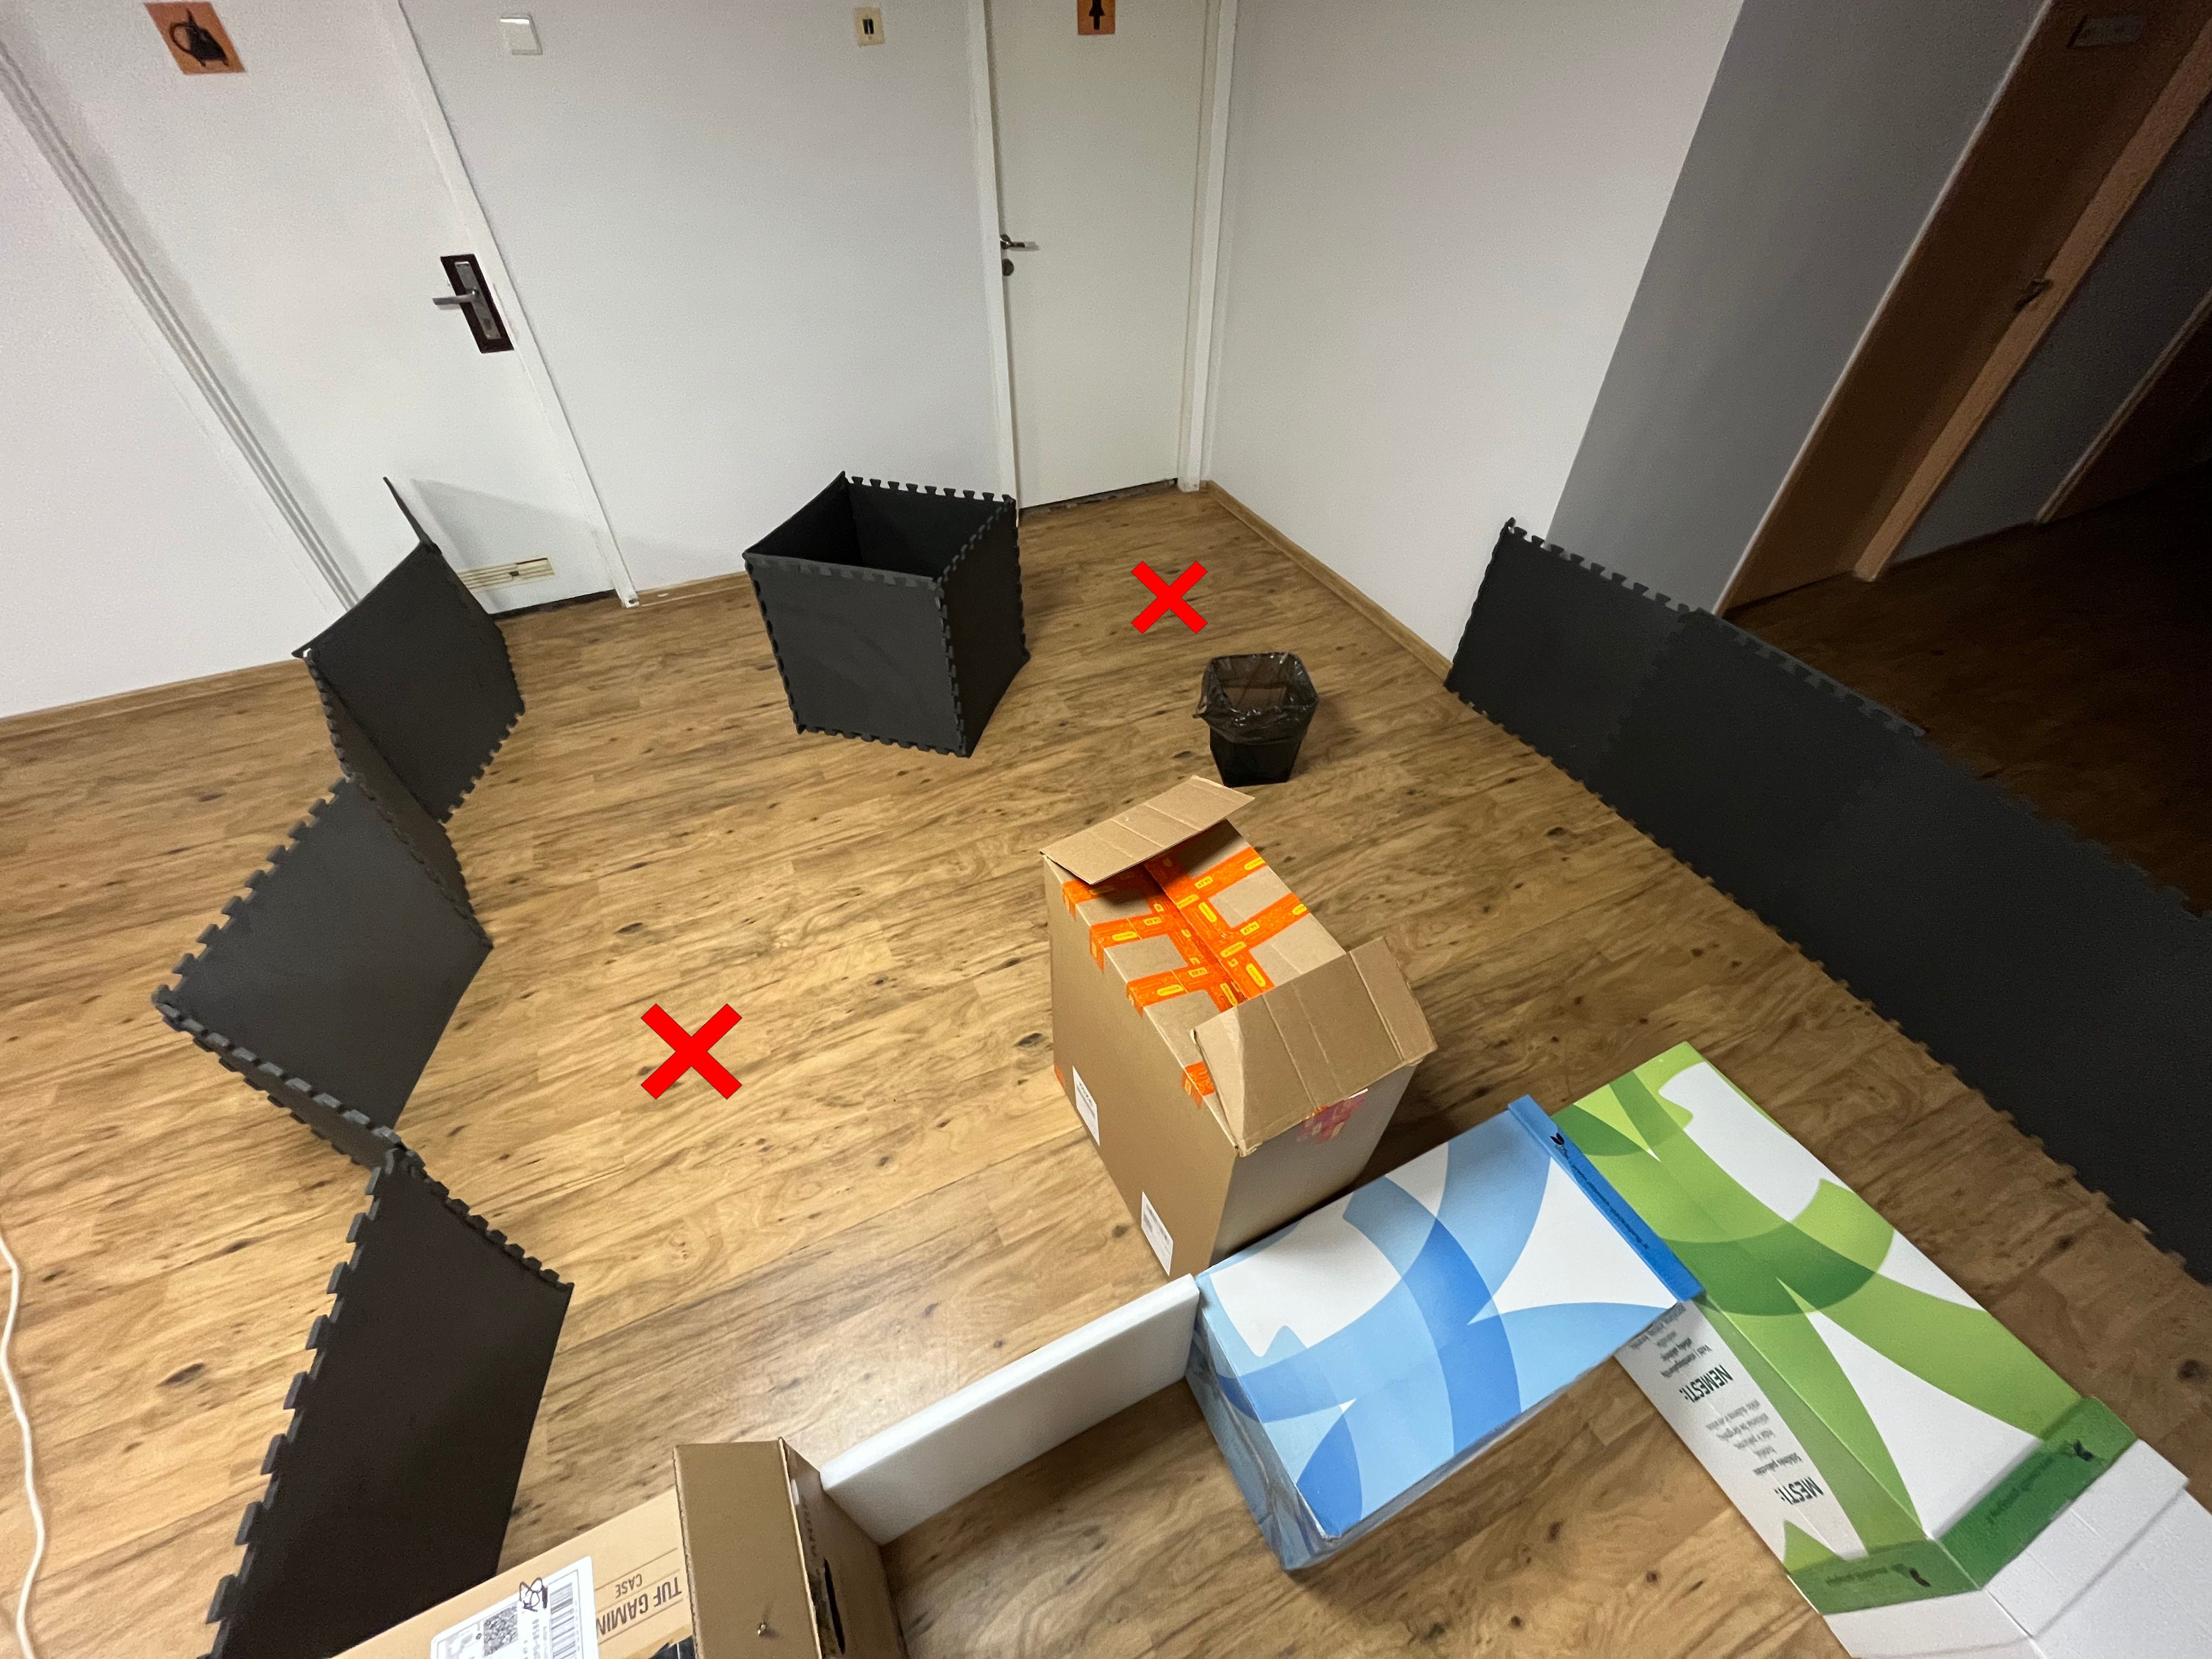
\includegraphics[width=\textwidth]{images/kamb2/2-w-marks.jpg}
\end{minipage}
\hfill
\begin{minipage}{0.32\textwidth}
  \centering
  
\includegraphics[width=\textwidth]{images/kamb2/3.jpg}
\end{minipage}
\caption{Antroji eksperimentinė aplinka. Raudonais X pažymėtos naudotos pradinės roboto pozicijos.}
\end{figure}

Ši aplinka parinkta todėl, kad siauri praėjimai yra svarbus realių vidaus patalpų iššūkis. Užimtumo tinkle siauras praėjimas gali būti pažymėtas netiksliai, o
navigacijos sistema gali sunkiau suplanuoti ir įvykdyti judėjimą iki tikslo. Tokia aplinka leidžia įvertinti, ar algoritmas geba aptikti ir pasiekti ribas,
esančias už siauro praėjimo, bei ar jis nepasirenka tikslų, kurie realiai yra sunkiai pasiekiami.

Šioje aplinkoje svarbu, ar algoritmas sugeba efektyviai išplėsti žemėlapį už siauro praėjimo ir ar dėl pasirinktos tikslų sekos robotas nepradeda daryti
perteklinio judėjimo pagrindinėje patalpoje. Todėl ši aplinka leidžia geriau atskleisti skirtumus tarp metodų, kurie renkasi artimiausias ribas, ir metodų,
kurie labiau įvertina informacijos kiekį arba aplinkos geometriją.

\subsubsection{Trečioji aplinka: ilgas koridorius su nišomis ir kliūtimis}

Trečioji aplinka yra ilgas koridorius, kurio ilgis yra 24~m, o plotis - apie 2,5~m. Koridoriuje yra dvi nišos ir kelios kliūtys. Ši aplinka
skiriasi nuo pirmųjų dviejų tuo, kad yra geometriškai ištęsta ir turi aiškią pagrindinę judėjimo kryptį.

\begin{figure}[H]
\centering
\begin{minipage}{0.48\textwidth}
  \centering
  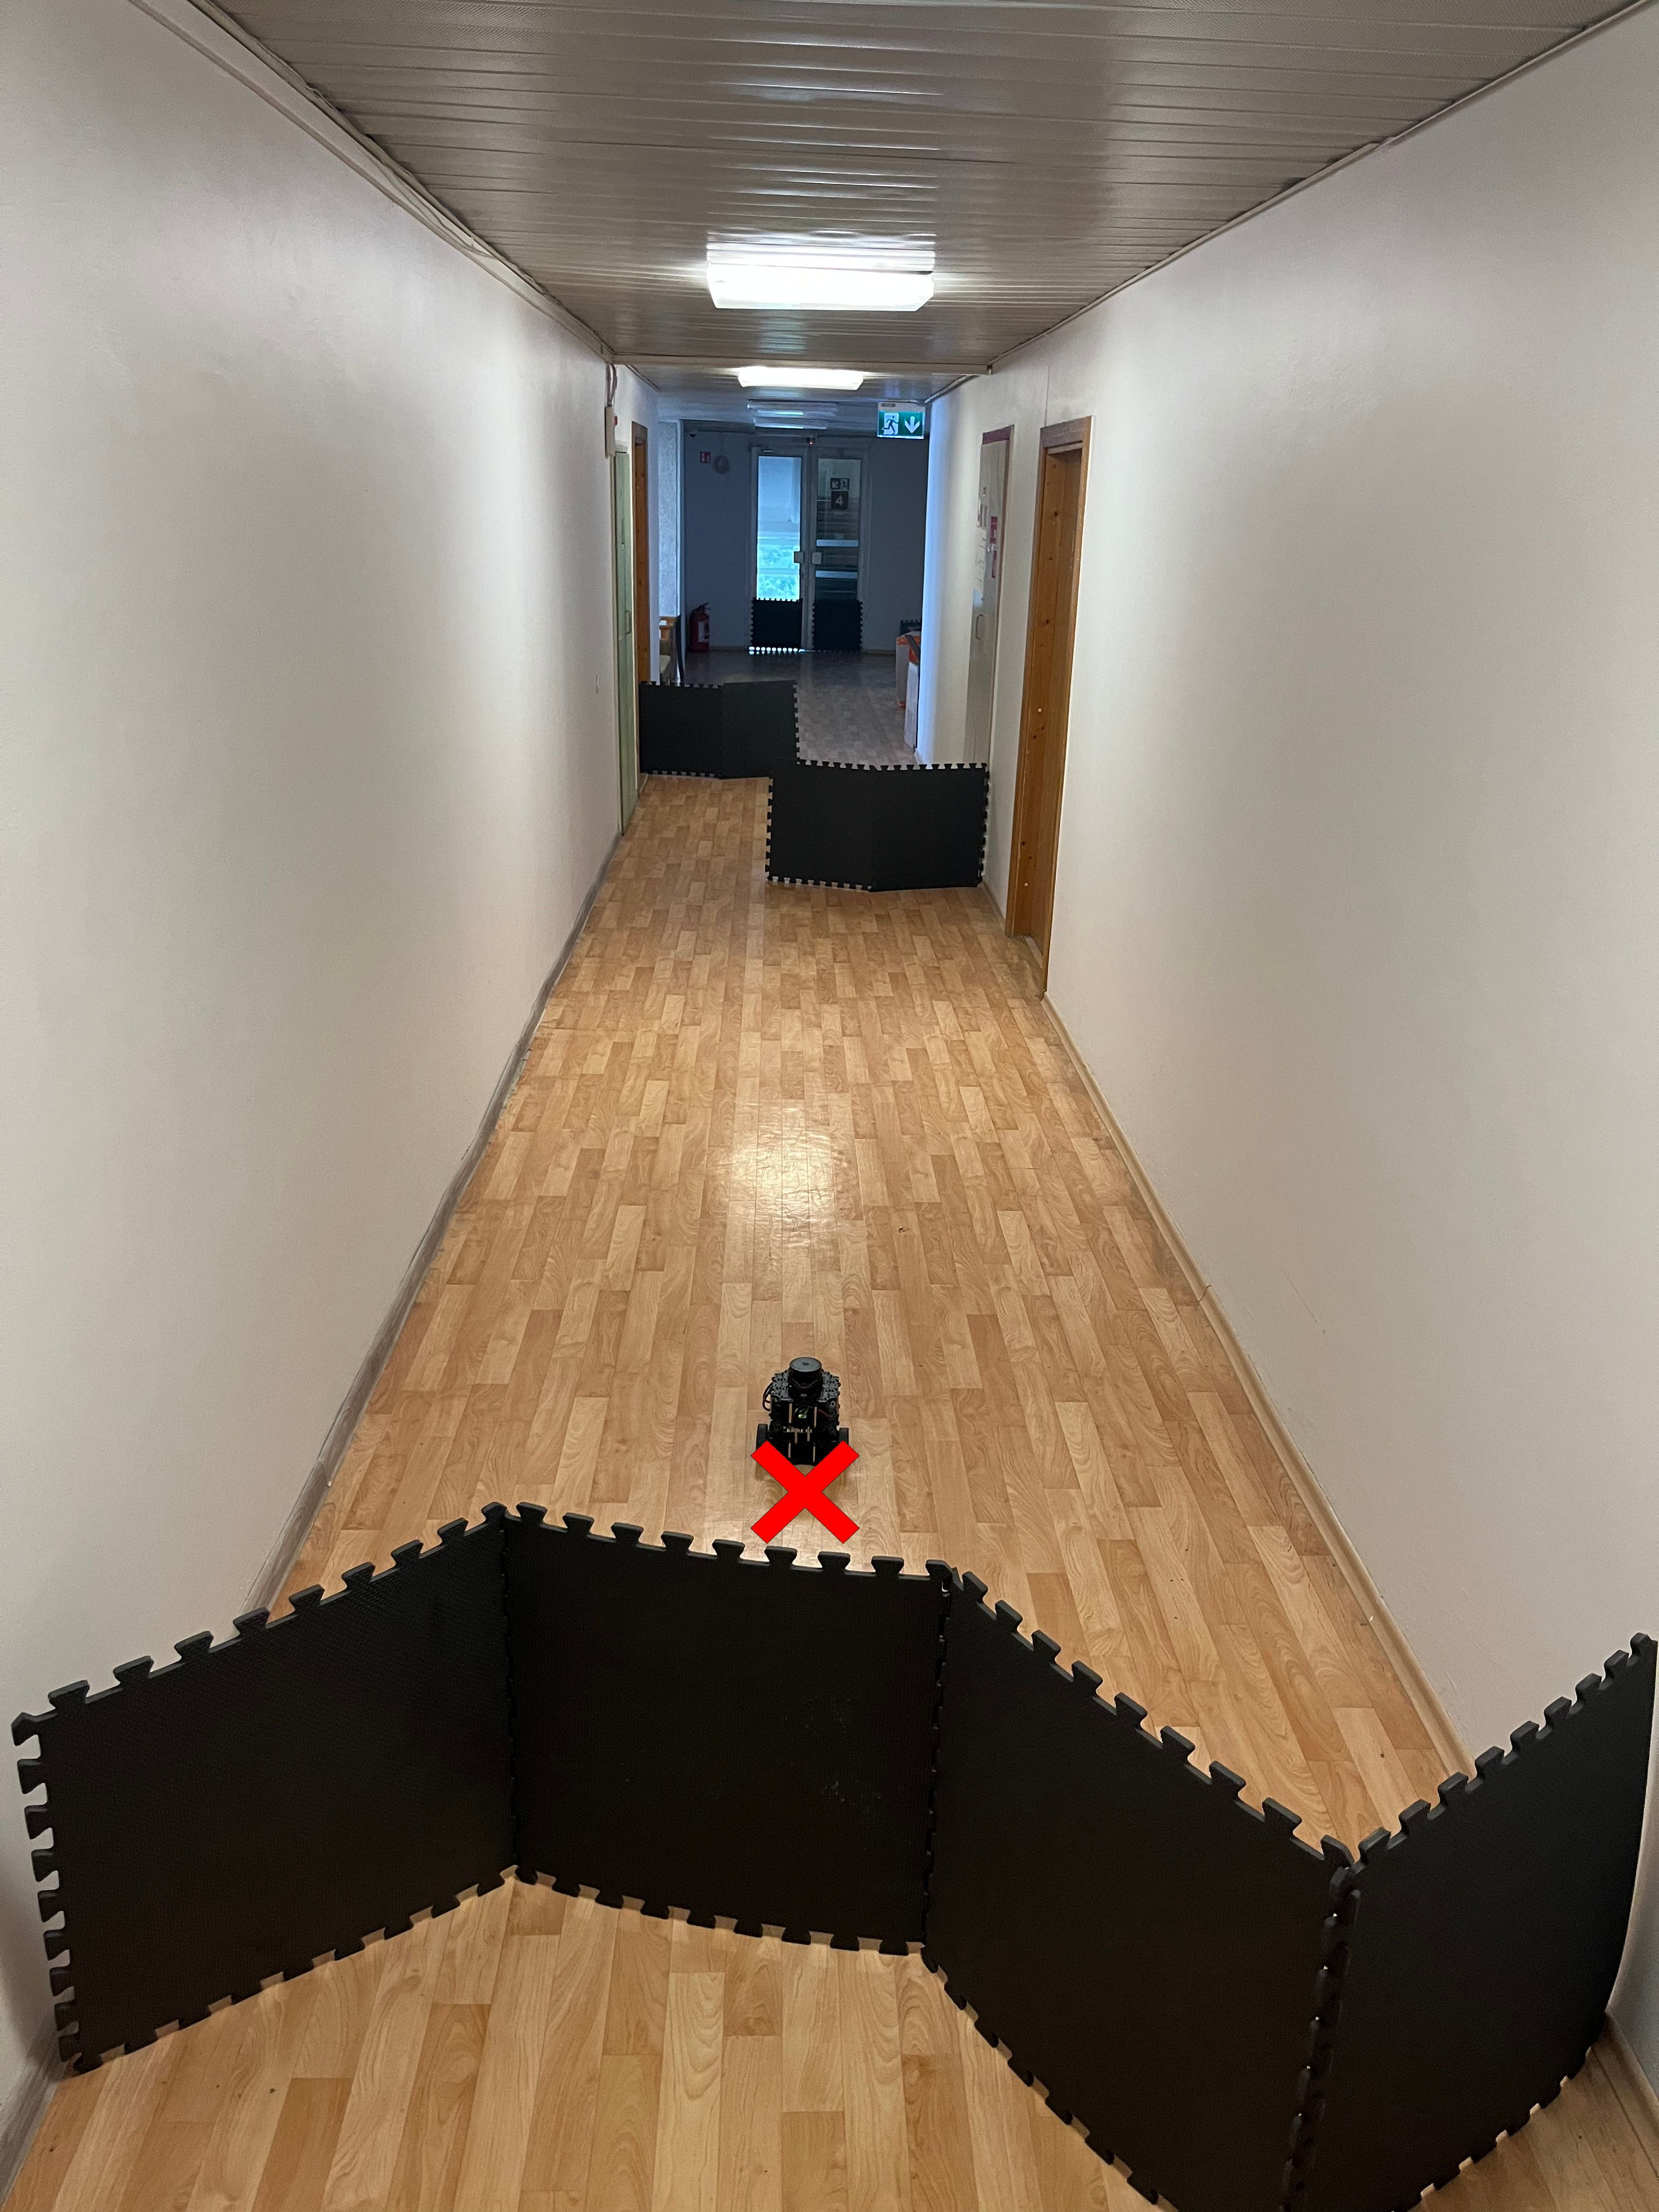
\includegraphics[width=\textwidth]{images/kamb3/1-w-mark.jpg}
\end{minipage}
\hfill
\begin{minipage}{0.48\textwidth}
  \centering
  
\includegraphics[width=\textwidth]{images/kamb3/2-w-marks.jpg}
\end{minipage}

\vspace{0.4em}

\begin{minipage}{0.48\textwidth}
  \centering
  
\includegraphics[width=\textwidth]{images/kamb3/3.jpg}
\end{minipage}
\hfill
\begin{minipage}{0.48\textwidth}
  \centering
  \includegraphics[width=\textwidth]{images/kamb3/4.jpg}
\end{minipage}
\caption{Trečioji eksperimentinė aplinka. Raudonais X pažymėtos naudotos pradinės roboto pozicijos.}
\end{figure}

Ilgas koridorius leidžia įvertinti, ar algoritmas geba nuosekliai plėsti žemėlapį išilgai aplinkos ir ar nesukuria perteklinio judėjimo tarp jau ištirtų
sričių. Šioje aplinkoje svarbus ne tik galutinis padengimas, bet ir kelio ilgis bei tikslo pasirinkimo nuoseklumas. Algoritmas, kuris dažnai renkasi
neinformatyvius arba mažus ribų fragmentus, gali sugeneruoti daugiau tikslų ir padidinti bendrą išžvalgymo laiką.

\subsection{Bandymų skaičius}

Pirmoje ir antroje aplinkose kiekvienas algoritmas vykdomas po keturis kartus. Šiose aplinkose naudotos keturios atsitiktinai parinktos kampinės pradinės
pozicijos, o kiekvienas algoritmas buvo paleistas iš tų pačių pažymėtų vietų. Trečioje aplinkoje kiekvienas algoritmas vykdomas po tris kartus, naudojant tris
atsitiktinai parinktas pradines pozicijas. Pakartotiniai bandymai reikalingi todėl, kad realaus roboto eksperimentuose rezultatai gali skirtis dėl jutiklių
matavimo pokyčių, lokalizacijos paklaidų, roboto pradinės orientacijos, nedidelių aplinkos pokyčių arba Nav2 planavimo sprendimų.

Vienkartinis bandymas nebūtų pakankamas algoritmų palyginimui, nes realioje sistemoje atsitiktiniai arba situaciniai veiksniai gali paveikti rezultatą. Keli
bandymai leidžia vertinti ne tik pavienį atvejį, bet ir bendresnę algoritmo elgseną toje pačioje aplinkoje.

\subsection{Bandymų eiga}

Kiekvienas bandymas atliekamas pagal tą pačią bendrą eigą:
\begin{enumerate}
  \item paruošiama eksperimentinė aplinka ir pašalinami pašaliniai trukdžiai;
  \item robotas pastatomas į pradinę poziciją;
  \item paleidžiamas \textit{bringup.launch.py} failas su pasirinktu išžvalgymo algoritmu; šis failas nuosekliai paleidžia roboto, SLAM, navigacijos ir išžvalgymo mazgus;
  \item robotas autonomiškai vykdo aplinkos išžvalgymą;
  \item pasibaigus bandymui užrašoma galutinė bandymo suvestinė;
  \item prieš kitą bandymą sistema paleidžiama iš naujo, kad bandymai būtų nepriklausomi.
\end{enumerate}

Kiekvieno bandymo metu operatorius nestabdo ir nekoreguoja roboto judėjimo. Algoritmo sprendimai priimami
automatiškai pagal tuo metu turimą užimtumo tinklą ir roboto poziciją.

\subsection{Eksperimentams svarbūs išžvalgymo mazgo parametrai}

Visi bandymai atliekami su ta pačia Nav2 ir \textit{slam\_toolbox} konfigūracija, kuri aprašyta 3 skyriuje. Atskirų algoritmų vidiniai parametrai pateikti 4
skyriuje. Šiame poskyryje pateikiami tik tie pagrindinio išžvalgymo mazgo parametrai, kurie tiesiogiai lemia bandymo eigą ir pabaigos sąlygą. Naudoti
parametrai pateikti \ref{tab:config-params} lentelėje.

\begin{table}[H]
\centering
\caption{Eksperimentams svarbūs išžvalgymo mazgo parametrai}
\label{tab:config-params}
\small
\setlength{\tabcolsep}{5pt}
\begin{tabular}{|l|l|p{0.55\textwidth}|}
\hline
\textbf{Parametras} & \textbf{Reikšmė} & \textbf{Paskirtis} \\
\hline
\textit{exploration\_loop\_rate} & 1 Hz & pagrindinio ciklo dažnis \\
\hline
\textit{goal\_timeout} & 60 s & maksimalus laikas vienam navigacijos tikslui pasiekti \\
\hline
\textit{failure\_cooldown} & 3 s & pauzė po nesėkmingo tikslo prieš skaičiuojant kitą \\
\hline
\textit{no\_goal\_strike\_limit} & 8 & eksperimento užbaigimo riba pagal iš eilės be tikslo grąžintų ciklų skaičių \\
\hline
\end{tabular}
\end{table}

Šie parametrai užtikrina, kad visų algoritmų bandymai būtų vykdomi pagal tą pačią ciklo, tikslo vykdymo ir pabaigos logiką. \textit{goal\_timeout}~=~60 s ir
\textit{failure\_cooldown}~=~3 s reiškia, kad nesėkmingas tikslas vienam bandymui gali kainuoti iki maždaug 63 s realaus laiko. Eksperimentas baigiamas tada,
kai algoritmas \textit{no\_goal\_strike\_limit}~=~8 kartus iš eilės negrąžina naujo tikslo.

\subsection{Palyginamumo užtikrinimas}

\textbf{Palyginamumas užtikrinamas} išlaikant tą pačią eksperimentinę aplinką, tą pačią programos konfigūraciją ir tas pačias pradines pozicijas kiekvienam algoritmui.
Skiriasi tik aktyvi išžvalgymo strategija, parenkama paleidimo metu.

Visiems algoritmams pateikiama \textbf{ta pati įvesties informacija}: užimtumo tinklas ir roboto pozicija. Visi tikslai siunčiami per tą pačią navigacijos veiksmų sąsają.
Tai leidžia sumažinti sisteminių skirtumų įtaką rezultatams.

Aplinkos objektų išdėstymas tarp bandymų nekeičiamas. Tokiu būdu siekiama, kad skirtumai tarp rezultatų būtų kuo labiau susiję su algoritmo elgsena, o ne su
aplinkos pokyčiais.

\subsection{Eksperimentų pabaigos sąlyga}

\textbf{Eksperimentas laikomas baigtu}, kai išžvalgymo strategija kelis ciklus iš eilės neberanda tinkamo naujo navigacijos tikslo. Pagal konfigūracijos lentelę
(\ref{tab:config-params}) naudojama \textit{no\_goal\_strike\_limit}~=~8 reikšmė, todėl išžvalgymas baigiamas tada, kai algoritmas aštuonis pagrindinio ciklo
kartus iš eilės grąžina rezultatą be naujo tikslo. Kadangi pagrindinis ciklas vykdomas 1~Hz dažniu, tai atitinka maždaug 8~s laikotarpį be naujo tinkamo
tikslo. Tai reiškia, kad kiekvienas algoritmas pats nusprendžia, kada išžvalgymas užbaigiamas, todėl rezultatai atspindi ne tik judėjimo trukmę, bet ir
algoritmo gebėjimą rasti naujus tikslus tol, kol aplinka dar nėra pilnai išžvalgyta.

Toliau pateikiami penkių aplinkos išžvalgymo algoritmų eksperimentų rezultatai trijose realiose vidaus aplinkose. Kiekvienai aplinkai pateikiami keli rezultatų pjūviai: bandymų vidurkiai, rezultatų intervalai ir
standartinis nuokrypis. Vidurkiai parodo tipinę algoritmo elgseną, intervalai leidžia matyti
mažiausias ir didžiausias bandymuose užfiksuotas reikšmes, o standartinis nuokrypis naudojamas
išžvalgymo laiko ir nuvažiuoto kelio stabilumui įvertinti.
Stulpelis „Tikslai“ nurodo, kiek navigacijos tikslų išžvalgymo algoritmas išsiuntė Nav2 sistemai. Stulpeliai „Pasiekta“ ir „Nepavyko“ parodo, kiek iš šių
tikslų buvo sėkmingai pasiekta arba nepasiekta. Vidurkių lentelėse pateikiamas vidutinis tikslų skaičius vienam bandymui.

\subsection{Pirmosios aplinkos rezultatai}

Pirmoji aplinka buvo paprastas kambarys su keliais objektais. Šioje aplinkoje visi algoritmai pasiekė panašų žemėlapio padengimą, kuris pagal turimus bandymus
buvo apie 95-97~\%. Vienas iš šioje aplinkoje sudarytų žemėlapių pateiktas \ref{fig:map-room1} pav.

\begin{figure}[H]
\centering
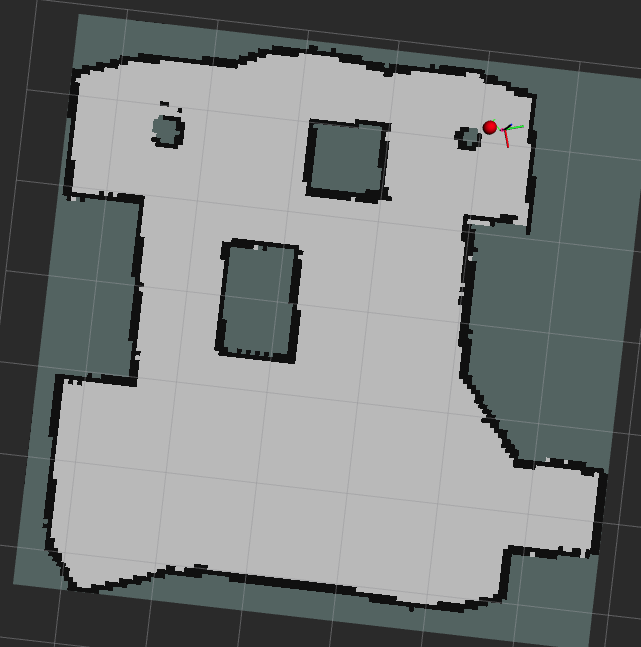
\includegraphics[width=0.72\textwidth]{images/sudarytas_zemelap/1_kamb.png}
\caption{Pirmojoje aplinkoje sudaryto žemėlapio pavyzdys}
\label{fig:map-room1}
\end{figure}

Pirmosios aplinkos rezultatų vidurkiai pateikti \ref{tab:results-room1-avg} lentelėje.

\begin{table}[H]
\centering
\caption{Pirmosios aplinkos rezultatų vidurkiai}
\label{tab:results-room1-avg}
\small
\setlength{\tabcolsep}{3pt}
\begin{tabular}{|l|c|c|c|c|c|c|c|}
\hline
\textbf{Algoritmas} & \textbf{$n$} & \textbf{Laikas, s} & \textbf{Padeng., \%} & \textbf{Kelias, m} & \textbf{Tikslai} & \textbf{Pasiekta} & \textbf{Nepavyko} \\
\hline
BFS & 4 & 244,4 & \textbf{96,6} & 17,26 & 11,5 & 10,5 & 1,0 \\
\hline
Artimiausia riba & 4 & 207,9 & 95,2 & \textbf{14,77} & 9,0 & 8,0 & 1,0 \\
\hline
Informacijos prieaugis & 4 & 242,2 & 95,3 & 18,01 & 8,8 & 6,8 & 2,5 \\
\hline
RRT & 4 & 202,2 & 95,0 & 16,43 & 7,5 & 6,8 & 0,8 \\
\hline
Voronoi & 4 & \textbf{200,9} & 95,2 & 17,40 & 6,8 & 6,5 & \textbf{0,5} \\
\hline
\end{tabular}
\end{table}

\textbf{Pagal vidutines reikšmes} mažiausią išžvalgymo laiką turėjo Voronoi ir RRT algoritmai (atitinkamai 200,9~s ir 202,2~s). Didžiausias vidutinis padengimas
užfiksuotas BFS algoritmui (96,6~\%), nors visi kiti algoritmai išliko 95~\% slenksčio ribose. Trumpiausias vidutinis kelias - 14,77~m - užfiksuotas
artimiausios ribos algoritmui, kuris pagal idėją renkasi mažiausiu atstumu pasiekiamą ribą. Informacijos prieaugio algoritmas turėjo didžiausią
vidutinį nepasiektų tikslų skaičių (2,5), o BFS - didžiausią vidutinį išsiųstų tikslų skaičių (11,5), kuris atspindi šio algoritmo polinkį rinktis pirmą
tinkamą ribą be papildomo kandidatų vertinimo.

Bandymų rezultatų intervalai pateikti \ref{tab:results-room1-disp} lentelėje.

\begin{table}[H]
\centering
\caption{Pirmosios aplinkos rezultatų intervalai}
\label{tab:results-room1-disp}
\small
\setlength{\tabcolsep}{3pt}
\begin{tabular}{|l|c|c|c|c|c|c|}
\hline
\textbf{Algoritmas} & \textbf{$n$} & \textbf{Laikas, s} & \textbf{Padeng., \%} & \textbf{Kelias, m} & \textbf{Nepavyko} \\
\hline
BFS & 4 & 165,8--315,7 & 95,2--99,8 & 13,24--21,10 & 0--3 \\
\hline
Artimiausia riba & 4 & 137,2--263,2 & 95,0--95,5 & 11,10--17,45 & 0--3 \\
\hline
Informacijos prieaugis & 4 & 215,2--291,1 & 95,2--95,6 & 15,19--22,09 & 0--4 \\
\hline
RRT & 4 & 134,4--245,4 & 94,5--95,6 & 11,72--25,15 & 0--2 \\
\hline
Voronoi & 4 & 163,4--238,4 & 95,2--95,4 & 12,74--19,45 & 0--2 \\
\hline
\end{tabular}
\end{table}

Intervalų lentelė rodo, kad vidurkis šioje aplinkoje paslepia didelius skirtumus tarp atskirų bandymų. BFS algoritmo bandymų laikas svyravo nuo 165,8~s iki
315,7~s, t. y. ilgiausias bandymas truko beveik dvigubai ilgiau už trumpiausią. Šį skirtumą paaiškina nepasiektų tikslų skaičius - ilgiausiame BFS bandyme
užfiksuoti 3 nepasiekti tikslai, o trumpiausiame - nė vieno. Panaši situacija matoma artimiausios ribos algoritme, kurio paskutinis bandymas grąžino 3
nepasiektus tikslus, nors kiti bandymai turėjo ženkliai mažiau nesėkmingų tikslų. Informacijos prieaugio algoritmui būdingas plačiausias nepasiektų tikslų intervalas (0--4): trys iš
keturių bandymų grąžino nuo dviejų iki keturių nesėkmių, todėl vidutinis laikas išauga, nors trumpiausias bandymas buvo gana panašus į kitų algoritmų. RRT
algoritmo kelio intervalas (11,72--25,15~m) yra plačiausias tarp visų algoritmų; tai paaiškina stochastinis medžio augimas, kuris gali grąžinti tolimas šakas
net mažoje aplinkoje.  Pirmojoje aplinkoje Voronoi algoritmo kelio ir laiko intervalai buvo siauriausi. Tokį rezultatą galėjo lemti paprastesnė patalpos geometrija: joje sudaroma Voronoi struktūra tarp bandymų
mažai keitėsi, todėl ir parenkami tikslai buvo panašesni.

\subsection{Antrosios aplinkos rezultatai}

Antroji aplinka buvo sudėtingesnė: ją sudarė pirmasis kambarys, siauras tunelio tipo praėjimas ir antroji patalpa. Šioje aplinkoje visi algoritmai
pasiekė panašų galutinį padengimą, apie 98~\%. Vienas iš šioje aplinkoje sudarytų žemėlapių pateiktas \ref{fig:map-room2} pav.

\begin{figure}[H]
\centering
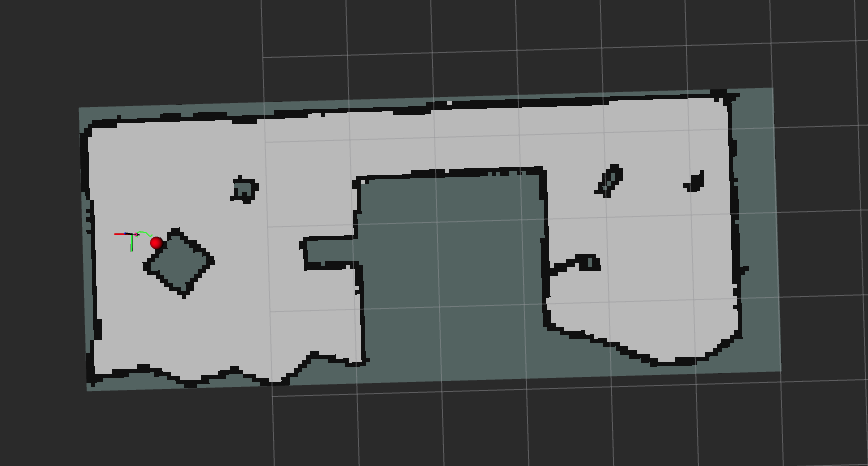
\includegraphics[width=0.72\textwidth]{images/sudarytas_zemelap/2_kamb.png}
\caption{Antrojoje aplinkoje sudaryto žemėlapio pavyzdys}
\label{fig:map-room2}
\end{figure}

Antrosios aplinkos rezultatų vidurkiai pateikti \ref{tab:results-room2-avg} lentelėje.

\begin{table}[H]
\centering
\caption{Antrosios aplinkos rezultatų vidurkiai}
\label{tab:results-room2-avg}
\small
\setlength{\tabcolsep}{3pt}
\begin{tabular}{|l|c|c|c|c|c|c|c|}
\hline
\textbf{Algoritmas} & \textbf{$n$} & \textbf{Laikas, s} & \textbf{Padeng., \%} & \textbf{Kelias, m} & \textbf{Tikslai} & \textbf{Pasiekta} & \textbf{Nepavyko} \\
\hline
BFS & 4 & 358,7 & 98,4 & 20,02 & 19,3 & 16,7 & 3,0 \\
\hline
Artimiausia riba & 4 & \textbf{162,1} & 98,4 & 13,79 & 11,0 & 11,0 & \textbf{0,0} \\
\hline
Informacijos prieaugis & 4 & 172,8 & 98,4 & \textbf{13,56} & 10,7 & 10,7 & \textbf{0,0} \\
\hline
RRT & 4 & 203,4 & 98,3 & 17,62 & 9,3 & 8,7 & 1,0 \\
\hline
Voronoi & 4 & 224,7 & \textbf{98,5} & 18,67 & 10,3 & 9,7 & 1,0 \\
\hline
\end{tabular}
\end{table}

\textbf{Pagal vidurkius antrojoje aplinkoje} pirmavo artimiausios ribos algoritmas, kurio vidutinė trukmė buvo 162,1~s. Informacijos prieaugio algoritmas turėjo
trumpiausią vidutinį kelią - 13,56~m - ir vidutinį laiką (172,8~s), tik šiek tiek didesnį už artimiausios ribos rezultatą. Didžiausias vidutinis padengimas
užfiksuotas Voronoi algoritmui (98,5~\%), nors skirtumas nuo kitų algoritmų buvo nedidelis. BFS algoritmas šioje aplinkoje turėjo didžiausią vidutinį laiką (358,7 s) ir didžiausią vidutinį nepasiektų tikslų skaičių (3,0).

Bandymų rezultatų intervalai pateikti \ref{tab:results-room2-disp} lentelėje.

\begin{table}[H]
\centering
\caption{Antrosios aplinkos rezultatų intervalai}
\label{tab:results-room2-disp}
\small
\setlength{\tabcolsep}{3pt}
\begin{tabular}{|l|c|c|c|c|c|}
\hline
\textbf{Algoritmas} & \textbf{$n$} & \textbf{Laikas, s} & \textbf{Padeng., \%} & \textbf{Kelias, m} & \textbf{Nepavyko} \\
\hline
BFS & 4 & 179,8--492,7 & 97,6--98,8 & 10,99--29,35 & 0--6 \\
\hline
Artimiausia riba & 4 & 146,1--181,1 & 98,4--98,4 & 11,35--17,15 & 0--0 \\
\hline
Informacijos prieaugis & 4 & 138,1--218,1 & 98,0--98,6 & 11,90--16,48 & 0--0 \\
\hline
RRT & 4 & 140,4--245,3 & 97,8--98,6 & 11,34--25,00 & 0--2 \\
\hline
Voronoi & 4 & 183,4--280,3 & 98,4--98,6 & 16,66--21,55 & 0--4 \\
\hline
\end{tabular}
\end{table}

Antrojoje aplinkoje rezultatų intervalų skirtumas itin ryškiai matomas BFS algoritme: trumpiausias bandymas truko 179,8~s be nepasiektų tikslų, o ilgiausias - 492,7~s
su trimis nepasiektais tikslais ir 29,35~m keliu. Nesėkmingi tikslai grupavosi trijuose iš keturių bandymų, jų skaičius svyravo nuo 3 iki 6, tik pirmajame bandyme nesėkmių nebuvo, o tai lemia didelę laiko sklaidą. Tuo tarpu artimiausios ribos ir informacijos prieaugio algoritmai išlaikė nulinį
nepasiektų tikslų skaičių visuose bandymuose, todėl jų laiko intervalai (atitinkamai 146,1--181,1~s ir 138,1--218,1~s) yra reikšmingai siauresni. Voronoi algoritmas trečiajame bandyme užfiksavo keturis nepasiektus tikslus, kituose trijuose bandymuose nesėkmių nebuvo. RRT kelio intervalas 11,34--25,00~m vėl iliustruoja stochastiškumo įtaką: net toje pačioje
aplinkoje robotas gali nukeliauti dvigubai didesnį atstumą priklausomai nuo medžio augimo eigos.

RRT algoritmo elgsena antrojoje aplinkoje papildomai iliustruota \ref{fig:rrt-room2-goals} pav. Paveiksle matyti, kad robotui esant pirmojoje patalpoje dalis
netoliese esančios nežinomos srities dar nėra atskleista, tačiau sugeneruotas tikslas nukreipiamas į kitą patalpą. Raudonas taškas paveiksle žymi tuo metu
sugeneruotą navigacijos tikslą. Vėliau robotui jau esant
antrojoje patalpoje, naujas tikslas vėl sugeneruojamas pirmojoje patalpoje. Tokia tikslų seka padidina grįžimų tarp patalpų skaičių ir gali paaiškinti
didesnę RRT kelio bei laiko sklaidą antrojoje aplinkoje.

\begin{figure}[H]
\centering
\begin{minipage}{0.48\textwidth}
\centering
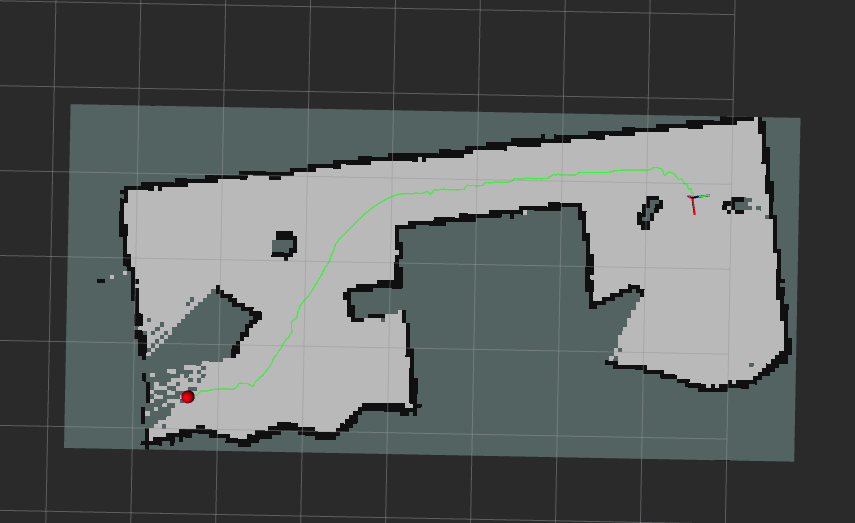
\includegraphics[width=\textwidth]{images/BFS-2kamb/tolimas-kelias-i-1.png}
\end{minipage}
\hfill
\begin{minipage}{0.48\textwidth}
\centering
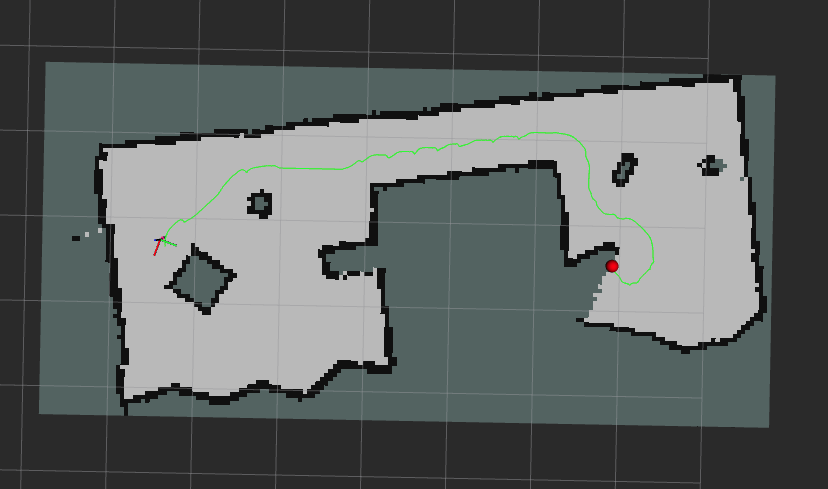
\includegraphics[width=\textwidth]{images/BFS-2kamb/tolimas-kelias-i-2.png}
\end{minipage}
\caption{RRT algoritmo tikslų generavimo pavyzdys antrojoje aplinkoje}
\label{fig:rrt-room2-goals}
\end{figure}

Šis pavyzdys rodo, kad RRT strategija dėl imtimi pagrįsto medžio plėtimo ne visada išlaiko lokaliai nuoseklų išžvalgymą. Antrojoje aplinkoje tai gali lemti
papildomus judėjimus tarp patalpų ir didesnį bandymų trukmės skirtumą.

\subsection{Trečiosios aplinkos rezultatai}

Trečioji aplinka buvo ilgas koridorius su nišomis ir kliūtimis. Šioje aplinkoje beveik visi algoritmai pasiekė 99,7-100~\% padengimą, tačiau veikimo laikas
ir nuvažiuotas kelias skyrėsi reikšmingai. Vienas iš šioje aplinkoje sudarytų žemėlapių pateiktas \ref{fig:map-room3} pav.

\begin{figure}[H]
\centering
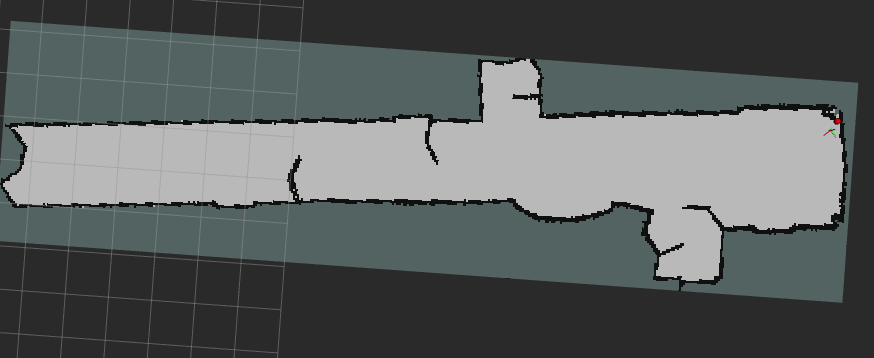
\includegraphics[width=0.72\textwidth]{images/sudarytas_zemelap/3_kamb.png}
\caption{Trečiojoje aplinkoje sudaryto žemėlapio pavyzdys}
\label{fig:map-room3}
\end{figure}

Trečiosios aplinkos rezultatų vidurkiai pateikti \ref{tab:results-room3-avg} lentelėje.

\begin{table}[H]
\centering
\caption{Trečiosios aplinkos rezultatų vidurkiai}
\label{tab:results-room3-avg}
\small
\setlength{\tabcolsep}{3pt}
\begin{tabular}{|l|c|c|c|c|c|c|c|}
\hline
\textbf{Algoritmas} & \textbf{$n$} & \textbf{Laikas, s} & \textbf{Padeng., \%} & \textbf{Kelias, m} & \textbf{Tikslai} & \textbf{Pasiekta} & \textbf{Nepavyko} \\
\hline
BFS & 3 & 533,6 & \textbf{100,0} & 37,74 & 40,0 & 38,7 & 1,7 \\
\hline
Artimiausia riba & 3 & 342,9 & 99,9 & 31,69 & 19,7 & 17,3 & 3,0 \\
\hline
Informacijos prieaugis & 3 & \textbf{259,1} & \textbf{100,0} & \textbf{27,28} & 12,0 & 11,7 & \textbf{0,3} \\
\hline
RRT & 3 & 418,7 & 99,7 & 38,42 & 21,3 & 18,0 & 4,0 \\
\hline
Voronoi & 3 & 567,9 & \textbf{100,0} & 54,50 & 23,0 & 20,0 & 5,7 \\
\hline
\end{tabular}
\end{table}

\textbf{Pagal vidurkius trečiojoje aplinkoje} mažiausią laiką ir trumpiausią kelią turėjo informacijos prieaugio algoritmas (259,1~s ir 27,28~m). Šis rezultatas
atitinka teorinę algoritmo savybę: ilgesnėje aplinkoje, kurioje vienas kandidatas gali atskleisti daug naujos informacijos, prieaugio vertinimas dažnai
parenka tolesnes, bet vertingesnes ribas, o ne artimiausias. BFS, informacijos prieaugio ir Voronoi algoritmai pasiekė 100~\% vidutinį padengimą. Voronoi
algoritmui šioje aplinkoje teko didžiausias vidutinis kelias (54,50~m) ir didžiausias vidutinis nepasiektų tikslų skaičius (5,7), o BFS rodė didžiausią
vidutinį išsiųstų tikslų skaičių (40,0) - ilgame koridoriuje šis algoritmas sukuria daug smulkių tikslų, esančių arti vienas kito.

Bandymų rezultatų intervalai pateikti \ref{tab:results-room3-disp} lentelėje.

\begin{table}[H]
\centering
\caption{Trečiosios aplinkos rezultatų intervalai}
\label{tab:results-room3-disp}
\small
\setlength{\tabcolsep}{3pt}
\begin{tabular}{|l|c|c|c|c|c|}
\hline
\textbf{Algoritmas} & \textbf{$n$} & \textbf{Laikas, s} & \textbf{Padeng., \%} & \textbf{Kelias, m} & \textbf{Nepavyko} \\
\hline
BFS & 3 & 367,6--683,5 & 100,0--100,0 & 32,58--41,29 & 0--5 \\
\hline
Artimiausia riba & 3 & 258,5--488,5 & 99,6--100,0 & 27,89--36,79 & 0--6 \\
\hline
Informacijos prieaugis & 3 & 226,4--282,4 & 99,9--100,0 & 22,88--32,83 & 0--1 \\
\hline
RRT & 3 & 239,5--680,7 & 99,5--99,8 & 23,35--59,13 & 0--12 \\
\hline
Voronoi & 3 & 387,5--697,2 & 99,9--100,0 & 37,81--65,06 & 4--7 \\
\hline
\end{tabular}
\end{table}

Trečiojoje aplinkoje rezultatų intervalai yra plačiausi iš visų trijų aplinkų. RRT algoritmas pirmajame bandyme grąžino 12 nepasiektų tikslų ir užtruko 680,7~s, o
trečiajame - vos 239,5~s be nesėkmių. Antras tos pačios konfigūracijos bandymas truko 335,9~s be nesėkmių, kelio sklaidą padidindamas iki 23,35--59,13~m
intervalo. Trečiajame RRT bandyme robotas, pradėjęs tyrinėjimą iš vidurinės koridoriaus dalies, ištyrė vieną koridoriaus pusę, persikėlė į kitą, tačiau į likusį
neištirtą fragmentą nebegrįžo. Voronoi algoritmas šioje aplinkoje yra vienintelis su visuose bandymuose užfiksuotomis nesėkmėmis (4--7). Informacijos prieaugio algoritmas turėjo siauriausią laiko intervalą
(226,4--282,4~s) ir tik vieną nesėkmę visuose trijuose bandymuose, todėl būtent jo elgsena ilgame koridoriuje pasirodė stabiliausia.

\subsection{Rezultatų stabilumo įvertinimas}

Papildomai rezultatų stabilumui įvertinti apskaičiuotas išžvalgymo laiko ir nuvažiuoto kelio standartinis nuokrypis. Standartinis nuokrypis apskaičiuojamas
kaip kvadratinė šaknis iš imties dispersijos:

\begin{equation}
s=\sqrt{\frac{1}{n-1}\sum_{i=1}^{n}(x_i-\bar{x})^2}.
\label{eq:std-dev}
\end{equation}

Čia $x_i$ yra vieno bandymo metrikos reikšmė, $\bar{x}$ - tos metrikos vidurkis, o $n$ - bandymų skaičius. Mažesnis standartinis nuokrypis reiškia, kad
pakartotinių bandymų rezultatai buvo artimesni vidurkiui, todėl algoritmo elgsena konkrečioje aplinkoje buvo stabilesnė. Dalyba iš $n-1$ naudojama todėl, kad
eksperimentų bandymai laikomi imtimi, pagal kurią vertinamas algoritmo rezultatų kintamumas.

\begin{table}[H]
\centering
\caption{Pirmosios aplinkos išžvalgymo laiko ir kelio standartinis nuokrypis}
\label{tab:std-dev-room1}
\small
\setlength{\tabcolsep}{4pt}
\begin{tabular}{|l|c|c|}
\hline
\textbf{Algoritmas} & \textbf{Laiko nuokrypis, s} & \textbf{Kelio nuokrypis, m} \\
\hline
BFS & 61,9 & 3,22 \\
\hline
Artimiausia riba & 64,4 & 3,29 \\
\hline
Informacijos prieaugis & 33,5 & \textbf{3,17} \\
\hline
RRT & 50,7 & 5,96 \\
\hline
Voronoi & \textbf{30,7} & 3,18 \\
\hline
\end{tabular}
\end{table}

Pirmojoje aplinkoje mažiausią laiko standartinį nuokrypį turėjo Voronoi algoritmas (30,7~s), todėl jo bandymų trukmės buvo stabiliausios. Kelio nuokrypiai tarp
BFS, artimiausios ribos, informacijos prieaugio ir Voronoi algoritmų buvo panašūs, o RRT išsiskyrė didžiausiu kelio nuokrypiu (5,96~m).

\begin{table}[H]
\centering
\caption{Antrosios aplinkos išžvalgymo laiko ir kelio standartinis nuokrypis}
\label{tab:std-dev-room2}
\small
\setlength{\tabcolsep}{4pt}
\begin{tabular}{|l|c|c|}
\hline
\textbf{Algoritmas} & \textbf{Laiko nuokrypis, s} & \textbf{Kelio nuokrypis, m} \\
\hline
BFS & 161,2 & 9,18 \\
\hline
Artimiausia riba & \textbf{17,7} & 3,01 \\
\hline
Informacijos prieaugis & 41,1 & \textbf{2,53} \\
\hline
RRT & 55,5 & 6,90 \\
\hline
Voronoi & 50,0 & 2,56 \\
\hline
\end{tabular}
\end{table}

Antrojoje aplinkoje didžiausia sklaida matoma BFS rezultate: laiko standartinis nuokrypis siekė 161,2~s, o kelio - 9,18~m. Tai sutampa su intervalų
lentelėje matomu ilgu BFS bandymu, kuriame užfiksuoti keli nepasiekti tikslai. Artimiausios ribos algoritmas buvo stabiliausias pagal laiką, o informacijos
prieaugio algoritmas - pagal nuvažiuotą kelią.

\begin{table}[H]
\centering
\caption{Trečiosios aplinkos išžvalgymo laiko ir kelio standartinis nuokrypis}
\label{tab:std-dev-room3}
\small
\setlength{\tabcolsep}{4pt}
\begin{tabular}{|l|c|c|}
\hline
\textbf{Algoritmas} & \textbf{Laiko nuokrypis, s} & \textbf{Kelio nuokrypis, m} \\
\hline
BFS & 158,6 & \textbf{4,57} \\
\hline
Artimiausia riba & 126,6 & 4,59 \\
\hline
Informacijos prieaugis & \textbf{29,2} & 5,07 \\
\hline
RRT & 232,0 & 18,54 \\
\hline
Voronoi & 161,0 & 14,62 \\
\hline
\end{tabular}
\end{table}

Trečiojoje aplinkoje standartinis nuokrypis dar aiškiau parodo ilgo koridoriaus poveikį algoritmų stabilumui. Informacijos prieaugio algoritmas turėjo mažiausią
laiko nuokrypį (29,2~s), todėl veikė stabiliausiai pagal pakartotinių bandymų trukmę. RRT ir Voronoi algoritmų laiko bei kelio nuokrypiai buvo gerokai didesni.

\subsection{Rezultatų suvestinė}

Pagrindiniai kiekvienos aplinkos rezultatai pagal mažiausią vidutinį laiką, trumpiausią vidutinį kelią ir didžiausią vidutinį padengimą pateikti
\ref{tab:best-results-summary} lentelėje.

\begin{table}[H]
\centering
\caption{Algoritmai, pasiekę geriausias pagrindinių metrikų reikšmes kiekvienoje aplinkoje}
\label{tab:best-results-summary}
\begin{tabular}{|l|l|l|p{0.25\textwidth}|}
\hline
\textbf{Aplinka} & \textbf{Trumpiausias laikas} & \textbf{Trumpiausias kelias} & \textbf{Didžiausias padengimas} \\
\hline
Pirmoji aplinka & Voronoi & Artimiausia riba & BFS \\
\hline
Antroji aplinka & Artimiausia riba & Informacijos prieaugis & Voronoi \\
\hline
Trečioji aplinka & Informacijos prieaugis & Informacijos prieaugis & BFS / informacijos prieaugis / Voronoi \\
\hline
\end{tabular}
\end{table}

Bendram algoritmų palyginimui papildomai sudarytas taškų rangavimas pagal tris pagrindines vidutines metrikas: išžvalgymo laiką, žemėlapio padengimą ir
nuvažiuotą kelią. Kiekvienoje aplinkoje algoritmai pagal kiekvieną metriką surikiuoti nuo geriausio iki prasčiausio rezultato. Už pirmą vietą skiriami 5
taškai, už antrą - 4, už trečią - 3, už ketvirtą - 2, už penktą - 1 taškas. Išžvalgymo laiko ir kelio metrikose geresne laikoma mažesnė reikšmė, o padengimo
metrikoje - didesnė reikšmė. Sutapus reikšmėms skiriamas vienodas taškų skaičius.

\begin{table}[H]
\centering
\caption{Bendras algoritmų rangavimas pagal pagrindines vidutines metrikas}
\label{tab:ranking-summary}
\small
\setlength{\tabcolsep}{4pt}
\begin{tabular}{|l|c|c|c|c|c|}
\hline
\textbf{Algoritmas} & \textbf{1 aplinka} & \textbf{2 aplinka} & \textbf{3 aplinka} & \textbf{Iš viso} & \textbf{Vieta} \\
\hline
BFS & 9 & 6 & 10 & 25 & 5 \\
\hline
Artimiausia riba & 11 & 13 & 12 & \textbf{36} & \textbf{1} \\
\hline
Informacijos prieaugis & 7 & 13 & 15 & 35 & 2 \\
\hline
RRT & 10 & 9 & 8 & 27 & 3 \\
\hline
Voronoi & 10 & 9 & 7 & 26 & 4 \\
\hline
\end{tabular}
\end{table}

Pagal taškų rangavimą geriausią bendrą rezultatą pasiekė artimiausios ribos algoritmas, surinkęs 36 taškus. Informacijos prieaugio algoritmas surinko 35 taškus
ir buvo antras, tačiau trečiojoje aplinkoje jis pasiekė geriausią rezultatą pagal visas tris rangavime naudotas metrikas. RRT, Voronoi ir BFS algoritmai
surinko mažiau taškų, nes jų rezultatai labiau priklausė nuo aplinkos geometrijos ir pasirinktos tikslų sekos.

\subsection{Skaičiavimo išteklių stebėjimas}

Eksperimentų metu taip pat buvo registruojamas procesoriaus ir atminties naudojimas. Daugumos algoritmų procesoriaus apkrova buvo panaši, todėl ši metrika
nebuvo pagrindinis skiriamasis veiksnys. Ryškesnis skirtumas pastebėtas atminties naudojime: Voronoi algoritmas naudojo daugiau atminties nei kiti metodai.
Pagal visų bandymų duomenis BFS, artimiausios ribos, informacijos prieaugio ir RRT algoritmų vidutinis atminties naudojimas buvo apie 66-67~MB. Voronoi
algoritmo vidutinis atminties naudojimas buvo apie 96,2~MB. Šis skirtumas užfiksuotas visose trijose aplinkose.

\subsection{Nepasiektų tikslų įtaka veikimo trukmei}

Šiame darbe nepasiektu navigacijos tikslu laikomas toks išžvalgymo algoritmo parinktas tikslas, kurio Nav2 sistemai nepavyko įvykdyti: kelias iki tikslo nebuvo
suplanuotas, judėjimas nutrūko dėl valdymo ar kliūčių vengimo problemų, arba tikslas nebuvo pasiektas per nustatytą \textit{goal\_timeout} laiką. Intervalų
lentelėse pastebėta didelė bandymų laiko sklaida didžiąja dalimi paaiškinama nepasiektų navigacijos tikslų skaičiumi. Pagal konfigūracijos
lentelę (\ref{tab:config-params}), \textit{goal\_timeout}~=~60~s ir \textit{failure\_cooldown}~=~3~s reiškia, kad vienas nepasiektas tikslas eksperimentui
kainuoja iki maždaug 63~s. Atskirų išsiskyrusių bandymų laiko struktūra pateikta \ref{tab:failures-impact} lentelėje.

\begin{table}[H]
\centering
\caption{Nepasiektų tikslų įtaka pasirinktų bandymų trukmei}
\label{tab:failures-impact}
\small
\setlength{\tabcolsep}{4pt}
\begin{tabular}{|l|c|c|c|c|}
\hline
\textbf{Bandymas} & \textbf{Trukmė, s} & \textbf{Nepavyko} & \textbf{Tariama dalis, s} & \textbf{Dalis, \%} \\
\hline
BFS, 1 aplinka, 1 bandymas & 315,7 & 3 & 189 & 60 \\
\hline
BFS, 2 aplinka, 2 bandymas & 403,7 & 6 & 378 & 94 \\
\hline
RRT, 3 aplinka, 1 bandymas & 680,7 & 12 & 756 & 111 \\
\hline
Voronoi, 3 aplinka, 1 bandymas & 697,2 & 6 & 378 & 54 \\
\hline
Voronoi, 3 aplinka, 3 bandymas & 619,0 & 7 & 441 & 71 \\
\hline
\end{tabular}
\end{table}

\textbf{Tariama dalis} lentelėje apskaičiuota kaip nepasiektų tikslų skaičiaus ir 63~s sandauga, o procentinė dalis - kaip šios sandaugos santykis su bandymo trukme.
Vienam atvejui (RRT, trečioji aplinka, pirmasis bandymas) ši dalis viršija 100~\%; tai rodo, kad ne visi tikslai pasiekė \textit{goal\_timeout} ribą - dalis
jų atmetama greičiau, kai Nav2 negali iškart suplanuoti kelio. Vis dėlto bendra tendencija akivaizdi: ilgiausi bandymai sutampa su didžiausiu nepasiektų
tikslų skaičiumi.

\textbf{Tikslų nepasiekiamumą} gali lemti kelios tarpusavyje susijusios priežastys. Pirma, ribų kandidatai dažnai atsiranda arti sienų, kliūčių arba nežinomos srities
krašto. Nors toks taškas užimtumo tinkle gali atrodyti tinkamas išžvalgymui, Nav2 \textit{costmap} jį vertina kartu su roboto spinduliu, kontūro papildomu
atstumu ir kliūčių infliacija, todėl kelias iki tokio tikslo gali tapti sunkiai suplanuojamas arba neįvykdomas lokaliam valdikliui. Antra, siauri praėjimai ir
kampai sumažina realiai pravažiuojamą erdvę, todėl net nedidelė žemėlapio ar lokalizacijos paklaida gali pakeisti tikslo pasiekiamumą. Trečia, po nesėkmingo
tikslo algoritmas gali pasirinkti kitą tos pačios srities ribos kandidatą, kuris turi labai panašias pasiekiamumo problemas; taip susidaro kelių nesėkmių
seka. Ketvirta, \textit{slam\_toolbox} konfigūracijoje ciklo užbaigimo procedūra neaktyvuota (\textit{do\_loop\_closing}~=~false) dėl didelių resursų naudojimo, todėl ilgesnėje aplinkoje
gali kauptis nedideli žemėlapio ir roboto padėties neatitikimai, apsunkinantys tikslų pasiekiamumą.

\textbf{Apibendrinant}, didelę dalį atskirų bandymų laiko sklaidos paaiškina ne vien algoritmo paieškos efektyvumas, bet ir jo gebėjimas išvengti tikslų, kurie pagal
Nav2 planavimo ir valdymo apribojimus yra sunkiai pasiekiami. Tai svarbu vertinant algoritmų palyginimą: vidurkiai atspindi ne tik paieškos strategijos
kokybę, bet ir kandidatų vertinimo atsparumą realios aplinkos veiksniams.

\subsection{Skyriaus apibendrinimas}

Šiame skyriuje pateikti eksperimentų rezultatai trijose aplinkose: paprastoje patalpoje su objektais, patalpoje su siauru praėjimu ir ilgame koridoriuje.
Visose aplinkose pateikti algoritmų vidutiniai išžvalgymo laikai, žemėlapio padengimas, nuvažiuotas kelias bei bandymų rezultatų intervalai tarp tų pačių aplinkos
bandymų. Taip pat pateikti sudarytų žemėlapių pavyzdžiai ir papildomas skaičiavimo išteklių stebėjimas. Atskirai aptartas nepasiektų navigacijos tikslų
poveikis bandymų trukmei - šis veiksnys, susijęs su Nav2 infliacijos zona ir \textit{goal\_timeout} parametro reikšme, paaiškina didžiąją dalį stebėto
bandymų laiko sklaidos. Toliau šie rezultatai naudojami algoritmų palyginimui ir išvadoms formuluoti.

\sectionnonumtoc{Rezultatai}{REZULTATAI}

Šiame darbe buvo palyginti penki aplinkos išžvalgymo algoritmai, įgyvendinti vienoje ROS~2, Nav2 ir \textit{slam\_toolbox} pagrindu veikiančioje
\textit{TurtleBot Burger} roboto sistemoje. Darbo metu gauti šie pagrindiniai rezultatai:

\begin{enumerate}
  \item Išanalizuoti ir įgyvendinti penki aplinkos išžvalgymo algoritmai, priklausantys skirtingoms sprendimų priėmimo strategijų grupėms:
  \begin{enumerate}
      \item grafų paieška pagrįstas BFS metodas;
      \item artimiausios ribos metodas;
      \item atsitiktine imtimi ir medžio augimu pagrįstas RRT metodas;
      \item informacijos prieaugiu pagrįstas metodas;
      \item Voronoi geometrija ir topologine struktūra pagrįstas metodas.
  \end{enumerate}

\item Sukurta ROS~2 sistemos architektūra, leidžianti visus algoritmus paleisti tomis pačiomis sąlygomis.

\item Surinktas palyginamų eksperimentinių duomenų rinkinys trijose realiose patalpų aplinkose: kambaryje su objektais, patalpose su siauru praėjimu ir ilgame
koridoriuje su nišomis ir kliūtimis. Kiekvienam algoritmui užfiksuota išžvalgymo trukmė, žemėlapio padengimas, nuvažiuotas kelias, išsiųstų, pasiektų ir nepavykusių       
navigacijos tikslų skaičius bei skaičiavimo išteklių naudojimo rodikliai.

\item Sudaryti eksperimentinių aplinkų žemėlapiai, kurie parodo, kokį galutinį aplinkos vaizdą sudarė robotas vykdydamas išžvalgymą realiose patalpose.

\item Parengtos rezultatų suvestinės, apimančios bandymų vidurkius, rezultatų intervalus ir išžvalgymo laiko bei nuvažiuoto kelio standartinį nuokrypį.

\item Sudarytas bendras algoritmų rangavimas pagal išžvalgymo laiką, žemėlapio padengimą ir nuvažiuotą kelią, leidžiantis apibendrinti algoritmų pasirodymą
visose trijose eksperimentinėse aplinkose.

\end{enumerate}

\sectionnonumtoc{Išvados}{IŠVADOS}

\begin{enumerate}
  \item Penki skirtingų išžvalgymo strategijų grupių algoritmai šiame darbe palyginti vienoje realaus TurtleBot Burger roboto sistemoje, naudojant tas pačias
  programinės įrangos, navigacijos ir eksperimentinių aplinkų sąlygas. Tai leido įvertinti, kaip skirtingi tikslo parinkimo principai pasireiškia ne tik
  teoriškai, bet ir realių patalpų sąlygomis.

  \item BFS algoritmas daugeliu atvejų pasiekė aukštą padengimą, tačiau dažnai reikalavo daugiau navigacijos tikslų ir ilgesnio išžvalgymo laiko. Šis metodas
tinkamas tada, kai svarbus sistemingas pasiekiamų ribų radimas, tačiau pagal atliktus bandymus jis nebuvo efektyviausias pagal laiką, kelio ilgį ir tikslų
skaičių.

\item Artimiausios ribos algoritmas pasižymėjo stabilumu visose trijose aplinkose. Antrojoje aplinkoje jis veikė greičiausiai ir neturėjo nė vieno nepavykusio   
  tikslo, pirmojoje -- pasiekė trumpiausią vidutinį kelią. Deterministinis tikslo parinkimas pagal atstumą pasiteisino kaip paprastas ir praktiškai stabilus sprendimas.

\item Informacijos prieaugio algoritmas visose trijose aplinkose pasiekė gerus rezultatus, o ilgo koridoriaus aplinkoje buvo efektyviausias iš nagrinėtų
  metodų. Trečiojoje aplinkoje jis pasiekė trumpiausią vidutinį laiką, trumpiausią kelią, 100~\% padengimą ir mažiausią nepavykusių tikslų skaičių. Tai rodo,
  kad šis metodas gerai prisitaikė tiek prie paprastesnių patalpų, tiek prie ištęstos koridoriaus geometrijos.

  \item RRT algoritmas parodė didesnį rezultatų kintamumą. Kai kuriais bandymais jis veikė greitai, tačiau sudėtingesnėse arba ištęstose aplinkose galėjo
sugeneruoti ilgesnį kelią ir daugiau nepavykusių tikslų. Tai siejama su atsitiktine medžio augimo prigimtimi ir priklausomybe nuo konkretaus bandymo metu
sugeneruotų imčių, todėl realaus roboto sąlygomis šiam metodui svarbus papildomas kandidatų filtravimas.

  \item Voronoi algoritmas pirmoje aplinkoje veikė gerai, tačiau trečiojoje turėjo didžiausią vidutinį kelią ir daugiausia nepavykusių
  tikslų iš visų algoritmų. Šioje realizacijoje Voronoi metodas navigacijai perduoda ne tik galutinį tikslą, bet ir tarpinių
  taškų seką palei GVD struktūrą. Paprastesnėje aplinkoje tokia seka buvo trumpesnė ir nekėlė didelių problemų, tačiau ilgame koridoriuje tarpinių taškų
  skaičius ir bendras kelias padidėjo, todėl galėjo padidėti tikslų vykdymo nesėkmių rizika.

  \item Palyginimas parodė, kad galutinis žemėlapio padengimas nėra pakankama metrika aplinkos išžvalgymo algoritmams vertinti. Daugeliu atvejų algoritmai
pasiekė panašų padengimą, tačiau skyrėsi laiku, nuvažiuotu keliu ir nepavykusių tikslų skaičiumi. Todėl praktiniame vertinime būtina taikyti kelių metrikų
rinkinį.

  \item Algoritmų palyginimas pagal standartinį nuokrypį parodė, kad geriausias vidutinis rezultatas ne visada reiškia vienodą stabilumą visose aplinkose.
Paprastoje patalpoje rezultatų skirtumai buvo mažesni, o ilgame koridoriuje išryškėjo didesnė RRT ir Voronoi rezultatų sklaida. Informacijos prieaugio
algoritmas trečiojoje aplinkoje pasižymėjo mažiausiu laiko standartiniu nuokrypiu, todėl šioje aplinkoje buvo stabiliausias pagal bandymų trukmę.

  \item Remiantis atliktais eksperimentais, paprastoms ir vidutinio sudėtingumo patalpoms galima rekomenduoti \textbf{artimiausios ribos} arba \textbf{informacijos prieaugio}
metodus, nes jie pasiekė gerą balansą tarp paprastumo, laiko ir navigacijos stabilumo. Ilgesnėms koridoriaus tipo aplinkoms tinkamiausias iš nagrinėtų metodų
buvo \textbf{informacijos prieaugio algoritmas}. Vieno universaliai geriausio metodo pagal visas metrikas ir visas aplinkas šiame darbe nenustatyta, todėl algoritmo
pasirinkimas turi būti siejamas su patalpos geometrija ir priimtinu kompromisu tarp laiko, kelio, padengimo bei navigacijos patikimumo.
\end{enumerate}

\sectionnonumtoc{Šaltiniai}{ŠALTINIAI}
\printbibliography[heading=none]

\sectionnonumtoc{Priedai}{PRIEDAI}

\phantomsection
\addcontentsline{toc}{section}{1 priedas. Programinio kodo saugykla}
\label{priedas:kodo-saugykla}
\textbf{1 priedas. Programinio kodo saugykla}

Šiame darbe naudota programinio kodo bazė pateikiama viešoje saugykloje:
\url{https://git.mif.vu.lt/gvba8033/room-exploration}.

Kodo saugykloje pagrindiniai failai pateikti kataloge \textit{ros2\_ws/src/room\_exploration}. Kataloge \textit{room\_exploration/exploration/} saugomos
  penkių išžvalgymo algoritmų realizacijos, faile \textit{main\_node.py} pateiktas pagrindinis išžvalgymo ciklo mazgas, o faile \textit{map\_utils.py} -
  pagalbinės funkcijos. Kataloge \textit{config/} pateikti konfigūracijos failai, o kataloge \textit{launch/}
  - ROS~2 paleidimo failai.

\bigskip
\phantomsection
\addcontentsline{toc}{section}{2 priedas. Dirbtinio intelekto naudojimas}
\textbf{2 priedas. Dirbtinio intelekto naudojimas}

Rengiant šį darbą buvo naudotas dirbtinio intelekto įrankis ChatGPT, modelio versija GPT-5.5 Thinking \parencite{chatgpt_bendrai}. Algoritmų įgyvendinimas, eksperimentų vykdymas ir rezultatų analizė buvo atlikti darbo autoriaus. Dirbtinis
intelektas buvo naudojamas kaip pagalbinė priemonė redaguoti tekstą, suvienodinti akademinį stilių, tikslinti formuluotes ir dokumento struktūrai
tvarkyti. Taip pat jis buvo pasitelktas kai kuriems programinio kodo fragmentams patobulinti, tačiau galutiniai techniniai sprendimai,
eksperimento rezultatai ir darbo išvados priklauso darbo autoriui.

\end{document}
